\addtocontents{toc}{\protect\pagebreak}
\chapter{Di-$b$-Jet Search: Search Phase}
\label{sec:bkg}

\vspace{-0.5em}
The role of the search phase is to determine if there is any evidence of Beyond Standard Model (BSM)
physics in the form of a resonance (or a bump) in the dijet mass spectra of the di-$b$-jet events selected.
This is performed in two parts; firstly a background fit is used to estimate
the dijet mass spectrum of the QCD dijet background.
Then, the difference between the data and the background estimation is used 
to search for a significant excess that would be evidence of BSM physics.


This chapter presents
the details of the dijet mass  spectra used in the analysis (Section~\ref{sec:bkg-mjj}),
the background estimation strategy (Section~\ref{sec:bkg-fit}) and
the technique used to search for excesses (Section~\ref{sec:bkg-bh}).
Then the specific details, validation and results of the search phase for each of the data-sets are
then shown in Section~\ref{sec:bkg-summer} and \ref{sec:bkg-full}.

\section{Dijet Mass Spectrum}
\label{sec:bkg-mjj}

The dijet mass (\mjj) spectrum
is the distribution of the invariant mass of the leading and subleading jet
of events that have passed the di-$b$-jet event selection.
The dijet mass spectrum is analysed in a binned histogram,
the bin width is chosen to be approximately the same size as the dijet mass resolution
whilst still giving a smooth dijet mass spectrum~\cite{dijet-mori16_paper}.
The exact bins chosen are shown in Appendix~\ref{app:dijet_bins}.

Searching for resonances using the dijet mass spectrum is effective
for narrow resonances where the majority of signal events have a narrow distribution in dijet mass,
such that a significant excess will be created.
The benchmark models considered for this analysis are examples of narrow resonances.
For signals that are much wider than the dijet mass resolution,
signal is hard to distinguish from the background using a dijet mass spectrum.
Inclusive dijet searches for wide signals have been performed using angular distributions~\cite{dijet-mori16_paper}~\footnote{Inclusive
  dijet analysis means a dijet analysis where no $b$-tagging is applied.}.

%There is a different dijet mass spectrum for each
%$b$-tagging category considered,
%and an independent search phase will be performed for both.

%Which is defined as;
%begin{equation}
% \mjj{} = \sqrt{ p^\mu_{L}^2 + p^\mu_{SL}^2 }
%end{equation}
%here $p^\mu_{L}$ and $p^\mu_{SL}^2$ are the four vectors of the leading and su

\section{Background Estimation}
\label{sec:bkg-fit}

A di-$b$-jet search requires an estimation of the dijet mass spectrum of events from background processes,
which, as discussed in Section~\ref{sec:evt-s+b}, is totally dominated by QCD dijet production.
Many analyses at ATLAS use Monte-Carlo simulation
to provide a background estimation~\cite{obj-Hbb}.
However, simulation is not used to estimate the
background in the di-$b$-jet search due to three problems~\cite{theo-dijet_harris}.
Firstly, due to the large cross-section of QCD dijet production it is difficult to produce Monte-Carlo simulation with the required statistical precision.
Secondly, there are large theoretical uncertainties associated with simulations of QCD dijet production,
such as hadronisation modelling and PDF uncertainties.
Finally, there are experimental uncertainties affecting
data-simulation comparisons, such as jet energy scale and $b$-tagging uncertainties.

Instead, the background is estimated using a smooth fit function.
This approach utilises the fact that the dijet mass spectrum
from QCD dijet production is smoothly falling,
as discussed in Section~\ref{sec:theo-qcd-dijet_features}.
Smoothly falling functions have been widely used to model smoothly falling backgrounds in a wide range of searches for resonances:
including inclusive dijet, di-$b$-jet and di-photon searches~\cite{dijet-mori16_paper,dibjet-mori16_paper,bkg-higgs_gammagamma}.

This approach sets two requirements on a fit function;
firstly the fit function must be able to describe the dijet mass spectrum from QCD dijet production
including the impact of any detector or reconstruction effects that could change the dijet mass spectrum, such as $b$-tagging.
If the fit function is unable to adequately describe QCD dijet production then the background estimate may
create false signal or hide a true signal, neither of these occurrences are allowed.
Secondly, the fit function used must be constrained enough such that there is not a
significant change in the background estimate if a resonance is present in the dijet mass spectrum,
such a change is referred to as a signal induced fit bias.
As evidence of such a resonance is found when the data diverges from the background estimate,
a signal induced fit bias would reduce the sensitivity to signal.
The fit functions considered in this analysis will be described in the following section.

For any given fit function, the parameters of the function are chosen to maximise the likelihood;
where the likelihood is defined as the probability of obtaining the observed dijet mass spectrum under the assumption that
the number of observed events in each dijet mass bin follows a Poisson probability distribution about the background estimation.
Hence, the likelihood is calculated as:
\begin{equation}
  \large {\Like =  \Pi_i \left(  \frac{b_i^{\,n_i\,}~e^{\,-b_i\,}}{n_i!} \right)}
  \label{eqn:bkg-like}
\end{equation}
where $n_i$ is the number of data events observed in bin $i$,
$b_i$ is the number events predicted by the background estimation in bin $i$,
and the product is over all bins in the dijet mass spectrum.
%It should be noted that in practice the negative log-likelihood is minimised,
%which gives the same result as maximising likelihood but is computationally easier.

%\vfill
\subsection{Functional Form}
\label{sec:bkg-func}

%\begin{equation}
%  f(x)=p_1(1-x)^{p_2}(x)^{p_3+p_4\ln{x}+p_5(\ln{x})^{2}}
%  %p_6(\ln{x})^{3}%},
%\label{eqn:bkg-fit}
%\end{equation}
%where $p_i$ are fit parameters, and $x=m_{jj}/\sqrt{s}$.

%Degrees of freedom can be removed to give a family of dijet fit functions which have a number of parameters ranging from 3 to 6.
%The 3 parameter dijet fit function is defined by setting $p_{i} = 0$ for $i > 3$ in Table~\ref{tab:bkg-fit}
%and the definition is equivalent for the 4 and 5 parameter dijet fit function.
%There is in addition a 6 parameter dijet fit function where $x=m_{jj}/p_6$.

The dijet mass spectrum of the di-$b$-jet events will be described by dijet fit functions,
a family of functions with a varying number of parameters.
The dijet fit functions used in this analysis are listed in Table~\ref{tab:bkg-fit}.

\vspace{-0.5em}
{\renewcommand{\arraystretch}{1.3}
\begin{table}[!thb]
\centering
\begin{tabular}{|c||l|c|}
  \hline
  \textbf{Function Name} & \hspace{2cm} \textbf{Equation}                & \textbf{$x$} \\
  \hline
  3 parameter   & $f(x)=p_1\,(1-x)^{p_2}\,x^{\,p_3}$                       & $m_{jj}/\sqrt{s}$ \\
  4 parameter   & $f(x)=p_1\,(1-x)^{p_2}\,x^{\,p_3+p_4\ln{x}}$               & $m_{jj}/\sqrt{s}$\\
  5 parameter   & $f(x)=p_1\,(1-x)^{p_2}\,x^{\,p_3+p_4\ln{x}+p_5(\ln{x})^{2}}$  & $m_{jj}/\sqrt{s}$\\ 
  6 parameter   & $f(x)=p_1\,(1-x)^{p_2}\,x^{\,p_3+p_4\ln{x}+p_5(\ln{x})^{2}}$  &  $m_{jj}/p_6$\\ 
  \hline
\end{tabular}
\caption
    [The functional form of the dijet fit functions.]
    {The functional form of the dijet fit functions.
      The fit functions are named by the number of free parameters used. $p_{i}$ are the free parameters of the fit function.
      $\sqrt{s}$ is the centre-of-mass energy of the collisions.}
\label{tab:bkg-fit}
\end{table}}
\vspace{-1em}

The dijet fit functions are motivated using a theoretical understanding of QCD dijet production
and experience from previous dijet searches~\cite{theo-dijet_harris}.
The 3 parameter dijet fit function has been used in dijet searches beginning with CDF~\cite{dijet-CDF_3par}
and the three components are motivated as follows:
the $p_1$ term gives the normalisation,
the $(1-x)^{p_2}$ term is a common parameterisation for the behaviour of the PDFs with the property of vanishing as $x$ approaches unity,
and the $x^{p_3}$ term is motivated by the $1/m_{kl}^2$ term in the matrix element (shown in Equation~\ref{eq:theo-qcd_dijet_xs}).
The $\sqrt{s}$ term is the centre-of-mass energy of the $pp$ collisions, which is 13 TeV for the analyses in this thesis.
Additional parameters of $x^{p_4\ln{x}}$ and $x^{p_5(\ln{x})^{2}}$ have been considered in dijet searches to give an adequate description of
high dijet mass region when large mass ranges are considered~\cite{dijet-mori16_paper,dijet-CDF_4par}.
Finally, the $x=m_{jj}/p_6$ term is added as an additional degree of freedom~\cite{det-thesis_kate}.
%These functions have been found to provide a satisfactory fit to the leading and next-to-leading-order QCD Monte-Carlo simulation.

The dijet fit functions are `nested functions',
which are defined as a sequence of functions where each function can be formed from the next function in the sequence by fixing the value of one parameter.
For example, the 3 parameter dijet fit function can be formed from the 4 parameter dijet fit function by setting $p_4$ = 0 and so on.

The dijet fit functions have been developed for and used in inclusive dijet analyses~\cite{theo-dijet_harris},
using the dijet mass spectrum of events with no requirements on $b$-tagging.
The effect of $b$-tagging on the dijet mass spectrum has been found to be smooth,
therefore the dijet mass spectrum of di-$b$-jet events can still be described by the dijet fit functions~\cite{dibjet-mori16_paper}.
Validation studies are performed to show that dijet fit functions are able
to adequately describe the dijet mass spectrum of the data-sets considered in this thesis;
the search phase validation studies are presented in Sections~\ref{sec:bkg-summer}~and~\ref{sec:bkg-full}.

Functions with higher numbers of parameters may be required to describe the dijet mass spectrum from QCD dijet production;
especially in large data-sets where small statistical uncertainties reveal finer details of the dijet mass shape
and large mass ranges where stronger constraints are applied to the fit function.
However, additional parameters also allow for more flexibility in the background estimation,
which may allow a signal induced fit bias to occur.
Hence, the dijet fit function with the fewest number of parameters
that can adequately describe the background is used, such that sensitivity to signal is maximised.

%\subsection{Determination of Correct Functional Form}
\subsection{Wilks' Test Statistic} 
\label{sec:bkg-wilks}

To determine if a dijet fit function has a sufficient number of parameters to adequately describe the dijet mass spectrum
an approach using the Wilks' test statistic is used,
as employed in previous inclusive dijet and di-$b$-jet searches at ATLAS~\cite{dijet-mori16_paper,dibjet-mori16_paper}.

For this test one considers the null hypothesis that a nominal dijet fit function is the true parameterisation of the dijet mass spectrum
and the alternative hypothesis that a dijet fit function with an additional parameter is required.

\noindent
The Wilks' test statistic, $t_W$, is defined as
\begin{equation}
  t_{W} = -\,2\,\ln{\left(\frac{\Like_{\text{Nom}}}{\Like_{\text{Alt}}}\right)}  \label{eqn:bkg-wilks}
\end{equation}
where $\Like_{\text{Nom}}$ and $\Like_{\text{Alt}}$ are the maximised likelihoods of the nominal and alternative function respectively,
using the definition of likelihood given in Equation~\ref{eqn:bkg-like}.
A Wilks' test statistic close to zero indicates that the observed data is compatible with the null hypothesis.

Wilks' theorem states that for nested functions, such as the dijet fit functions,
in the null hypothesis the Wilks' test statistic will follow a $\chi^2$ distribution with 1 degree of freedom~\cite{dibjet-wilks}.
As a result the Wilks' $p$-value can be calculated, which is defined as the probability of obtaining a
Wilks' test statistic of the same value or larger than the one observed in data under the assumption of the null hypothesis.
If the \mbox{$p$-value} $<$ 0.05 it is concluded that the nominal dijet fit function does not have sufficient
parameters to provide an adequate description of the data.

The Wilks' p-value is employed to determine the background estimation strategy
in both the \summer{} and \lm{} data-set analyses in different ways,
which will be described below in Sections~\ref{sec:bkg-summer_wilks}~and~\ref{sec:bkg-full_windowSel} respectively.

%\vfill
\section{Resonance Search Strategy}
%\section{\bh{} Algorithm}
\label{sec:bkg-bh}

After a background estimation is created, the next step is to determine
if there is evidence of a resonance in the dijet mass spectra of the selected di-$b$-jet events.
A resonance can be observed if there is a discrepant excess in the dijet mass spectrum, as illustrated in Figure~\ref{fig:evt-dijet_schem};
an excess is defined as any set of consecutive bins that contains
more events in data than the background estimation,
and discrepant describes how inconsistent an excess is with the background estimation.

To put this in terms of hypothesis testing,
the null hypothesis states that the dijet mass spectrum contains only events created by QCD dijet production
which are modelled by the background estimation,
this is referred to as the background-only hypothesis.
The alternate hypothesis states that there is also a resonance at some
unknown mass point causing an excess in the dijet mass spectrum.

Due to statistical fluctuations in the number of background events,
excesses in the dijet mass spectrum are expected in the background-only hypothesis.
Therefore, to discover a new resonance a significant excess is required,
which is an excess that is highly unlikely to have occurred from such a fluctuation.
A \mbox{$p$-value} is used to quantify the significance of an excess,
where a \mbox{$p$-value} is defined as the probability of an excess which is at least as discrepant as the excess found in data
occurring in the background-only hypothesis.
Hence, a small \mbox{$p$-value} indicates that the excess is inconsistent with the background-only hypothesis and that new physics might be present;
in particle physics it is conventional to consider a \mbox{$p$-value} below $\sim$0.001 (3\sigma) as evidence of new physics
whilst a \mbox{$p$-value} below 1 in $\sim$3.5~million (5\sigma) is considered as the discovery of new physics.

In this analysis the \bh{} algorithm~\cite{dibjet-bh} is employed;
this algorithm uses the \bh{} test statistic to 
search for the most discrepant excess in the data
and calculate the \mbox{$p$-value} of such an excess.
The \bh{} test statistic gives a quantitative measure of how discrepant any given excess is.
To derive the test statistic let's consider a set of consecutive bins in which
a total of $d$ data events are found and $b$ background events are expected.
As this is a search for excesses we will consider the case where $d > b$.
Using Poisson statistics one can calculate the probability that an excess which is at least as discrepant
would occur in the background-only hypothesis in this set of bins:

\begin{equation}
  P(d,b) = \sum_{n=d}^{\infty} \left(\,\frac{b^{\,n}~e^{\,-b}}{n!}\,\right)
\end{equation}

%\vfill
%\newpage

%\noindent
From this probability, the \bh{} test statistic, $t$, is defined such that its size represents how discrepant an excess is.
The \bh{} test statistic is defined as:
\begin{equation}
 t = -\ln{\big(P(b,d)\big)}
\end{equation}
%\vspace{-1em}
%The size of the test statistic represents how discrepant an excess is.
The \bh{} algorithm calculates the value of $t$ for all excesses in the dijet mass spectrum
by scanning over all possible combinations of consecutive bins.
The narrowest excess allowed is two bins and the widest excess allowed contains half the number of bins in the spectrum.
The excess with the largest \bh{} test-statistic is the most discrepant excess and the value of $t$ observed is labelled $t_{obs}$.

To calculate the \mbox{$p$-value} of the most discrepant excess,
Poisson fluctuations are applied to the background estimation to create pseudo-experiments
which represent the range of dijet mass spectra possible under the background-only hypothesis.
In each pseudo-experiment the \bh{} scan is performed to find the most discrepant excess and corresponding value of $t$.
This is done for many pseudo-experiments to estimate the probability density function of $t$ under the assumption of the null hypothesis, $f_{PE}(t| H_{Bkg})$.
%By comparing the observed test-statistic in data, $t_{obs}$, to the distribution in the pseudo-experiments,
The \bh{} \mbox{$p$-value} of the most discrepant excess in data is then calculated using
\begin{equation}
  \text{\bh{}}~p\text{-value} = \int_{t_{obs}}^\infty f_{PE}(t | H_{Bkg})
\end{equation}
An example of this calculation is illustrated in Figure~\ref{fig:DataLikeStatPlots_bh},
the details of this example will be described in Section~\ref{sec:bkg-summer_spusig}.
Using the same logic, except requiring that $d < b$, it is possible to also search for deficits,
this is referred to as the \dhunt{} \mbox{$p$-value} throughout this thesis.

The \bh{} algorithm is chosen to search for excesses due to two important features.
Firstly, the \bh{} \mbox{$p$-value} is model independent;
the algorithm makes no prior assumptions about the nature of the new physics model that could be present
other than it would produce extra di-$b$-jet events and that the extra events would occur in consecutive dijet mass bins.
%This means that the \bh{} algorithm is agnostic to the shape of the signal, the width of the signal and the location of the signal.
Secondly, the \bh{} \mbox{$p$-value} is naturally global;
this means that the \mbox{$p$-value} accounts for the fact that under the background-only hypothesis
an excess such as the one observed could have occurred at any mass point in the dijet mass spectrum.
The \bh{} $p$-value is global due to the fact that in the \bh{} scan for each of the pseudo-experiments, there is no prior assumption on the location of the most discrepant excess.


%The procedure for calculating a \bh{} $p$-value described above only considers statistical uncertainties,
%meaning that no other systematic uncertainties, such as uncertainties of the background estimation strategy, are not considered.
%A statistical only $p$-value is used as it is easy to calculate and interpret.
%If a statistical-only \bh{} $p$-value is found to be non-significant,
%it can also be concluded that there would also not be a significant excess
%if the full systematic uncertainties are accounted for.

The combined process of creating a background estimate and then
finding the most discrepant excess and associated $p$-value using the \bh{} algorithm
is referred to as the search phase throughout this Chapter.

\clearpage
\section{\summer{} Search Phase}
\label{sec:bkg-summer}

%\textbf{Laurie Edit}
This section presents strategy, validation and results of the search phase for the \summer{} data-set.
As described in Chapter~\ref{sec:evt}
there are two $b$-tag categories considered for the \summer{} data-set 
(2 $b$-tag and $\geq1$ $b$-tag) giving two dijet mass spectra.
Hence, an independent search phase is performed for both categories.

For the \summer{} data-set, the background estimate is created using
a single dijet fit function (described in Table~\ref{tab:bkg-fit})
for the full range of the dijet mass spectra
This strategy, known as the global fit strategy,
%A global fit strategy
has been used in previous inclusive dijet and di-$b$-jet
searches at ATLAS~\cite{dijet-mori16_paper,dibjet-mori16_paper}.

The \summer{} data-set search phase will be presented as follows:
Section~\ref{sec:bkg-summer_fitCR} describes the data-sets used for validation studies,
Section~\ref{sec:bkg-summer_range} presents the selection of the dijet mass range,
Section~\ref{sec:bkg-summer_wilks} presents the selection of the dijet fit function,
Sections~\ref{sec:bkg-summer_spusig} and \ref{sec:bkg-summer_sigInj} present validation studies of the search phase using the chosen fit function and dijet mass range,
and Section~\ref{sec:bkg-summer_results} presents the results of the search phase.

%\subsection{Background Modelling Strategy}
%\label{sec:bkg-summer_global}

%\vfill
%\newpage


\subsection{Validation Studies: Background-Only Data-Set}
\label{sec:bkg-summer_fitCR}

It is important to perform search phase validation studies to demonstrate
that the dijet fit functions are a valid description of the background dijet mass spectrum caused by QCD dijet production.
In this and the following sections the validation studies for the \summer{} data-set are presented.

To perform the validation studies a dijet mass spectrum that represents the shape of the background with no signal contamination is required.
The simulated QCD dijet sample described in Section~\ref{sec:evt-s+b} is used as the representative background-only data-set.
The simulation sample is produced in several slices of leading jet $p_{T}$, where each slice contains the same number of events.
A weight is applied to each event such that the dijet mass spectrum from the merged slices is representative of the smoothly falling dijet mass spectrum that is expected,
whilst still maintaining the same statistical precision across the full mass range.
The weighted dijet mass spectrum is then scaled to 10~\ifb{}
\footnote{
  \ The search phase validation studies were performed during data-taking
  and as such the final integrated luminosity of the data-set had to be estimated,
  10~\ifb{} was used in the validation studies whereas the final data-set is 13.3~\ifb{}.
},
this is referred to as the \textit{`scaled'} dijet mass spectrum, and is the expected number of background events in a specific dijet mass bin. 
The statistical precision of the scaled spectrum in each dijet mass bin is represented by the number of \textit{`effective entries'};
defined as the number of events in data that would be required to give the same statistical precision.

\noindent
The number of effective entries, $N_{\text{eff}}$, can be calculated from the event weights:
\begin{equation}
  N_{\text{eff}} = (\sum{w_i})^2 / \sum{w_i^2}
  \label{eq:effEnt}
\end{equation}
Figure~\ref{fig:effEnt} shows the scaled and effective entries distributions of the simulated QCD dijet sample
as a function of dijet mass for the 2 $b$-tag and $\geq$1 $b$-tag categories.
The number of effective entries is larger than the number of scaled entries,
meaning that the scaled spectrum contains smaller statistical fluctuations than are present in the final data-set.
The oscillating pattern in the effective entry distribution is caused by the merging of the different jet-\pT{} slices of the simulated sample. 

\begin{figure}[!ht]
  \begin{center}
    \captionsetup[subfigure]{aboveskip=0pt,justification=centering}
   \subcaptionbox{2 $b$-tag}{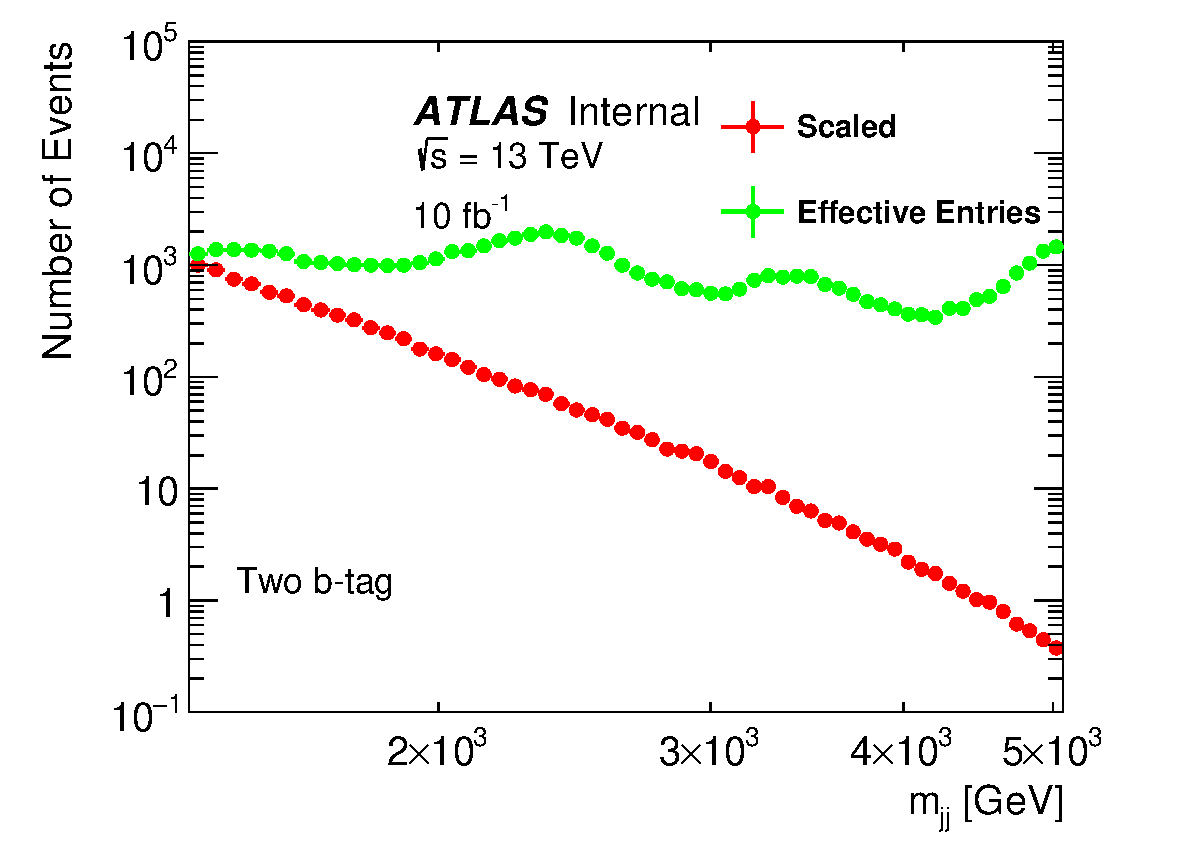
\includegraphics[width=0.5\linewidth, angle=0]{figs/Dibjet/ICHEP/FitRange/mbb_fix_8585_effEntries_Logx_10fb.pdf}}
   \hspace{-2mm}
   \subcaptionbox{$\geq$1 $b$-tag}{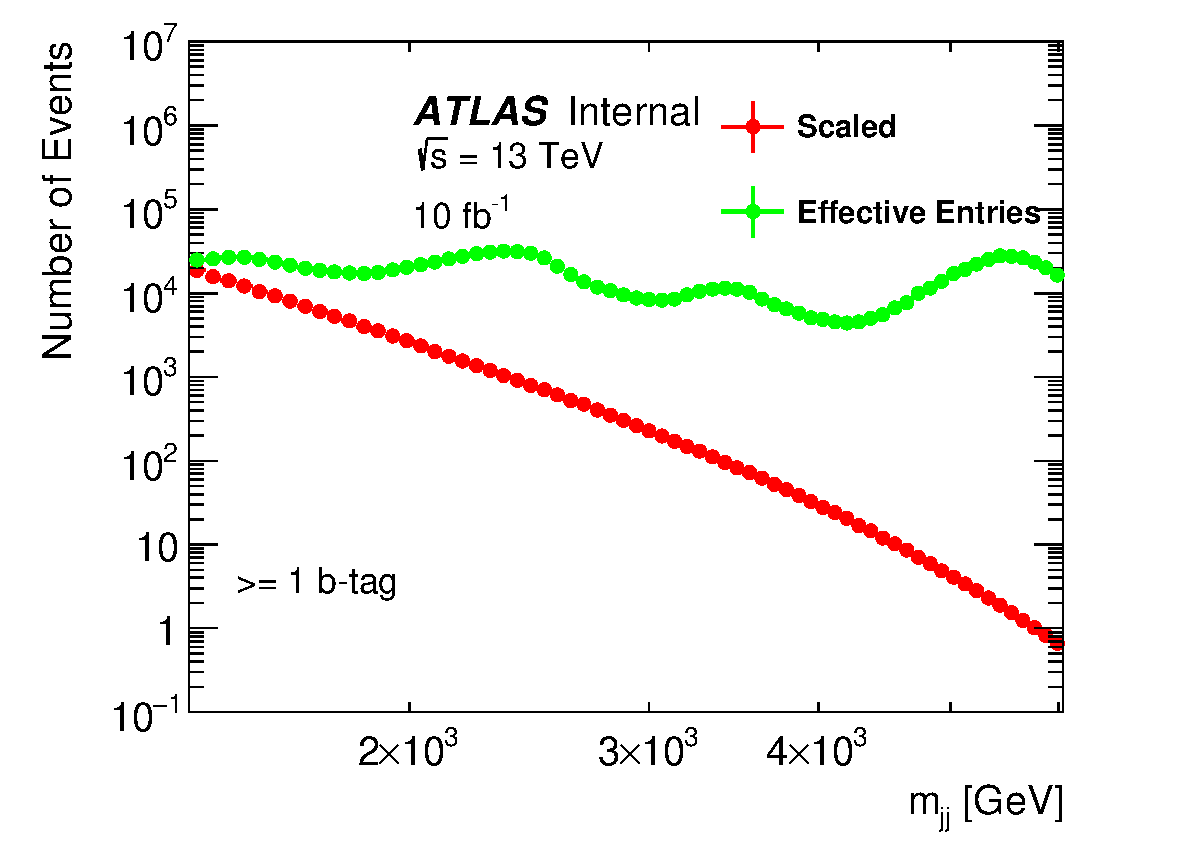
\includegraphics[width=0.5\linewidth, angle=0]{figs/Dibjet/ICHEP/FitRange/mbj_inc_fix_8585_effEntries_Logx_10fb.pdf}}
  \end{center}
  \vspace{-0.8em}
  \caption
      [The scaled and effective entries dijet mass spectra
        from QCD dijet simulation when the \summer{} data-set event selection has been applied.]
      {The scaled dijet mass spectrum (red) compared to the
        effective entries dijet mass spectrum (green)
        from QCD dijet simulation for the (a) 2 and (b) $\geq$1 $b$-tag category.
        The \summer{} data-set event selection has been applied.}
  \label{fig:effEnt}
\end{figure}

\subsection{Validation Studies: Dijet Mass Range Studies}
\label{sec:bkg-summer_range}

The first validation study performed is to show that the dijet fit functions are able to describe the dijet mass spectra in the mass range considered.
To perform this study the search phase is applied to the scaled dijet mass spectra from simulation, as described in the previous section.

For this validation study the dijet mass spectrum uses 
the statistical uncertainties of the simulated sample,
which are given by the square root of the number of effective entries.
10,000 pseudo-experiments are used to calculate \bh{} and \dhunt{} $p$-values, as will be done in all \summer{} search phase validation studies.
The initial dijet mass spectra are considered with the lower edge of the dijet mass spectrum at $m_{jj}$ = 1100 GeV,
selected such that there is no kinematic bias from the single jet trigger,
and an upper mass edge at the lowest dijet mass bin which contains less than one entry.

When performing the dijet mass range validation studies
the dijet fit function that would be used in the final data-set was not known.
Therefore, it was necessary to make a choice of the dijet fit function used to perform this study;
the 4 parameter dijet fit function was selected.
The 3 parameter dijet fit function was not chosen as it represents a special case
of the 4 parameter dijet fit function when one parameter ($p_4$) is set to zero.
The 5 parameter dijet fit function was not chosen as, at the time,
it had not been used or validated at previous dijet searches.

%Figure~\ref{fig:Short_4para_1100_figure1} and \ref{fig:Short_5para_1100_figure1} show the search phase
Figure~\ref{fig:Short_4para_1100_figure1} shows the search phase
for both $b$-tag categories, using the 4 parameter dijet fit function and the lower edge of the dijet mass spectrum at $m_{jj}$ = 1100 GeV.
The most discrepant excess is indicated by the blue lines and the \bh{} \mbox{$p$-value} of the excess is shown on the plot.
The lower panel shows the significance in each~dijet mass bin,
defined as the difference between the data and the background estimate divided by the statistical uncertainty of number of data events.
%Similarly, the \mbox{$p$-value} of the most discrepant deficit is calculated using the same process, which is referred to as \dhunt{},
%and an overall quality of fit \mbox{$p$-value} is also calculated by the same process using the $\chi^{2}$ test statistic.

%\vfill
%\newpage

In Figure~\ref{fig:Short_4para_1100_figure1} it is shown that, in the $\geq$1 $b$-tag category,
a discrepant excess is observed which has been assigned a \bh{} \mbox{$p$-value} of $<$0.0001
\footnote{This means that the observed \bh{} test-statistic was greater than in all 10,000 pseudo-experiments.}.
A \bh{} \mbox{$p$-value} of $<$0.0001 is also found when the search phase is performed using the 5 parameter dijet fit function.
This shows that the 4 and 5 parameter dijet fit functions provide a poor description
of the background dijet mass spectrum in the $\geq1$ $b$-tag category.
It can also be concluded that the 3 parameter dijet fit function will also be inadequate, as it is a subset of the 4 parameter dijet fit function.

\begin{figure}[!htb]
  \begin{center}
   \captionsetup[subfigure]{aboveskip=0pt,justification=centering}
   \subcaptionbox{2 $b$-tag}{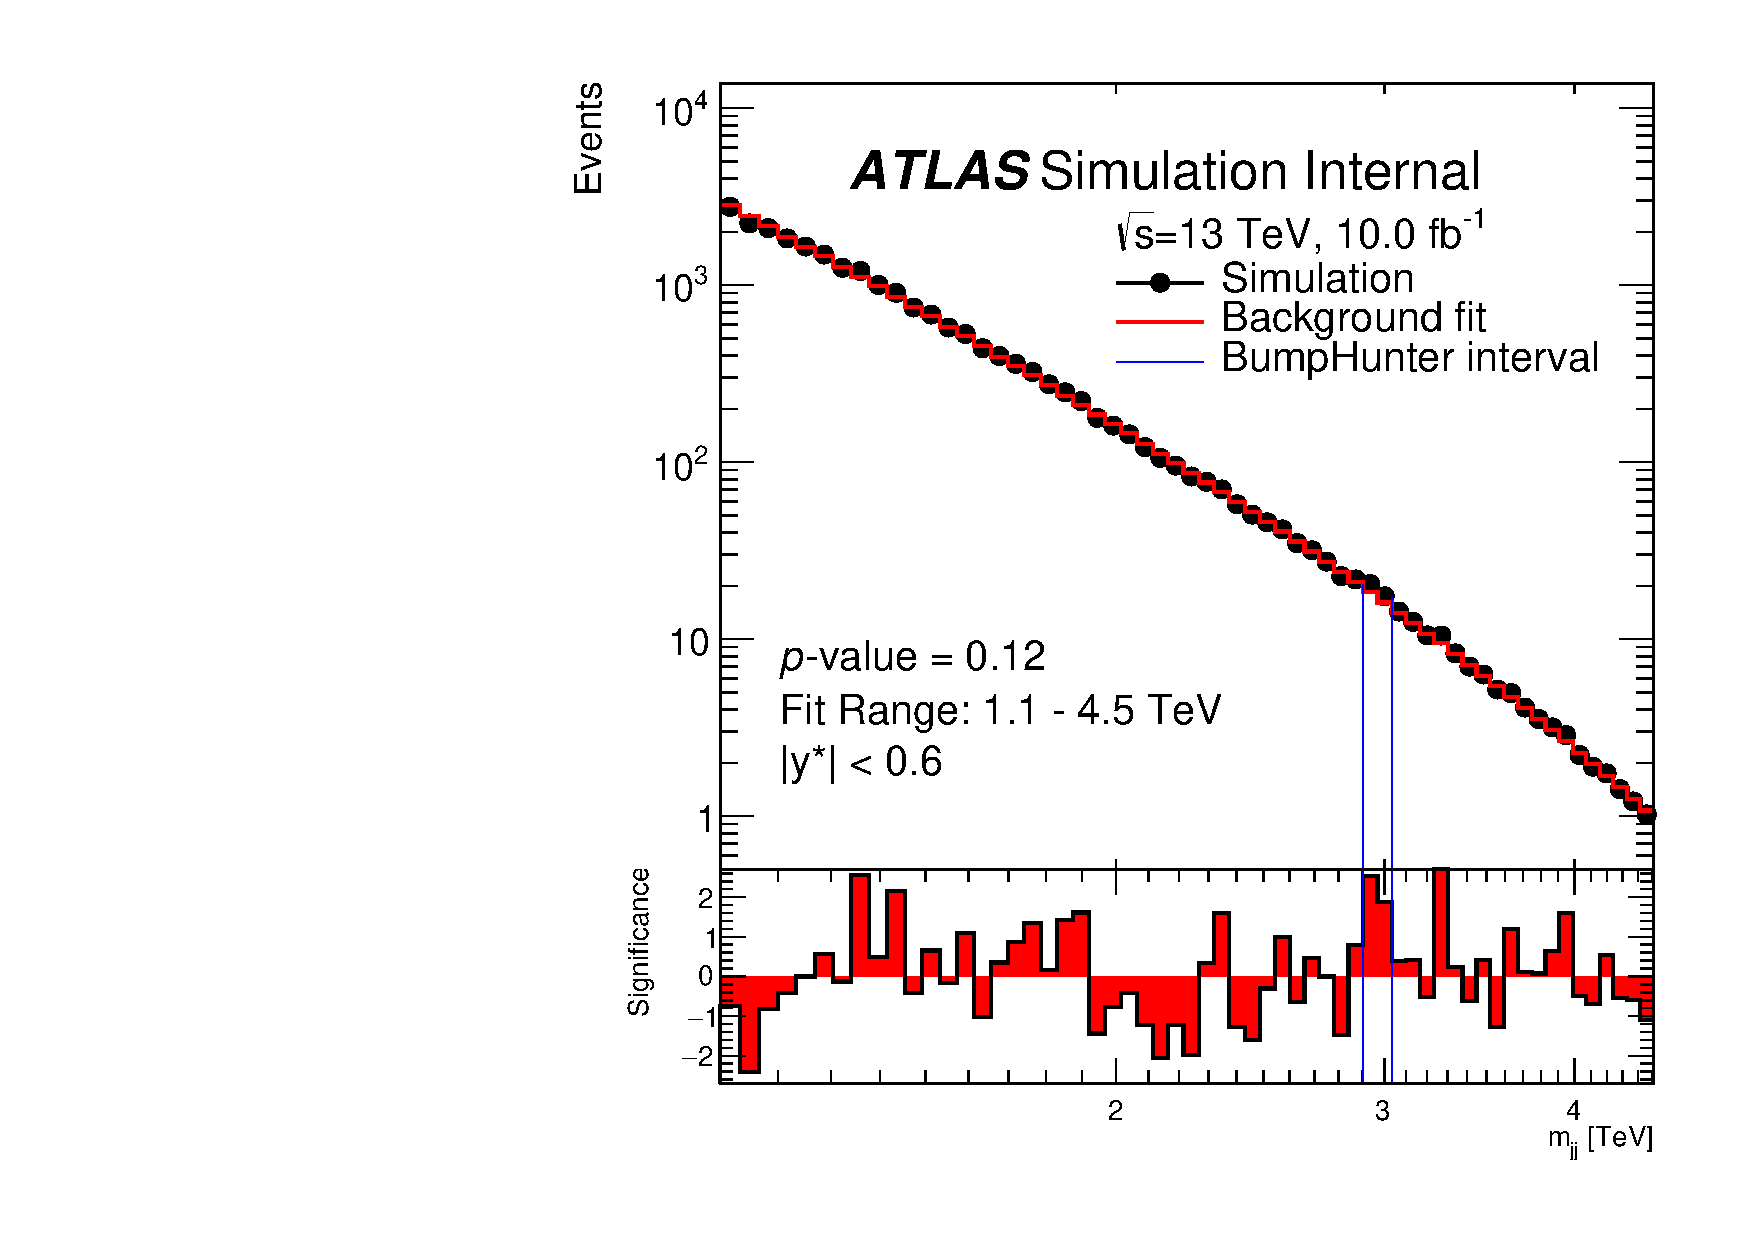
\includegraphics[width=0.4\linewidth, angle=0]{figs/Dibjet/ICHEP/FitRange/mbb_fix_8585_Short_4para_1100_figure1_10fb.pdf}}
   \subcaptionbox{$\geq$1 $b$-tag}{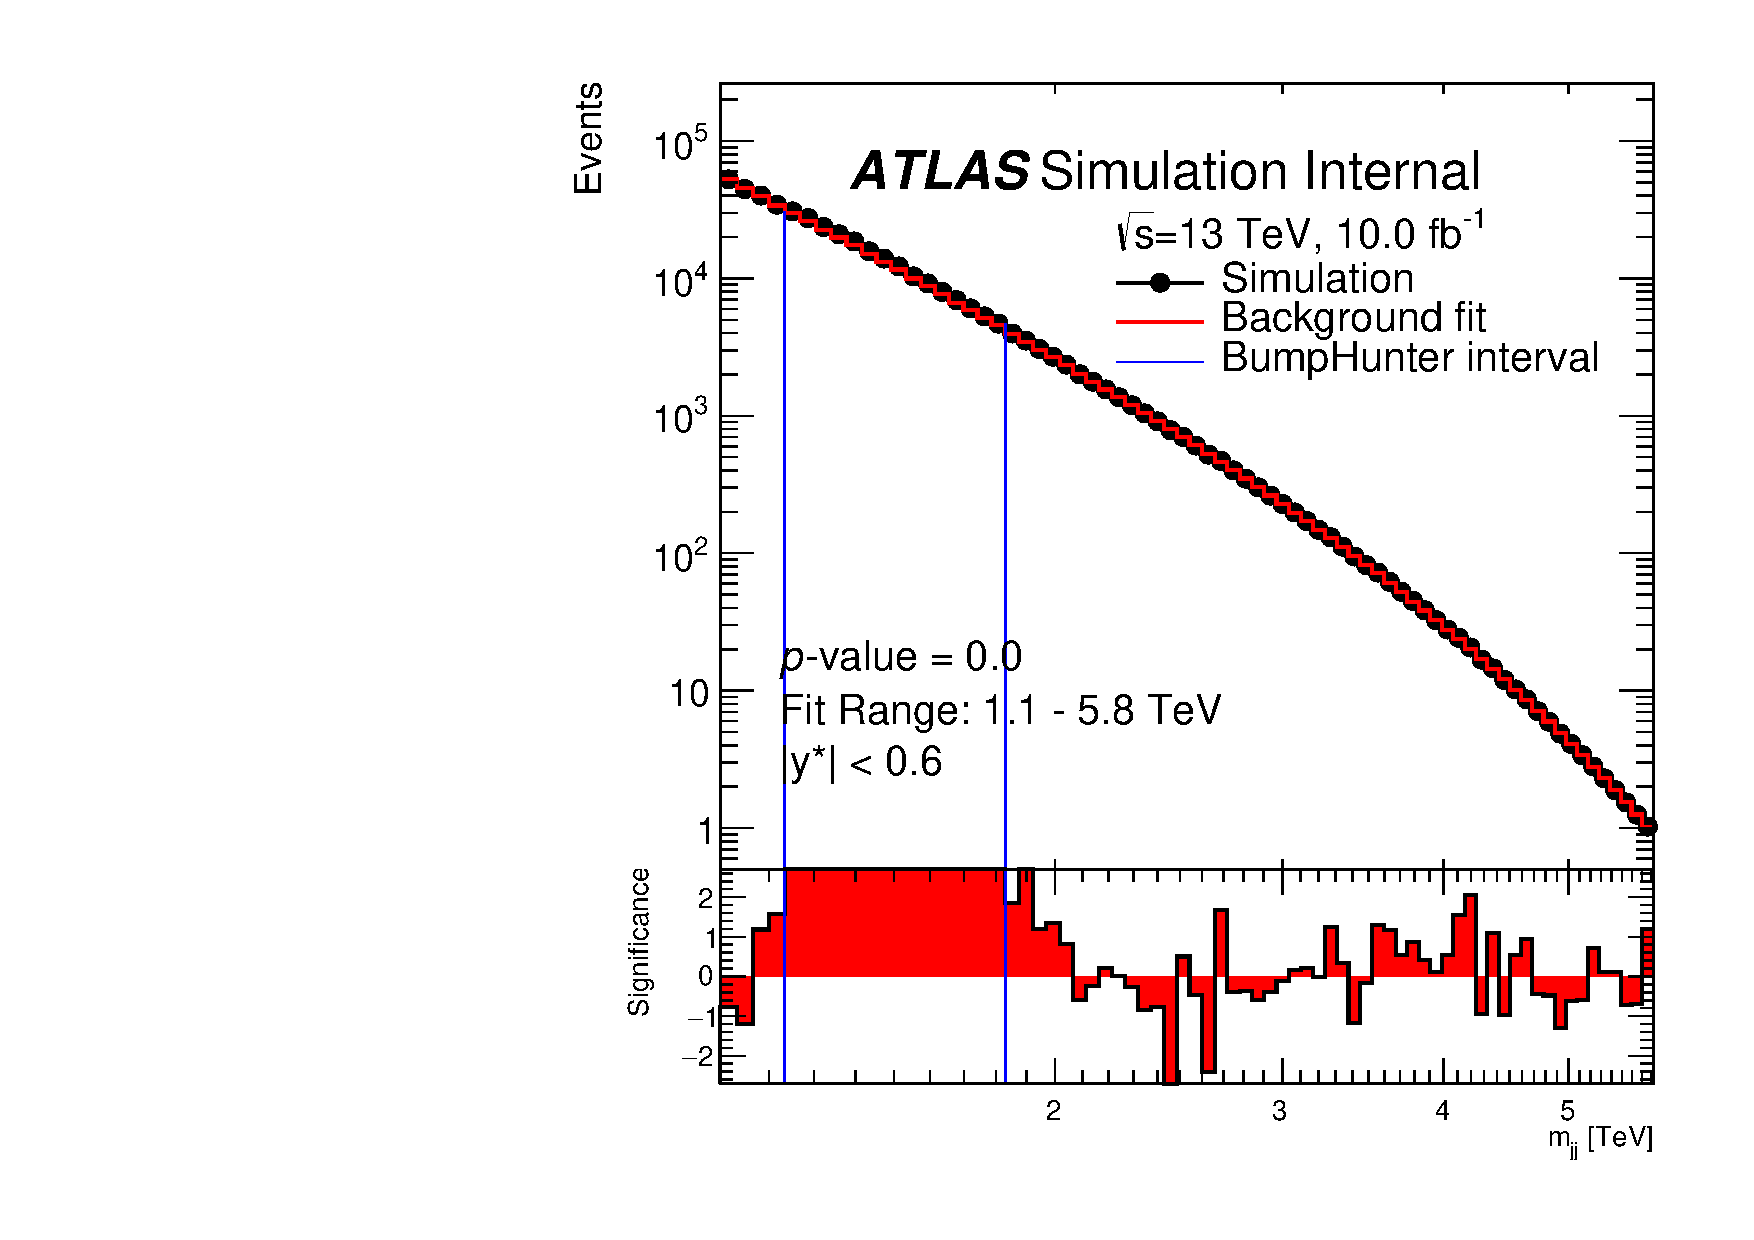
\includegraphics[width=0.4\linewidth, angle=0]{figs/Dibjet/ICHEP/FitRange/mbj_inc_fix_8585_Short_4para_1100_figure1_10fb.pdf}}
  \end{center}
  \vspace{-1em}
  \caption
      [The scaled dijet mass spectrum from QCD dijet simulation
        fitted to using the 4 parameter dijet fit function, with the lower edge of the dijet mass spectrum at 1100 GeV.
        The \summer{} data-set event selection has been applied.]
      {The scaled dijet mass spectrum from QCD dijet simulation for the (a) 2 and (b) $\geq$1 $b$-tag category,
        fitted to using the 4 parameter dijet fit function, with the lower edge of the dijet mass spectrum at 1100 GeV.
        The most discrepant excess as found by the \bh{} algorithm is indicated by the vertical blue lines and the \mbox{$p$-value} of this excess is printed on the plot.         
        The \summer{} data-set event selection has been applied.}
 \label{fig:Short_4para_1100_figure1}
\end{figure}
%
%
%\begin{figure}[!ht]
%  \begin{center}
%    \captionsetup[subfigure]{aboveskip=0pt,justification=centering}
%   \subcaptionbox{2 $b$-tag}{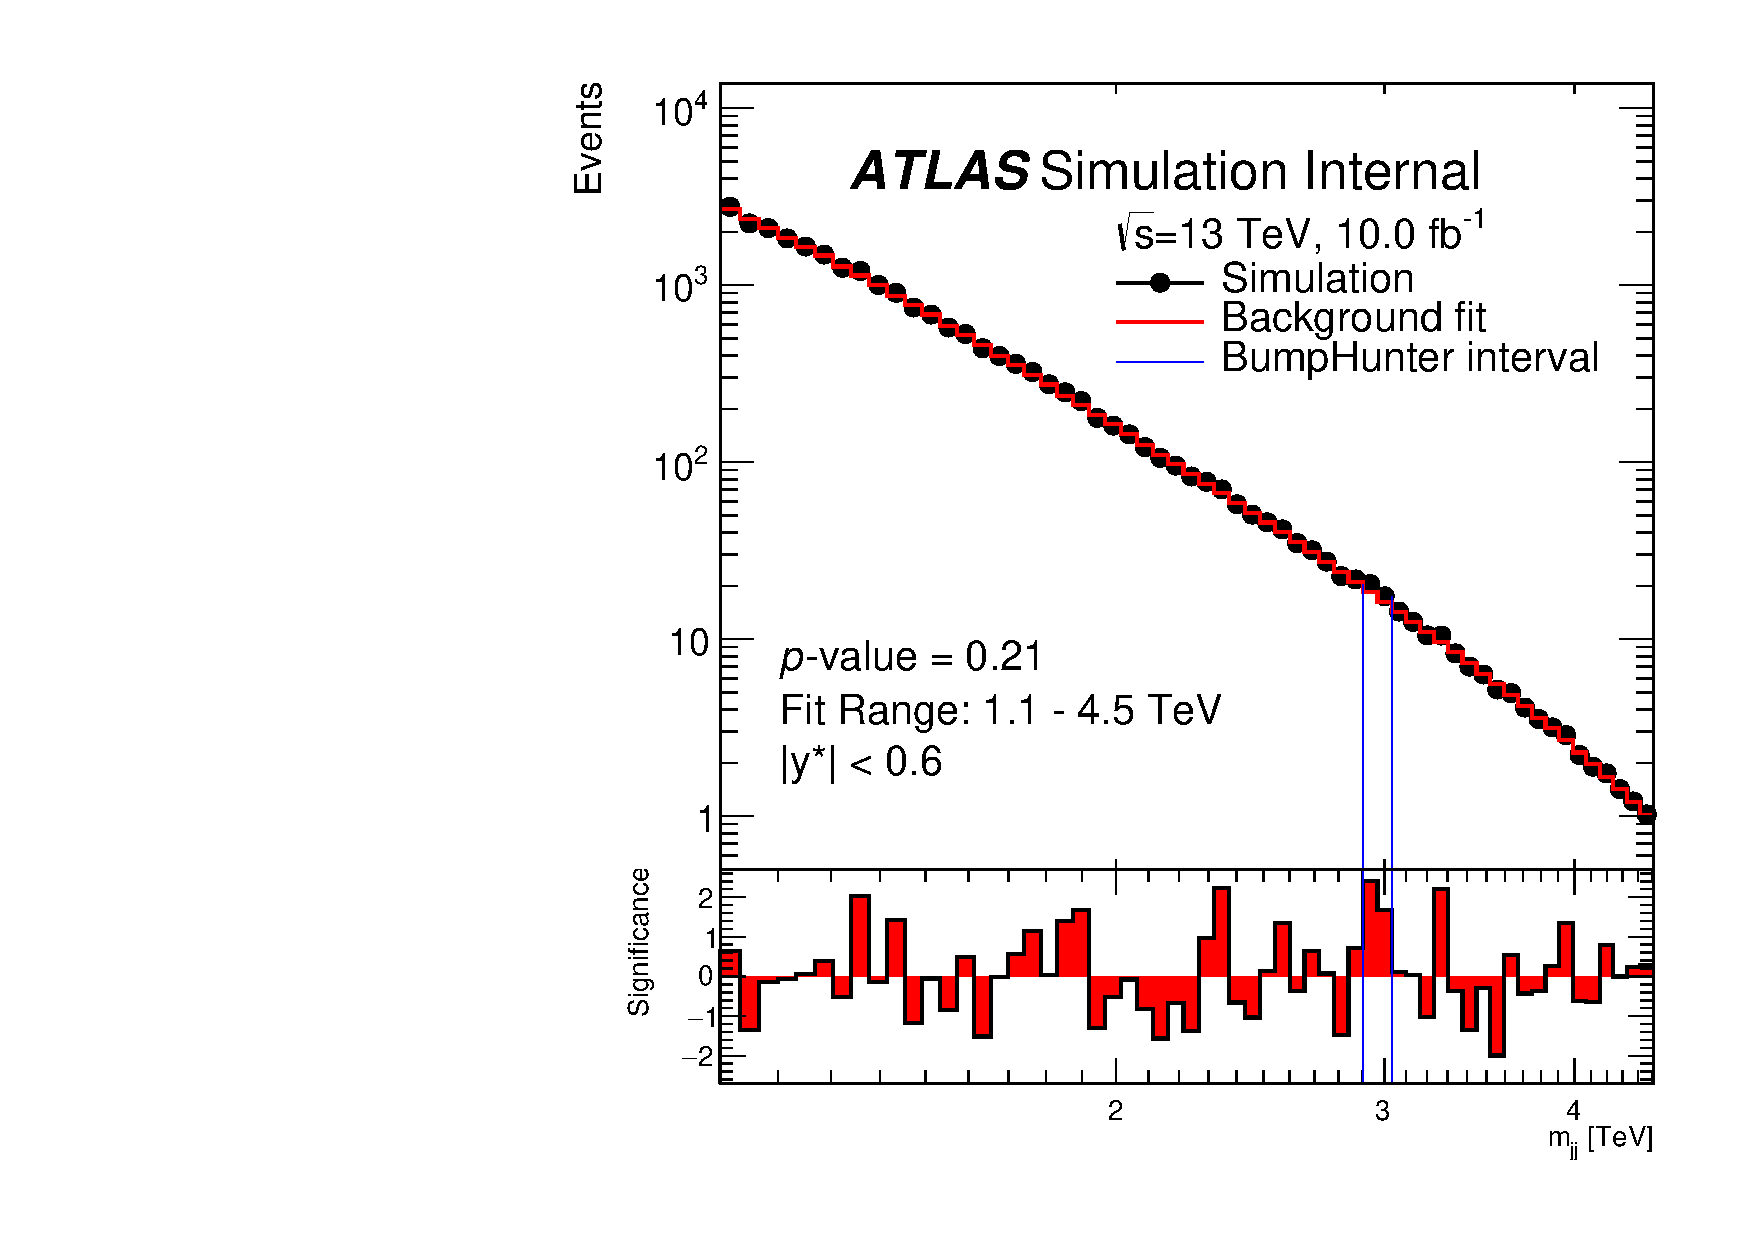
\includegraphics[width=0.4\linewidth, angle=0]{figs/Dibjet/ICHEP/FitRange/mbb_fix_8585_Short_5para_1100_figure1_10fb.pdf}}
%   \subcaptionbox{$\geq$1 $b$-tag}{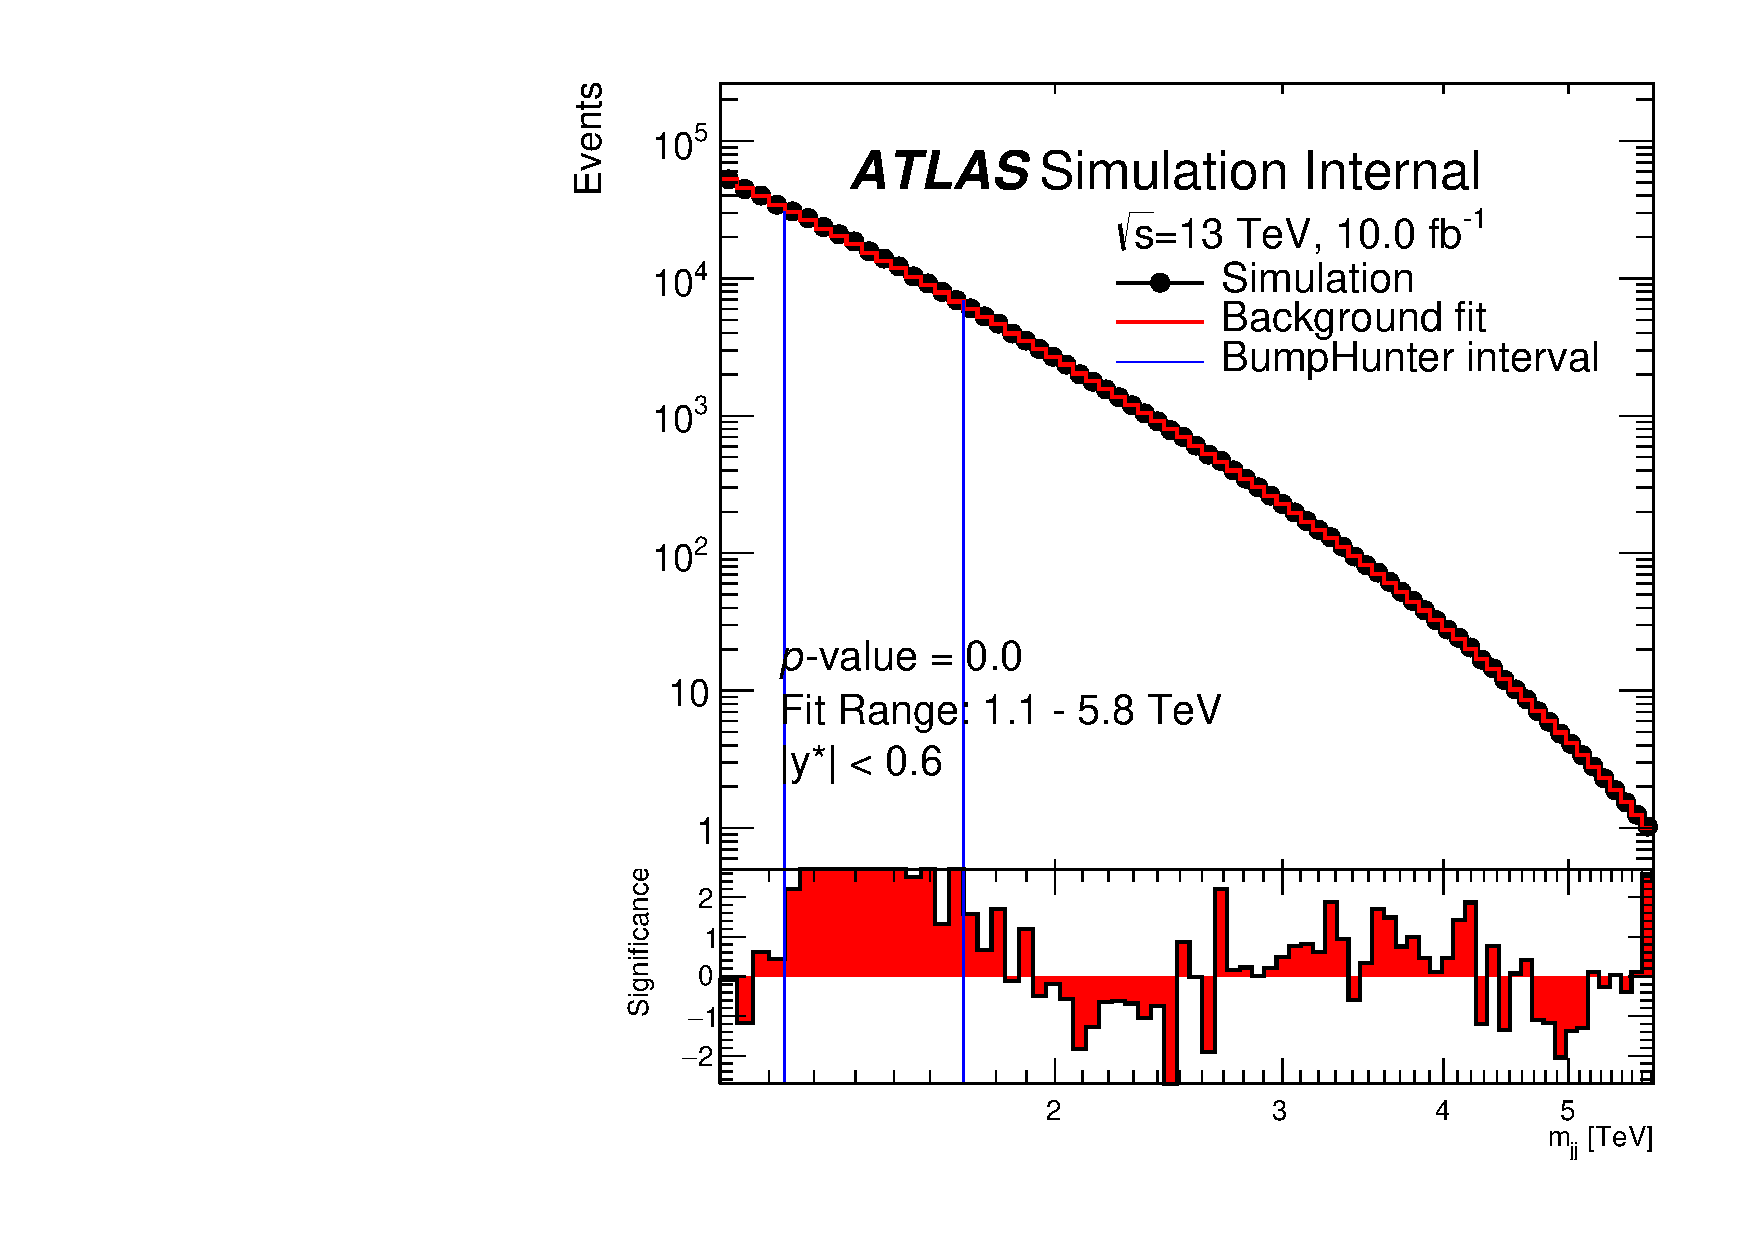
\includegraphics[width=0.4\linewidth, angle=0]{figs/Dibjet/ICHEP/FitRange/mbj_inc_fix_8585_Short_5para_1100_figure1_10fb.pdf}}
%  \end{center}
%  \caption{ The dijet mass spectrum from QCD dijet simulation for the (a) 2 and (b) $\geq$1 $b$-tag
%    category, fitted to using the 5 parameter dijet fit function, with the lower edge of the dijet mass spectrum at $m_{jj}$ = 1100 GeV.
%    The \bh{} algorithm is run to identify the most discrepant excess, as indicated by the blue lines.
%    Pseudo-experiments are used to assign the excess a \mbox{$p$-value}, which is shown on the plot.
%    The \summer{} data-set event selection has been applied.}
%  \label{fig:Short_5para_1100_figure1}
%\end{figure}

However, by changing the lower edge of the dijet mass spectrum,
a region can be found where the dijet fit functions are able to describe the background accurately.
To find the largest region with a stable fit quality, the simulated dijet mass spectrum is
fitted to using the 4 parameter dijet fit function with the lower edge of the dijet mass spectrum increased one bin at a time from 1100 to 1500 GeV.
%As before the upper edge of the dijet mass spectrum is the lowest mass bin that contains less than one entry.
For each lower edge considered
the \mbox{$p$-value} of the most discrepant excess is calculated using the \bh{} algorithm as before,
the \mbox{$p$-value} of the most discrepant deficit is calculated using the \dhunt{} algorithm,
and an overall quality of fit is represented using a $\chi^{2}$~\mbox{$p$-value}.
Figure~\ref{fig:mjjGraphs} shows the distributions of the
\bh{}, \dhunt{} and $\chi^{2}$ \mbox{$p$-value}s as the lower edge of the dijet mass spectra is increased
for both $b$-tag categories.
In both categories the background estimations are stable if the lower mass edge of the dijet mass spectrum is $m_{jj}$~=~1378 GeV or above.
This demonstrates that at low mass there are features in the background dijet mass spectrum that are causing a poor fit quality,
which can be removed by requiring that $m_{jj}~>$~1378 GeV. 

Figure~\ref{fig:Short_4para_1378_figure1} shows the search phase applied to the dijet mass spectra
of the simulated QCD dijet sample with a lower edge at $m_{jj}$~=~1378 GeV for both $b$-tag categories
 using the 4 parameter dijet fit function.
The most discrepant excess, as found by the \bh{} algorithm, is indicated by the blue lines
and the \mbox{$p$-value} of the excess is shown on the plot.
The study presented in this section motivates the requirement that $m_{jj}~>$~1378 GeV in the \summer{} data-set event selection.

\begin{figure}[!ht]
  \begin{center}
    \captionsetup[subfigure]{aboveskip=0pt,justification=centering}
   \subcaptionbox{2 $b$-tag}{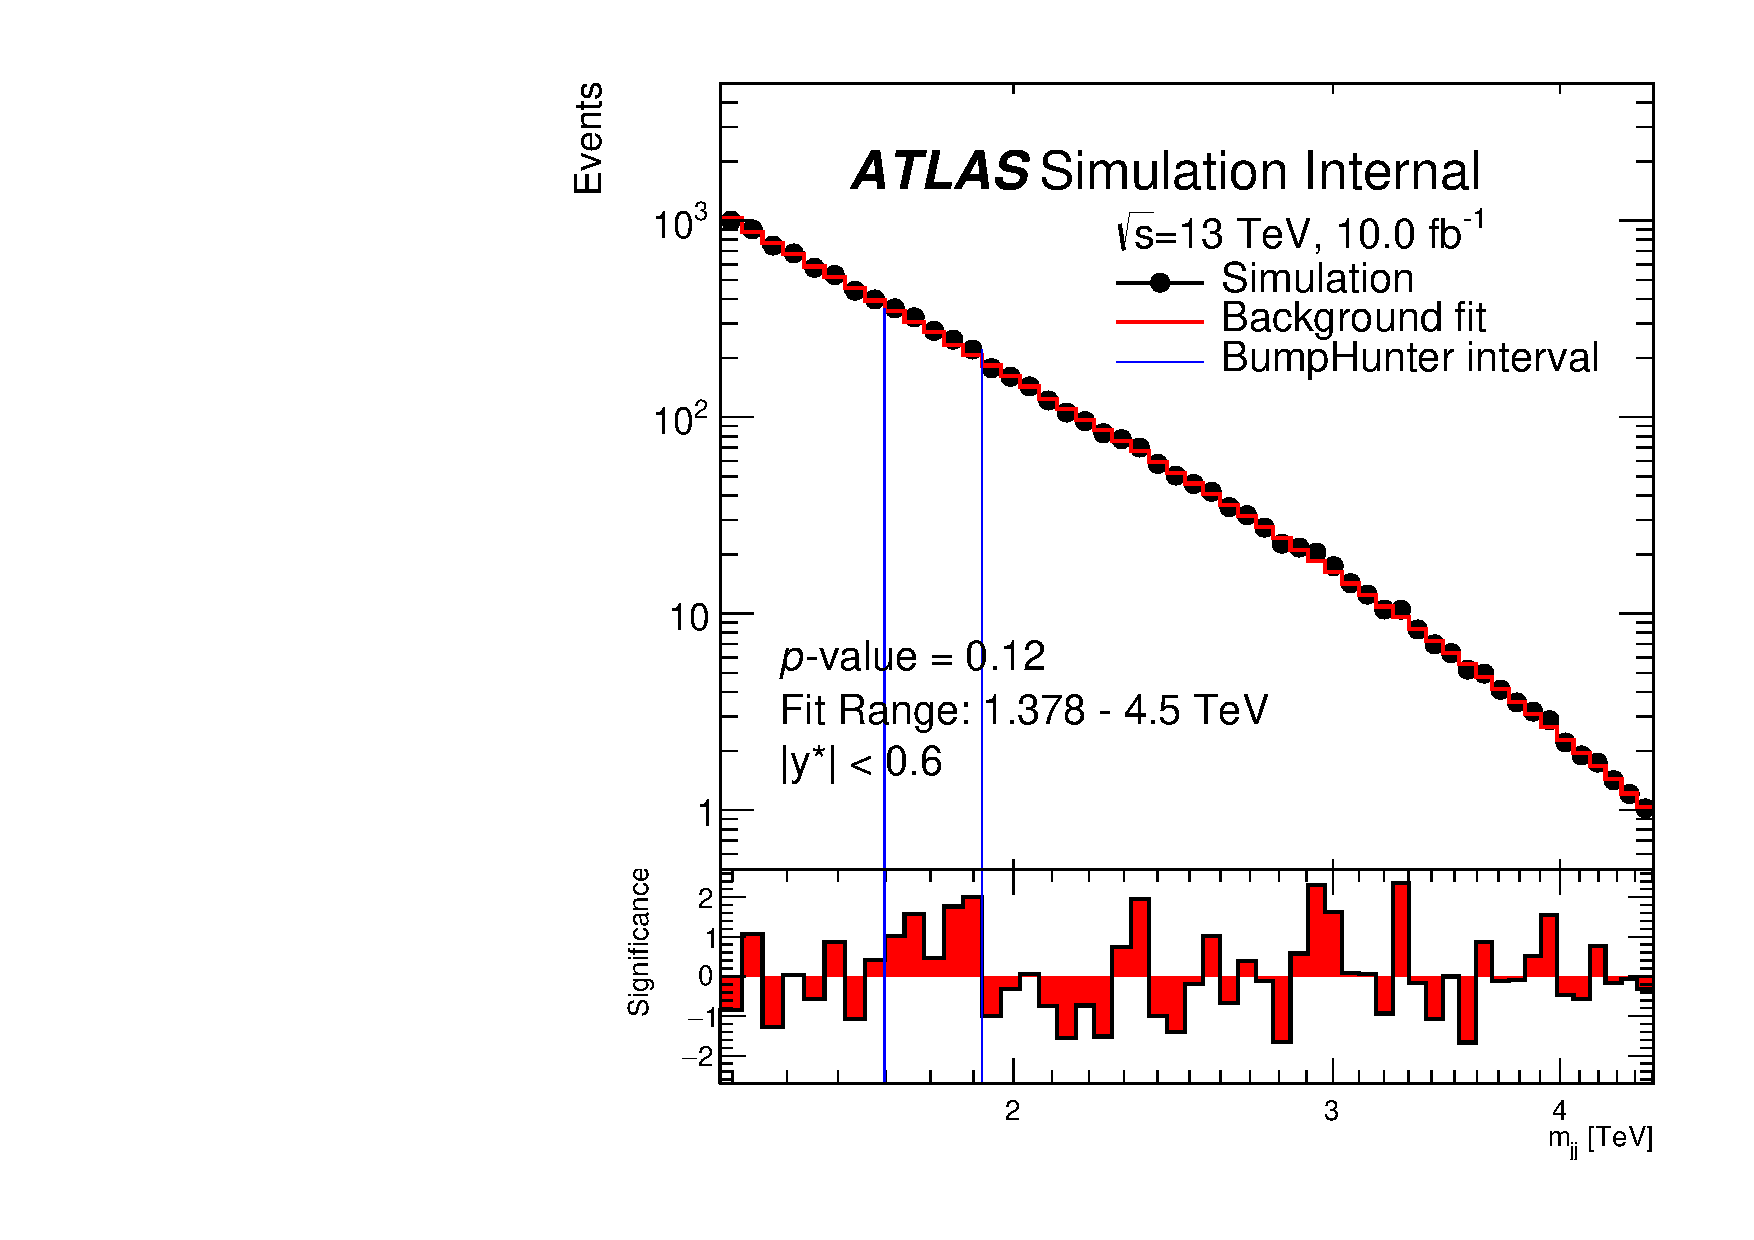
\includegraphics[width=0.4\linewidth, angle=0]{figs/Dibjet/ICHEP/FitRange/mbb_fix_8585_Short_4para_1378_figure1_10fb.pdf}}
   \subcaptionbox{$\geq$1 $b$-tag}{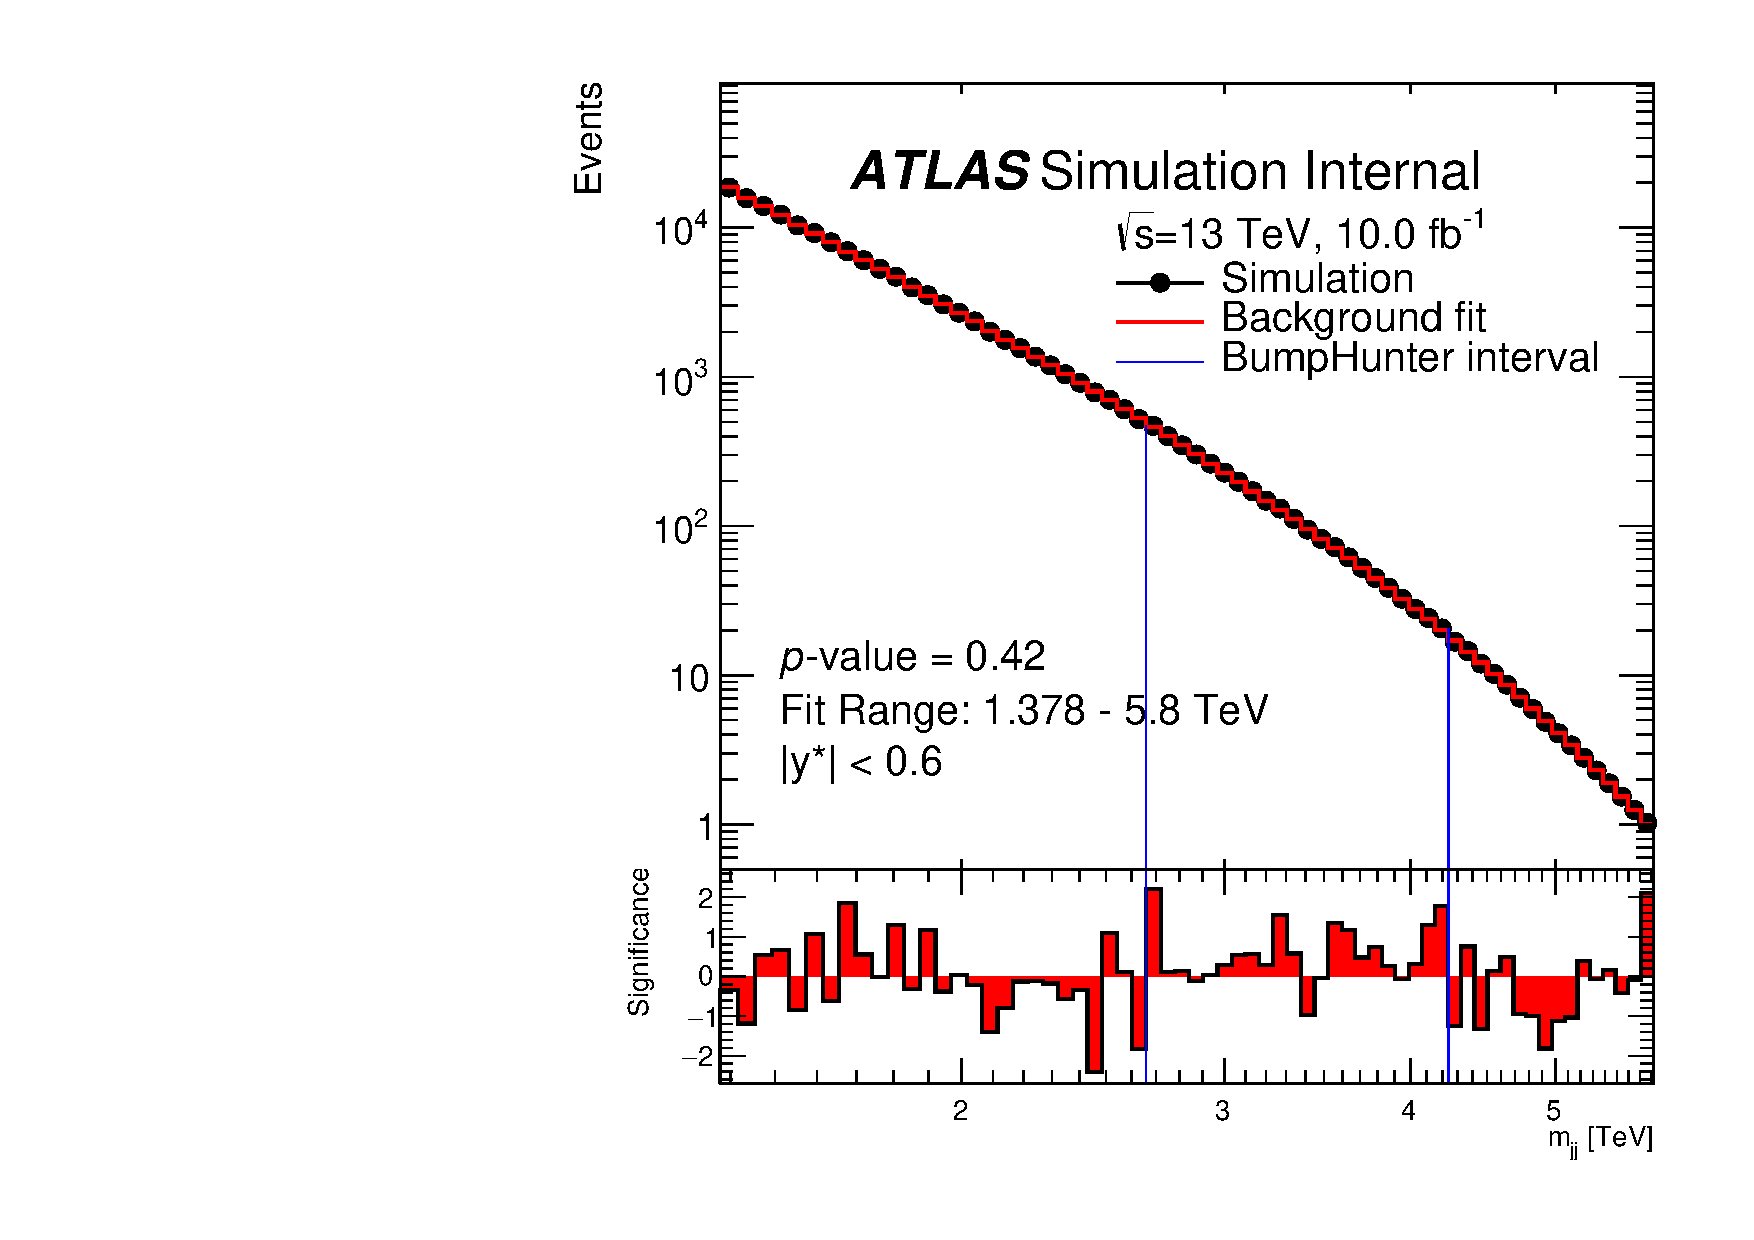
\includegraphics[width=0.4\linewidth, angle=0]{figs/Dibjet/ICHEP/FitRange/mbj_inc_fix_8585_Short_4para_1378_figure1_10fb.pdf}}
  \end{center}
  \vspace{-1em}
  \caption
      [The scaled dijet mass spectrum from QCD dijet simulation
        fitted to using the 4 parameter dijet fit function, with the lower edge of the dijet mass spectrum at 1378 GeV.
        The \summer{} data-set event selection has been applied.]
      { The scaled dijet mass spectrum from QCD dijet simulation for the (a) 2 and (b) $\geq$1 $b$-tag  category,
       fitted to using the 4 parameter dijet fit function, with the lower edge of the dijet mass spectrum at 1378 GeV.
       The most discrepant excess as found by the \bh{} algorithm is indicated by the vertical blue lines and the \mbox{$p$-value} of this excess is printed on the plot.
       The \summer{} data-set event selection has been applied.}
  \label{fig:Short_4para_1378_figure1}
\end{figure}

\begin{figure}[!htb]
  \begin{center}
    \captionsetup[subfigure]{aboveskip=0pt,justification=centering}
    \subcaptionbox{\bh{} $p$-value,\\2 $b$-tag}{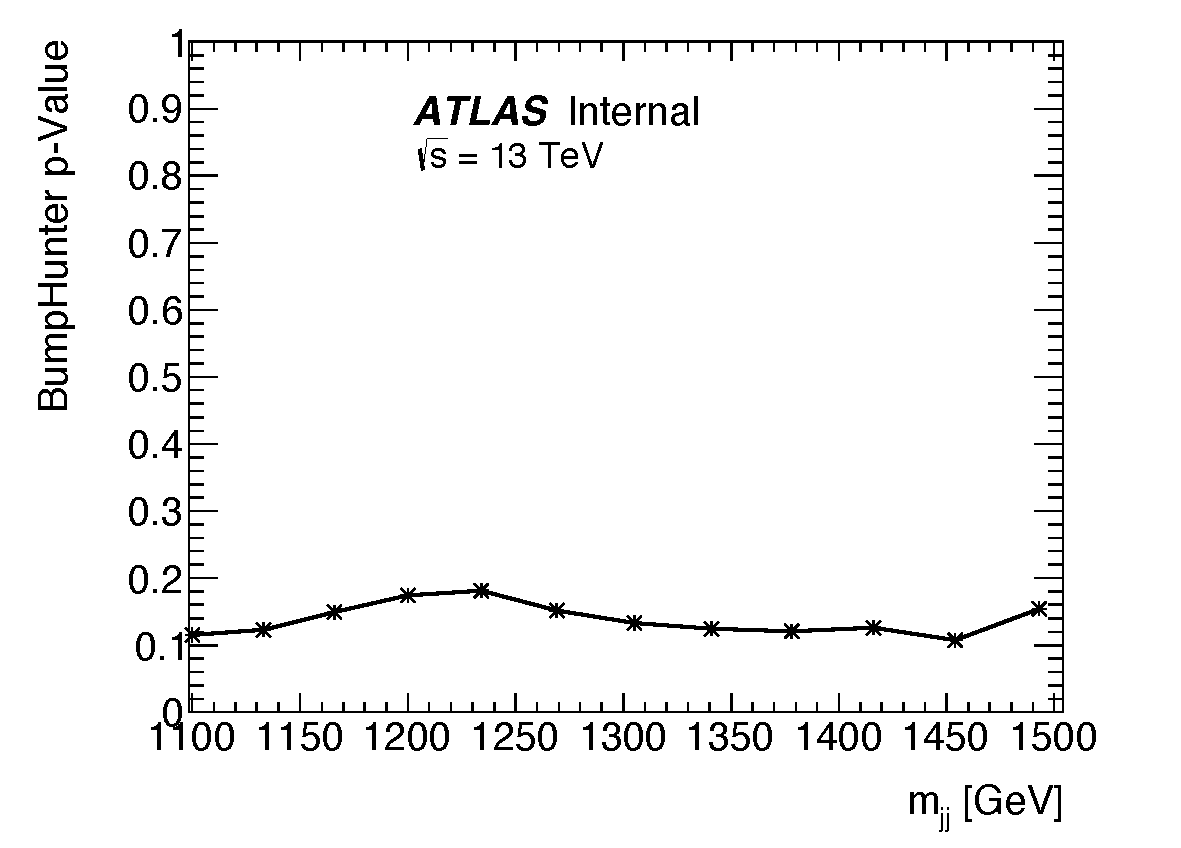
\includegraphics[width=0.45\linewidth, angle=0]{figs/Dibjet/ICHEP/FitRange/mbb_fix_8585_mjjGraph_bumpHunter_10fb.pdf}}
    \subcaptionbox{\bh{} $p$-value,\\$\geq1~b$-tag}{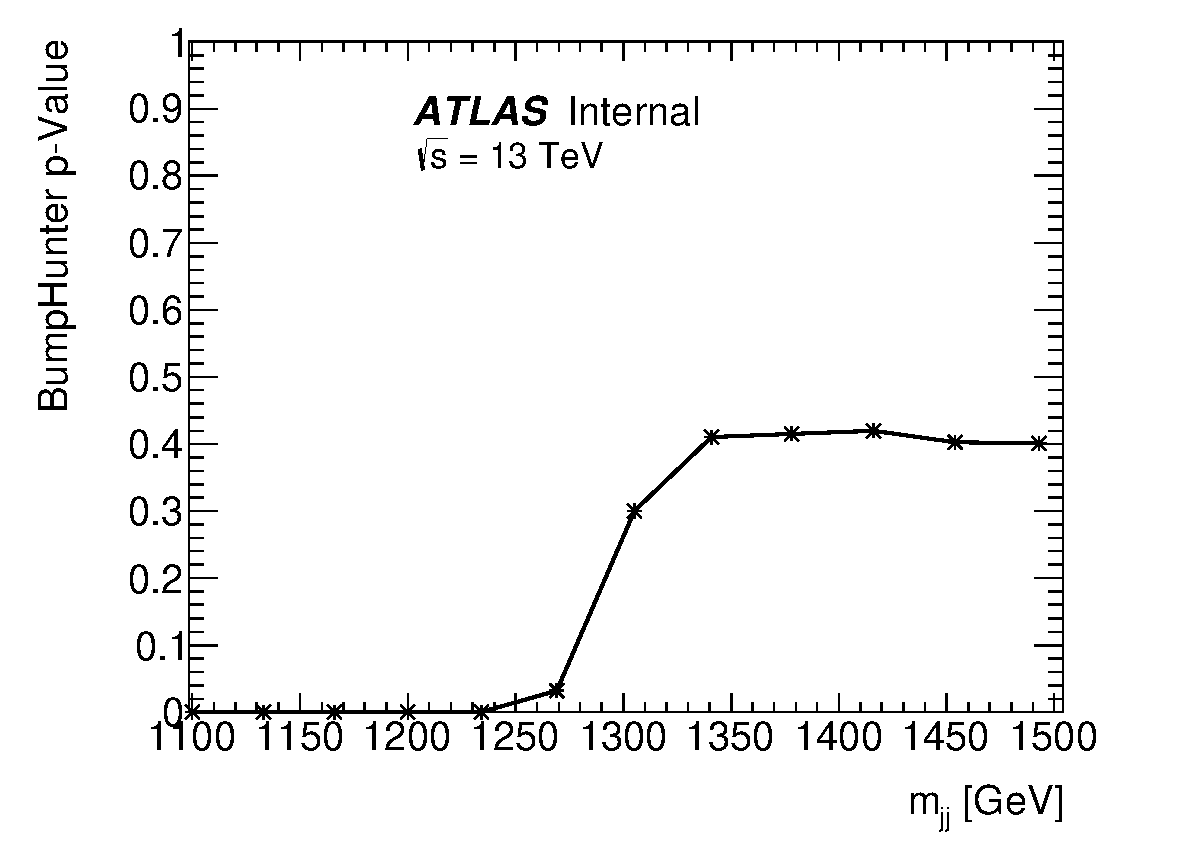
\includegraphics[width=0.48\linewidth, angle=0]{figs/Dibjet/ICHEP/FitRange/mbj_inc_fix_8585_mjjGraph_bumpHunter_10fb.pdf}}\\\vspace{0.3em}
    \subcaptionbox{\dhunt{} $p$-value,\\2 $b$-tag}{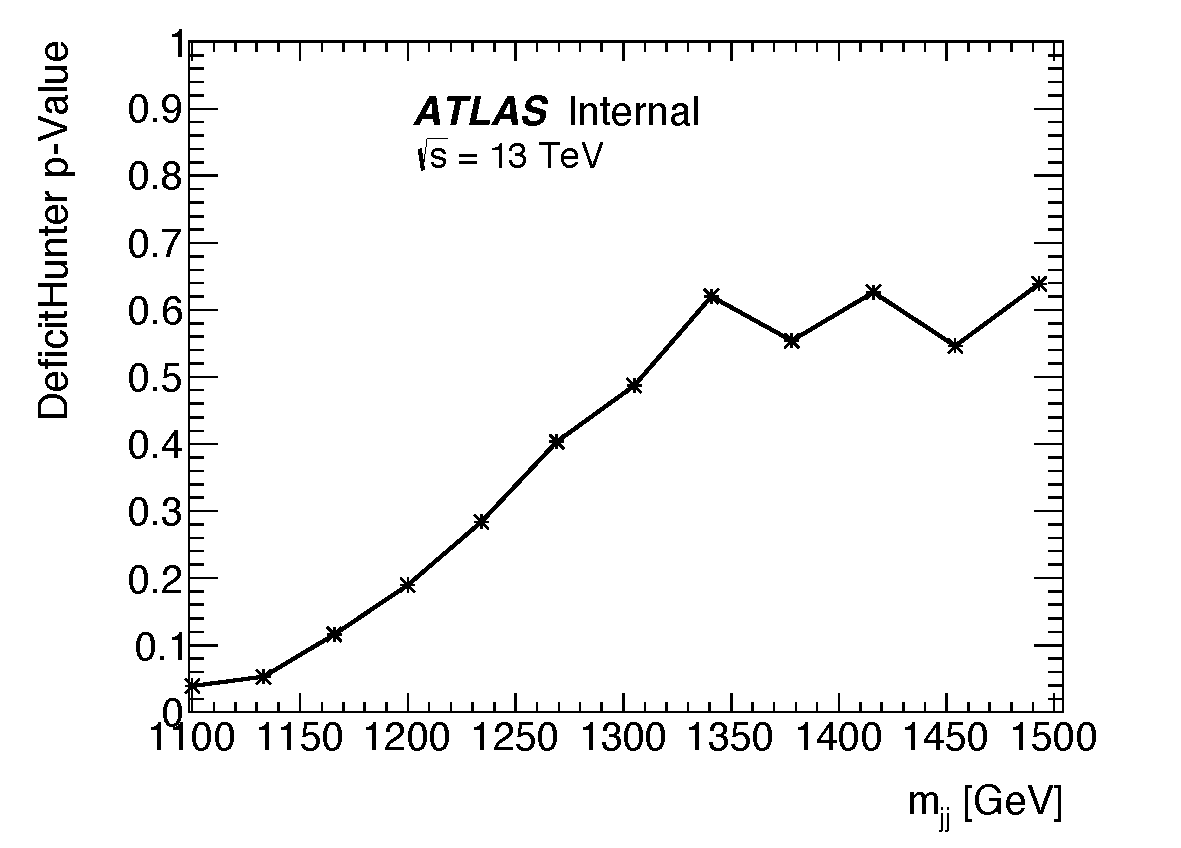
\includegraphics[width=0.45\linewidth, angle=0]{figs/Dibjet/ICHEP/FitRange/mbb_fix_8585_mjjGraph_deficitOnlyHunter_10fb.pdf}}
    \subcaptionbox{\dhunt{} $p$-value,\\$\geq1~b$-tag}{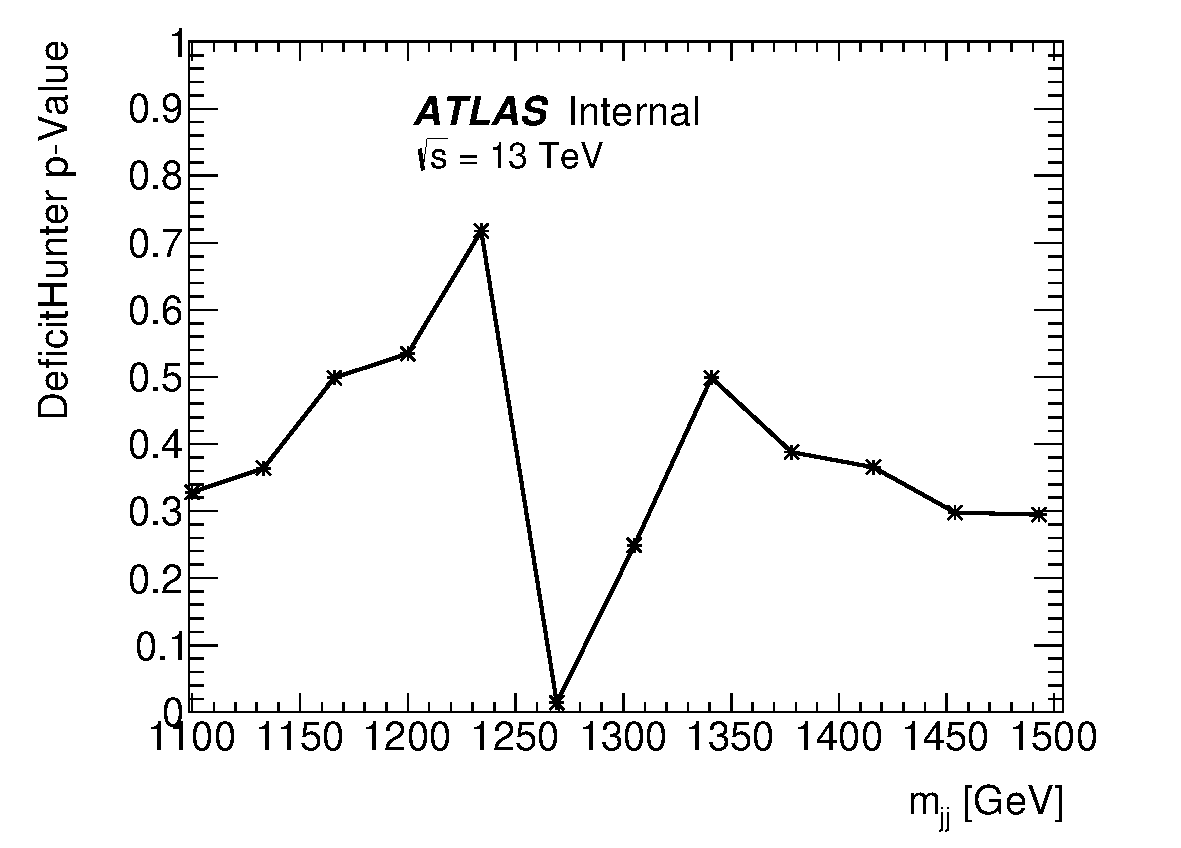
\includegraphics[width=0.48\linewidth, angle=0]{figs/Dibjet/ICHEP/FitRange/mbj_inc_fix_8585_mjjGraph_deficitOnlyHunter_10fb.pdf}}\\\vspace{0.3em}
    \subcaptionbox{$\chi^{2}$ $p$-value,\\2 $b$-tag}{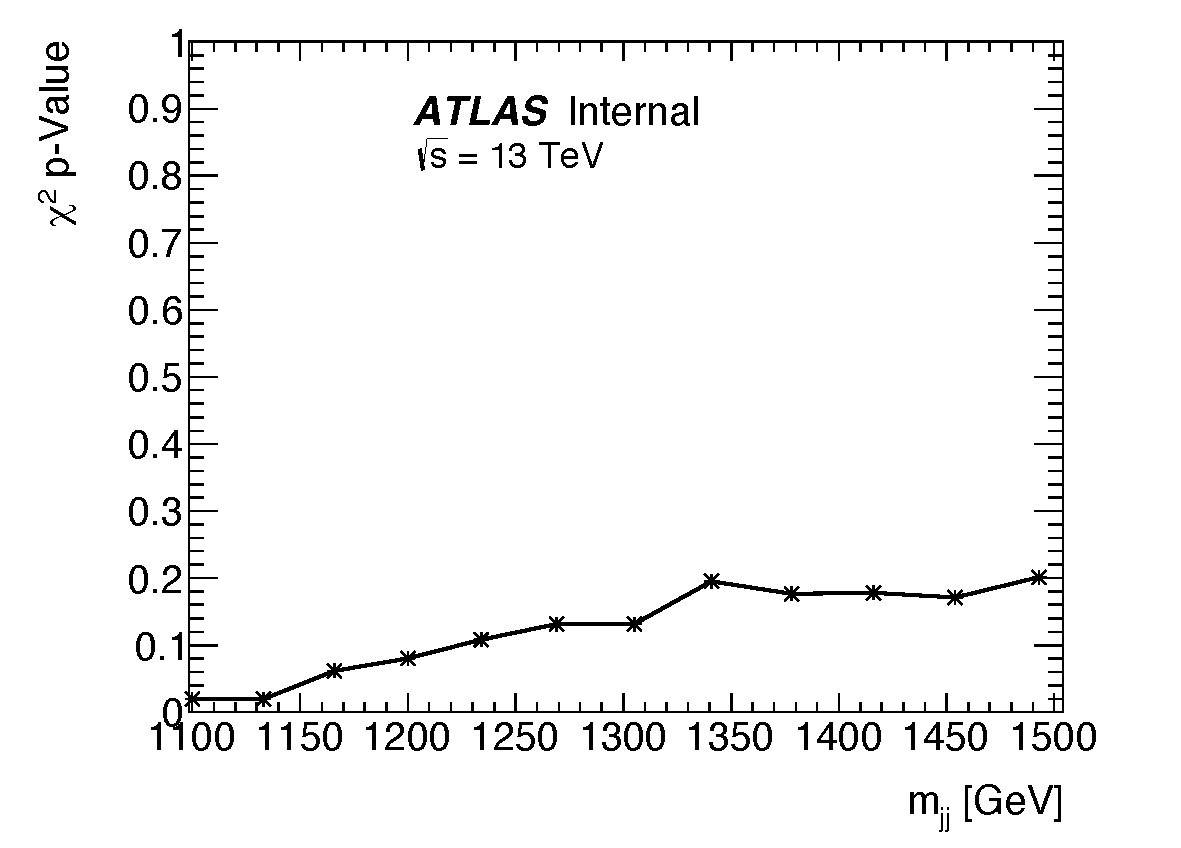
\includegraphics[width=0.45\linewidth, angle=0]{figs/Dibjet/ICHEP/FitRange/mbb_fix_8585_mjjGraph_chi2_10fb.pdf}}
    \subcaptionbox{$\chi^{2}$ $p$-value,\\$\geq1~b$-tag}{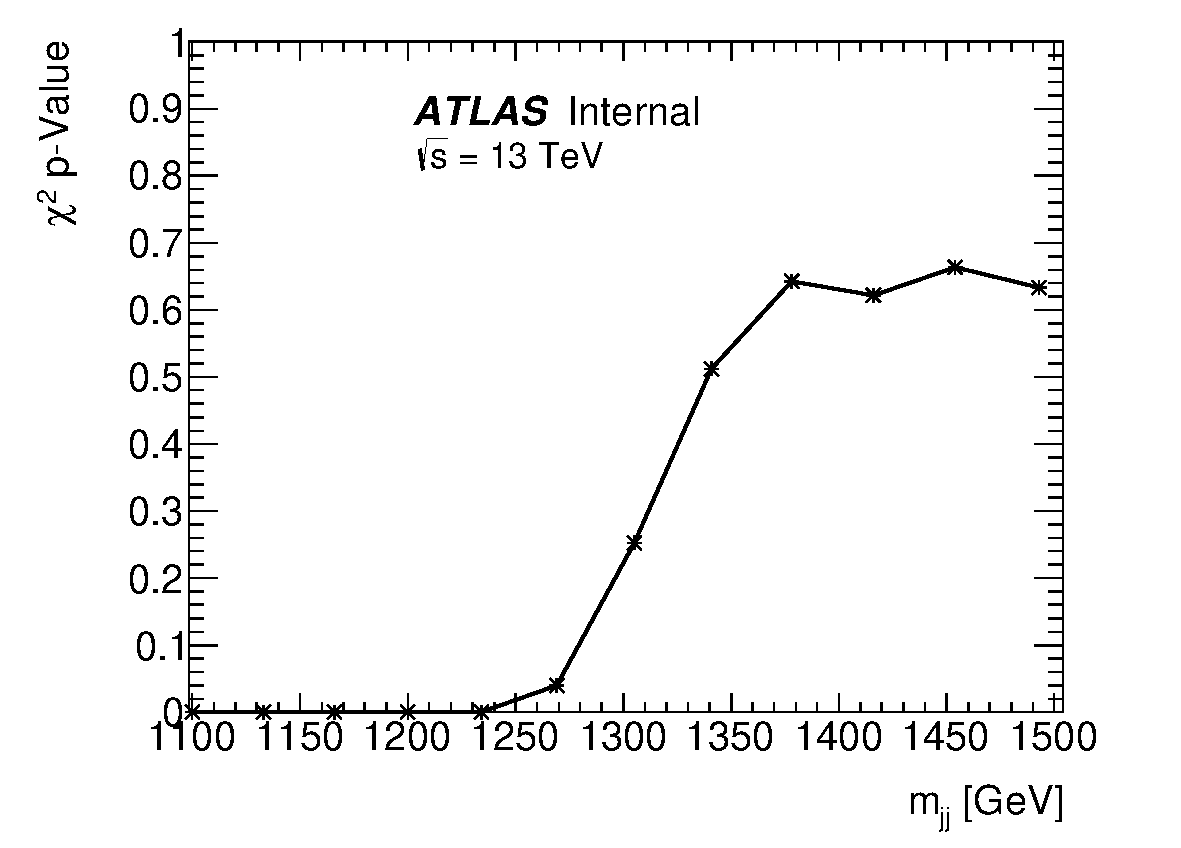
\includegraphics[width=0.48\linewidth, angle=0]{figs/Dibjet/ICHEP/FitRange/mbj_inc_fix_8585_mjjGraph_chi2_10fb.pdf}}
  \end{center}
  \vspace{-1em}
  \caption
      [The \bh{},  \dhunt{}  and $\chi^{2}$ \mbox{$p$-value}s
      for search phases performed to the scaled dijet mass spectrum from QCD dijet simulation
      as a function of the lower edge of the dijet mass spectrum.
      The \summer{} data-set event selection has been applied.]
      {The \bh{} (top row),  \dhunt{} (middle row) and $\chi^{2}$ (bottom row) \mbox{$p$-value}s
       for search phases performed to the scaled dijet mass spectrum from QCD dijet simulation
       using the 4 parameter dijet fit function
       for the 2 $b$-tag category (left column) and $\geq1~b$-tag category (right column)
       as a function of the lower edge of the dijet mass ($m_{jj}$) spectrum.
       The \summer{} data-set event selection has been applied.}
  \label{fig:mjjGraphs}
\end{figure}


\FloatBarrier
\vfill
\clearpage
\subsection{Fit Function Selection}
\label{sec:bkg-summer_wilks}

With the range of the dijet mass spectrum selected using Monte-Carlo, shown in the previous section,
the dijet fit function is then selected using the final dijet mass spectrum from data and the Wilks' $p$-value described in Section~\ref{sec:bkg-wilks}.
The exact function selection procedure is as follows:
using the dijet mass spectrum the Wilks' \mbox{$p$-value} is calculated with
the 3 parameter dijet function as the nominal function and the 4 parameter dijet fit function as the alternate function.
If the Wilks' \mbox{$p$-value} is less than 0.05, the nominal fit function is rejected and the alternate function becomes the nominal.
The process is iteratively run until a dijet fit function with a Wilks' \mbox{$p$-value} \gt{} 0.05 is selected.

For the \summer{} data-set the choice of the dijet fit function was fixed using a 8.8~\ifb{} subset of data.
A subset was used such that the function choice could be finalised before the full data-set was collected;
this meant that the analysis strategy and search phase validation studies could be scrutinised by other members of the ATLAS collaboration before the conference note publication.
With hindsight, I think it would have been more rigorous to calculate Wilks' \mbox{$p$-value} on the full data-set.

Figure~\ref{fig:bkg-summer-wilks} shows the Wilks' \mbox{$p$-value} as a function of luminosity
for the $\geq1$ and 2 \mbox{$b$-tag} categories for the 8.8~\ifb{} subset of data.
For both categories the 3 parameter dijet fit function when compared to the 4 parameter dijet fit function
has a Wilks' \mbox{$p$-value} $>$ 0.05,
therefore the 3 parameter dijet fit function is selected in both categories.
Given that the 3 parameter dijet fit function adequately describes the dijet mass spectra of the
majority of the data-set it is concluded that it has sufficient parameters to describe the dijet mass spectrum of the full data-set.

\begin{figure}[!htb]
  \begin{center}
    \captionsetup[subfigure]{aboveskip=0pt,justification=centering}
   \subcaptionbox{2 $b$-tag}{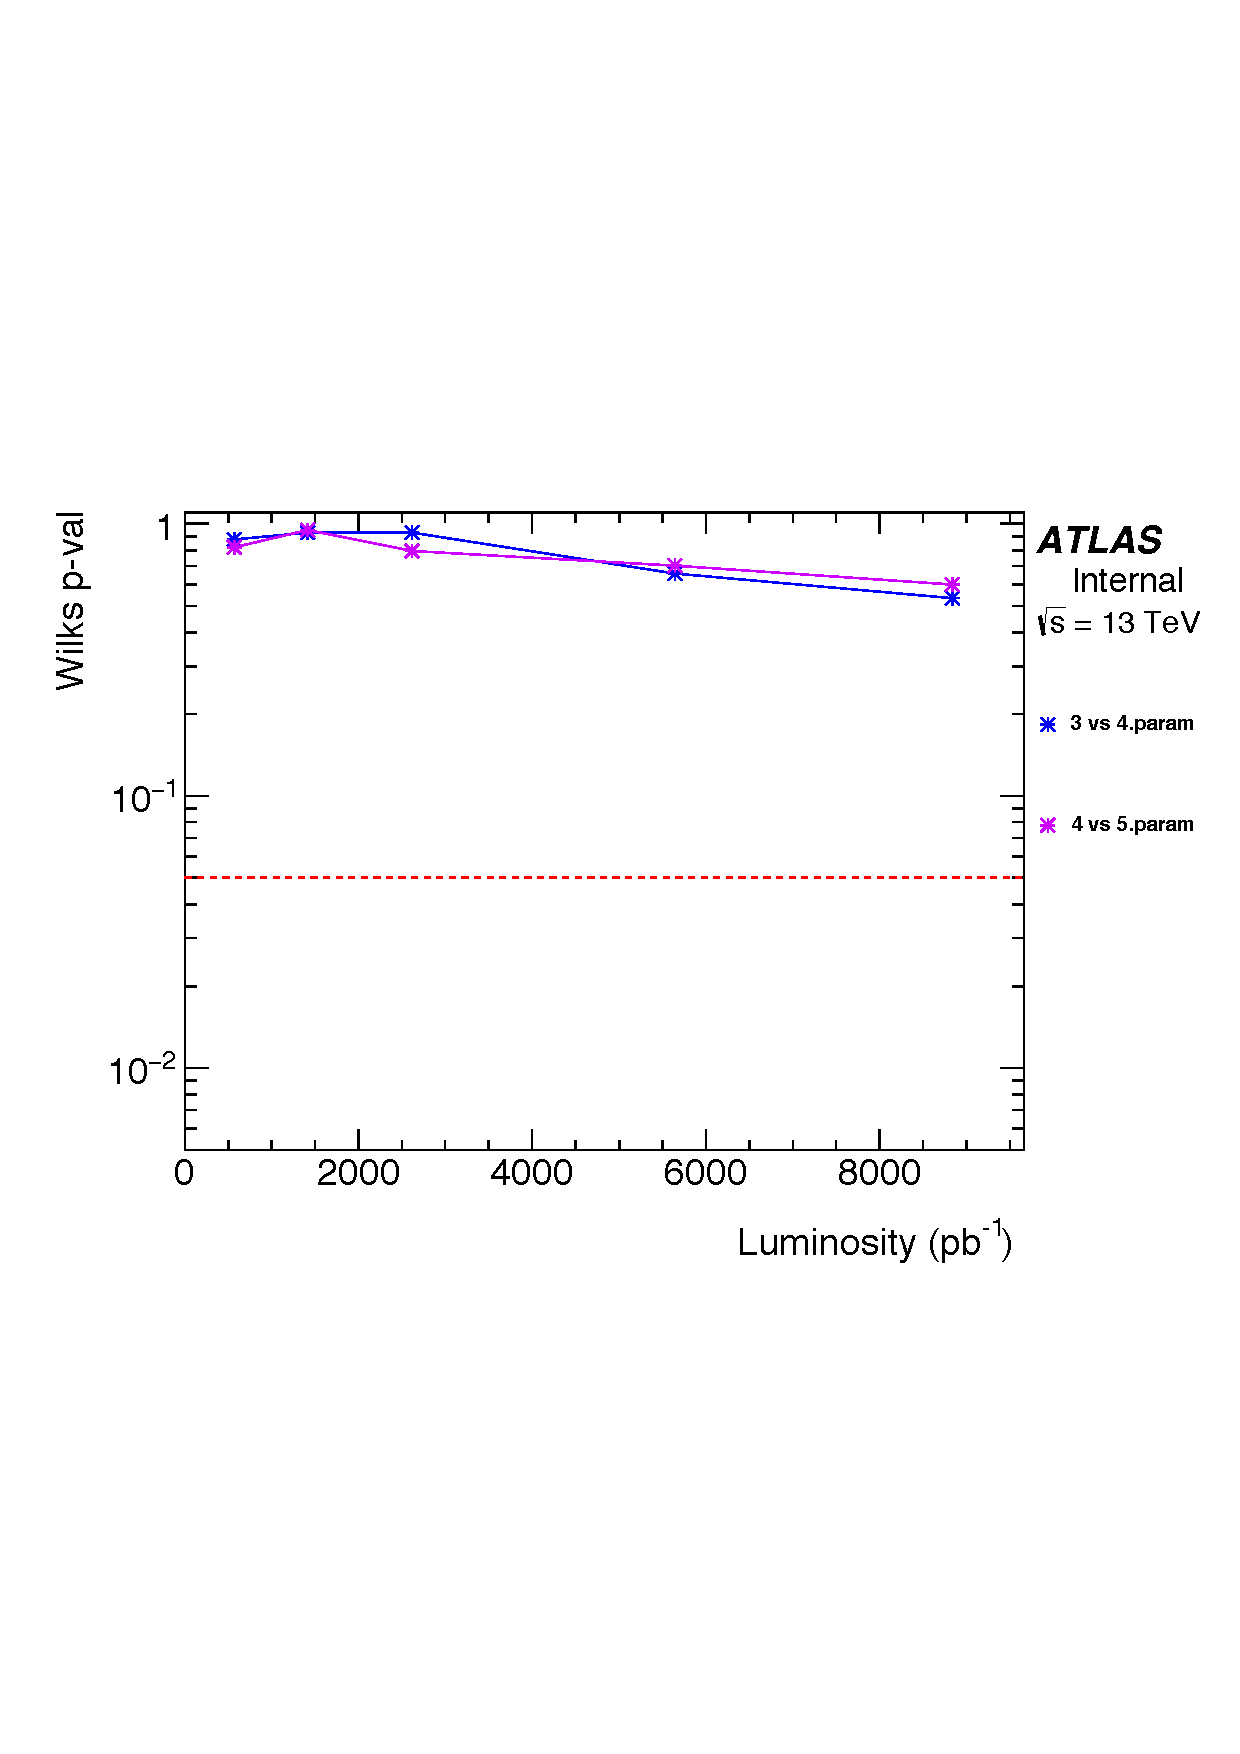
\includegraphics[width=0.8\linewidth, angle=0]{figs/Dibjet/ICHEP/bkg-WilksStat_bb.pdf}}\vspace{2em}
   \subcaptionbox{$\geq$1 $b$-tag}{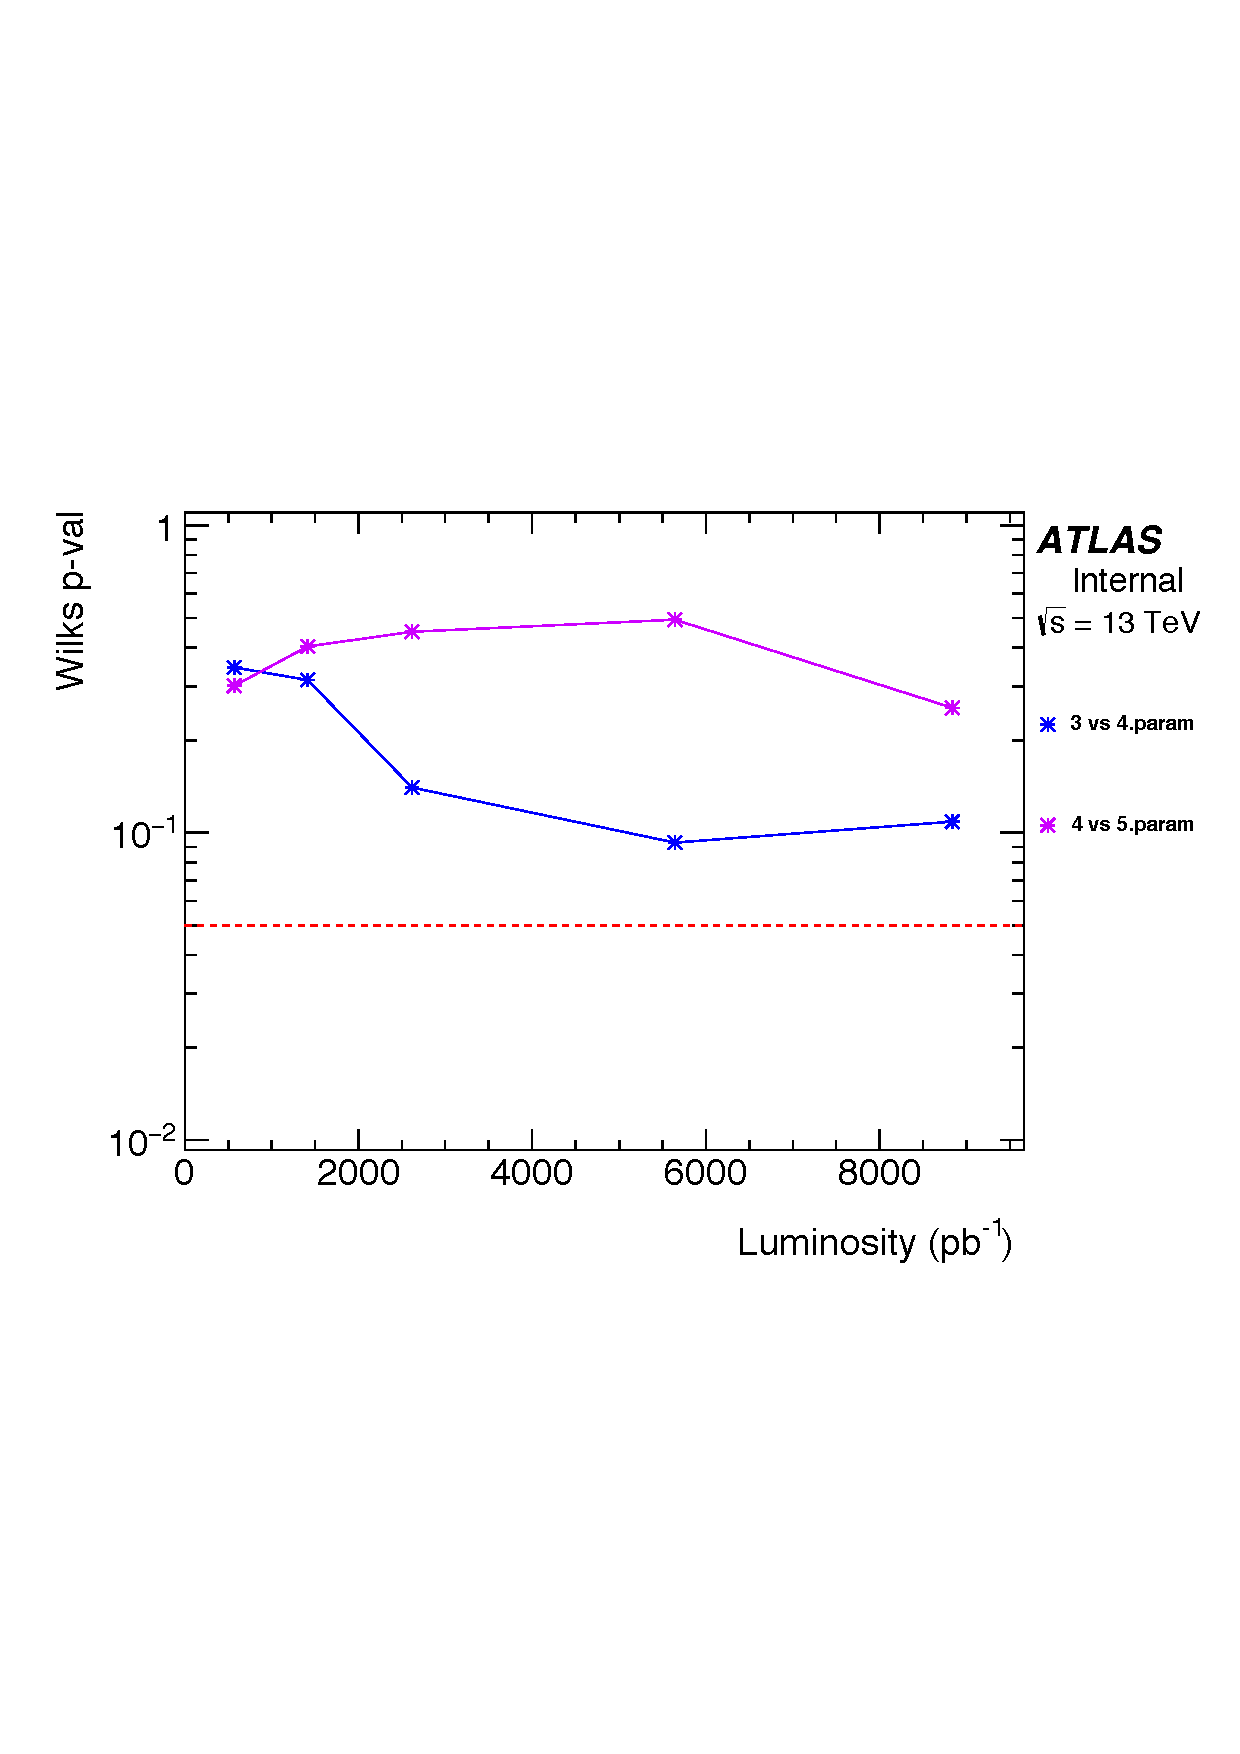
\includegraphics[width=0.8\linewidth, angle=0]{figs/Dibjet/ICHEP/bkg-WilksStat_b.pdf}}
  \end{center}
  \vspace{-1em}
  \caption
      [The Wilks' \mbox{$p$-value} as a function of luminosity for a 8.8~\ifb{} subset of the \summer{} data-set in the 2 and $\geq1$ $b$-tag category.]
      {The Wilks' \mbox{$p$-value} as a function of luminosity
        in the case that the 3 parameter dijet fit function is the nominal and the 4 parameter is the alternate (blue)
        and the case where the 4 parameter dijet fit function is the nominal and the 5 parameter is the alternate (purple)
        for a 8.8~\ifb{} subset of the \summer{} data-set in the (a) 2 and (b) $\geq1$ $b$-tag category~\cite{dibjet-ichep_conf}.
      }
  \label{fig:bkg-summer-wilks}
\end{figure}

\FloatBarrier

\clearpage
\subsection{Validation Studies: Spurious Signal}
\label{sec:bkg-summer_spusig}

If an inadequate background estimation is used fit biases can occur,
where a fit bias is defined as a difference between the true background
dijet mass spectrum and the background estimation.
Fit biases that are large compared to the statistical fluctuations of the background
can appear as false signal or could hide a true signal, the former is referred to as spurious signal.
For the di-$b$-jet search to be able to observe a new particle with confidence it is
important to demonstrate that spurious signal cannot occur.

To demonstrate that fit biases are not occurring for the 3 parameter dijet fit function
the search phase is performed on the simulated QCD dijet sample,
which is a background-only representative data-set. 
%In Section~\ref{sec:FitStudies:FitRegion}
%the dijet mass spectrum used took the square root of the
%number of effective entries as the uncertainties.
As described in Section~\ref{sec:bkg-summer_fitCR},
the simulated dijet mass spectrum contains smaller statistical fluctuations than are present in the final data-set.
Therefore, to create a dijet mass spectrum representative of the one that is expected in data 
Poisson fluctuations are applied to the scaled spectrum to create `data-like' dijet mass spectra;
Figure~\ref{fig:effEntDataLike} shows the scaled and effective entries spectra for both
$b$-tag categories overlaid with a data-like spectrum in blue.

\vspace{-0.5em}
\begin{figure}[!ht]
  \begin{center}
   \captionsetup[subfigure]{aboveskip=0pt,justification=centering}
    \subcaptionbox{2 $b$-tag}{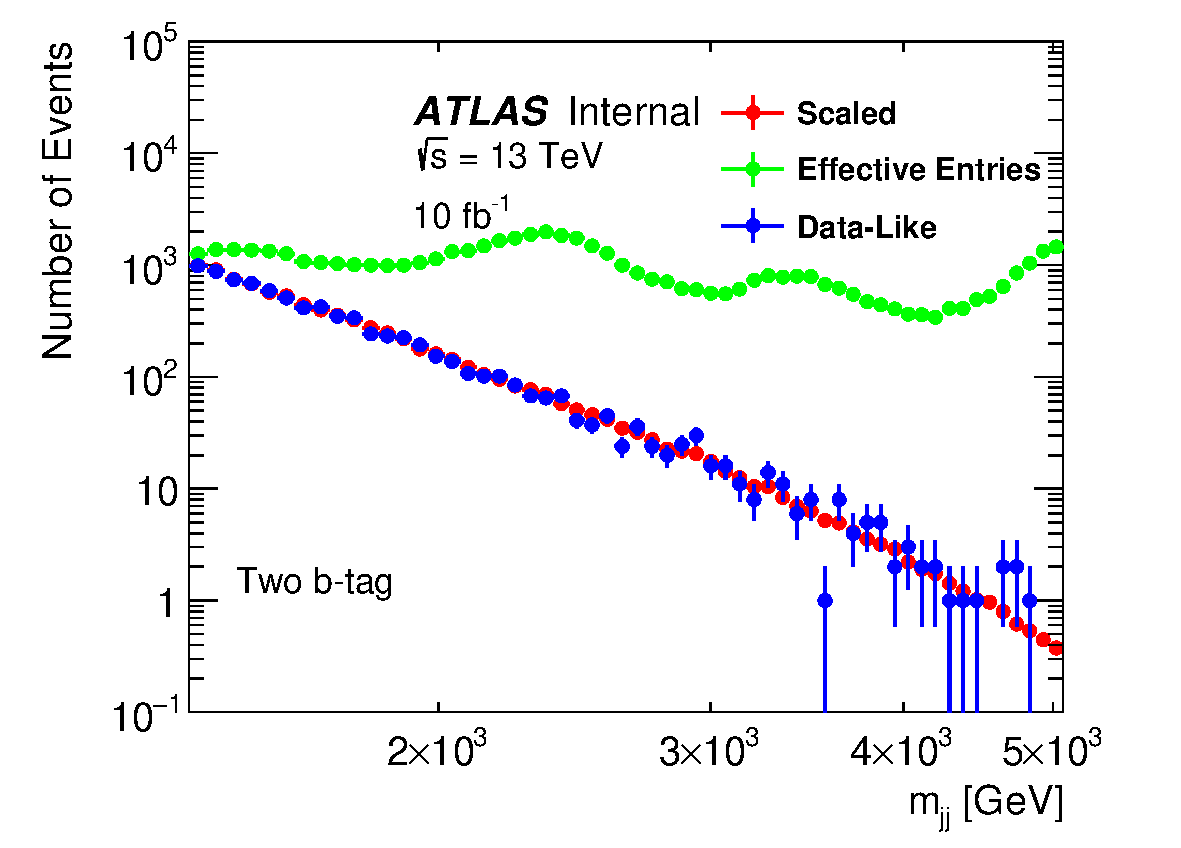
\includegraphics[width=0.48\linewidth, angle=0]{figs/Dibjet/ICHEP/SpuriousSignal/mbb_fix_8585_dataLike_effEntries_Logx_10fb.pdf}\label{fig:effEntDataLike_bb}}
    \hspace{-0.2cm}
    \subcaptionbox{$\geq$1 $b$-tag}{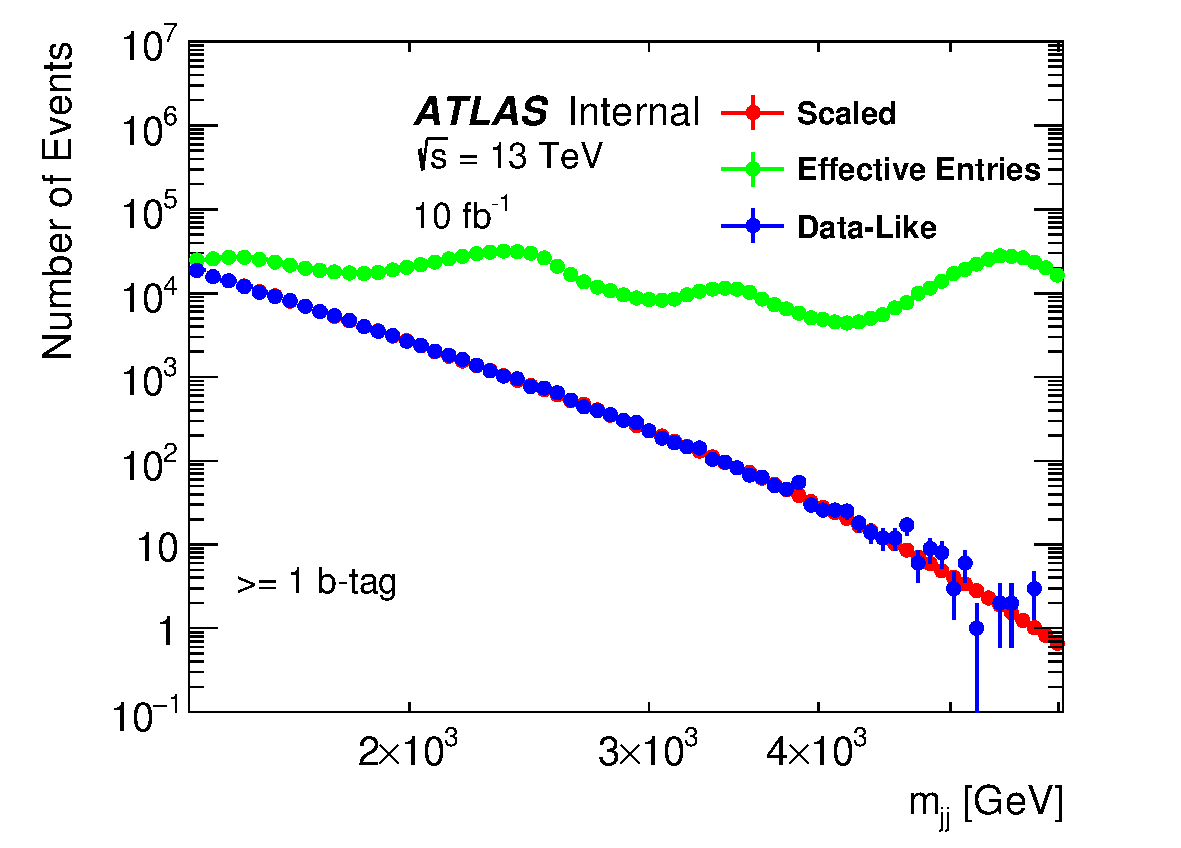
\includegraphics[width=0.48\linewidth, angle=0]{figs/Dibjet/ICHEP/SpuriousSignal/mbj_inc_fix_8585_dataLike_effEntries_Logx_10fb.pdf}\label{fig:effEntDataLike_bj}}
  \end{center}
  \vspace{-1em}
  \caption
      [The scaled and effective entries dijet mass spectra overlaid with a data-like dijet mass spectrum
        from QCD dijet simulation when the \summer{} data-set event selection has been applied.]
      {The scaled dijet mass spectrum (red) compared to the
        effective entries of the dijet mass spectrum (green)
        for the (a) 2 and (b) $\geq$1 $b$-tag categories.
        Overlaid is a data-like dijet mass spectrum (blue) created by applying Poisson fluctuations to the scaled spectrum.
        The \summer{} data-set event selection has been applied.}
  \label{fig:effEntDataLike}
\end{figure}
\vspace{-0.5em}

The search phase is then applied to the data-like dijet mass spectra
in both $b$-tag categories.
Figure~\ref{fig:DataLikeSearchPhase} shows the search phase 
using the 3 parameter dijet fit function
applied to a  data-like spectrum in both $b$-tag categories.
%The most discrepant excess is indicated by the blue lines and the \bh{} \mbox{$p$-value} of the excess is shown on the plot.
Figure~\ref{fig:DataLikeStatPlots_bh} illustrates the calculation of the \bh{} $p$-value in the search phase.
%Using a similar process, the \mbox{$p$-value} of the most discrepant deficit is calculated using the \dhunt{} test statistic
%and an overall quality of fit \mbox{$p$-value} is calculated by the $\chi^{2}$ test statistic.
For this data-like dijet mass spectrum, in the 2 $b$-tag category
the \bh{}, \dhunt{} and  $\chi^{2}$ \mbox{$p$-value} are found to be
0.57, 0.80 and 0.39 respectively.
Similarly, in the $\geq1$ $b$-tag category the
\bh{}, \dhunt{} and  $\chi^{2}$ \mbox{$p$-value}s are
0.93, 0.77 and 0.86 respectively.
Therefore, a valid background estimation has been found in both $b$-tag categories for this data-like dijet mass spectrum.


\begin{figure}[!ht]
  \begin{center}
   \captionsetup[subfigure]{aboveskip=0pt,justification=centering}
    \subcaptionbox{2 $b$-tag}{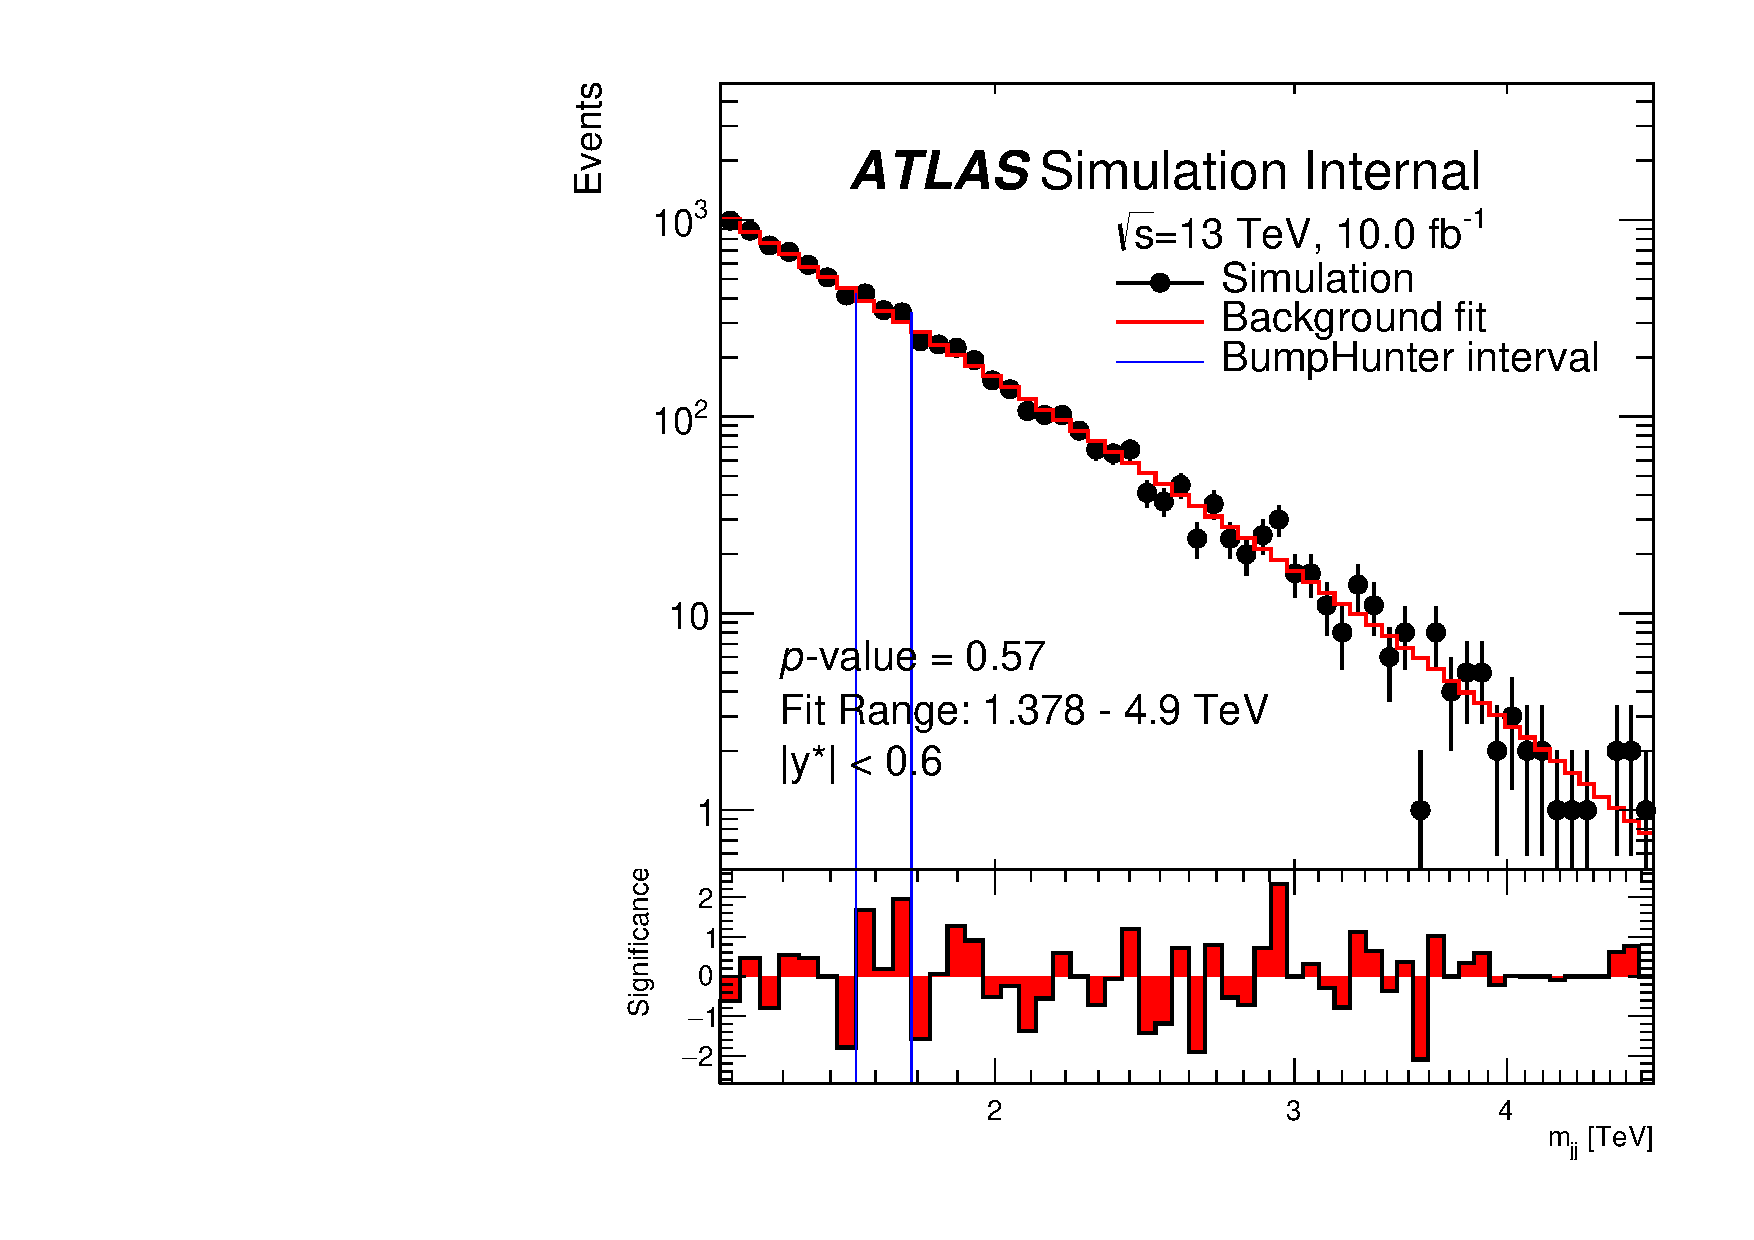
\includegraphics[width=0.47\linewidth, angle=0]{figs/Dibjet/ICHEP/SpuriousSignal/mbb_fix_8585_figure1_10fb_v10.pdf}}
    \subcaptionbox{$\geq$1 $b$-tag}{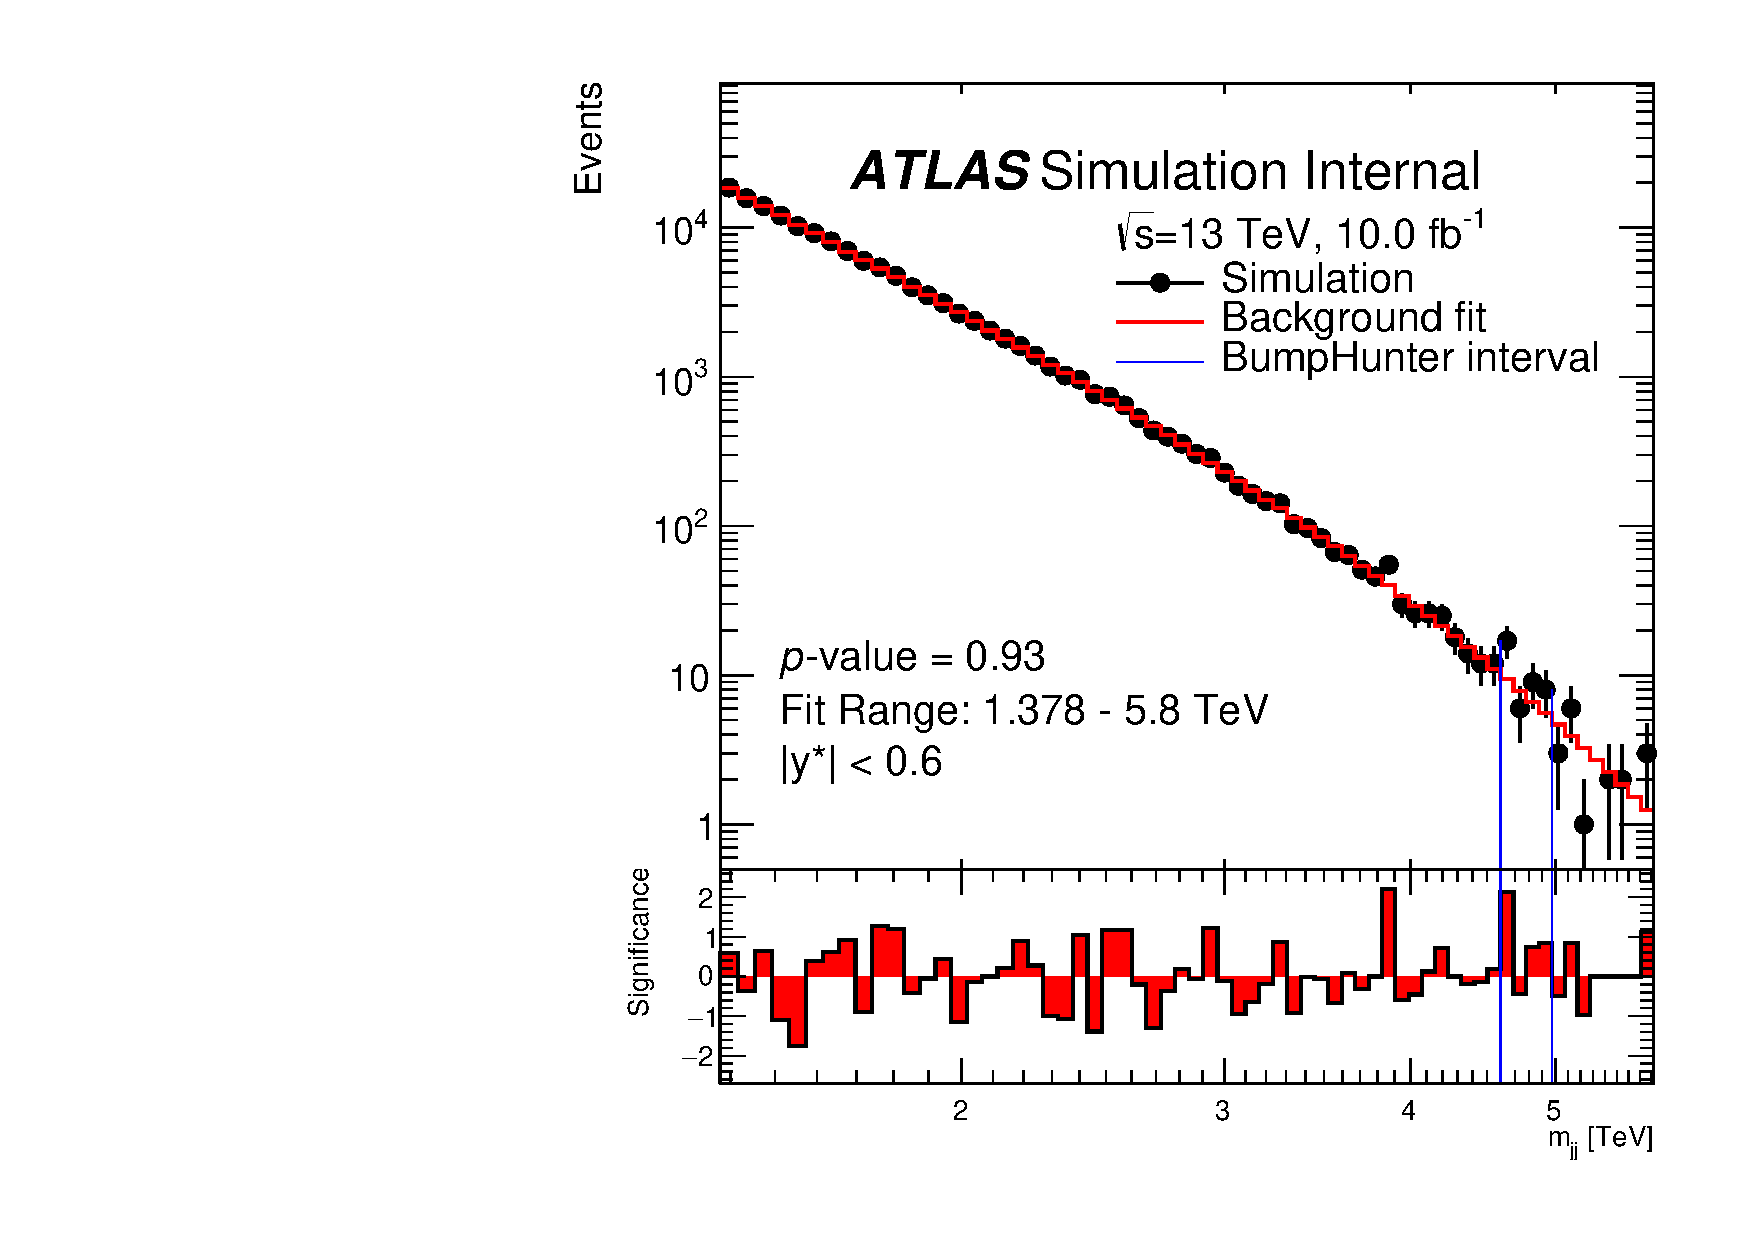
\includegraphics[width=0.47\linewidth, angle=0]{figs/Dibjet/ICHEP/SpuriousSignal/mbj_inc_fix_8585_figure1_10fb_v10.pdf}}
  \end{center}
  \vspace{-1em}
  \caption[A data-like dijet mass spectrum from QCD dijet simulation for the 2 and $\geq$1 $b$-tag
            category, fitted to using the 3 parameter dijet fit function.]
          {A data-like dijet mass spectrum from QCD dijet simulation for the (a) 2 and (b) $\geq$1 $b$-tag
            category, fitted to using the 3 parameter dijet fit function.
            The most discrepant excess as found by the \bh{} algorithm is indicated by the vertical blue lines and the \mbox{$p$-value} of this excess is printed on the plot         
            The \summer{} data-set event selection has been applied.}
  \label{fig:DataLikeSearchPhase}
%\end{figure}
%\begin{figure}[!ht]
  \begin{center}
    \captionsetup[subfigure]{aboveskip=0pt,justification=centering}
    \subcaptionbox{2 $b$-tag}{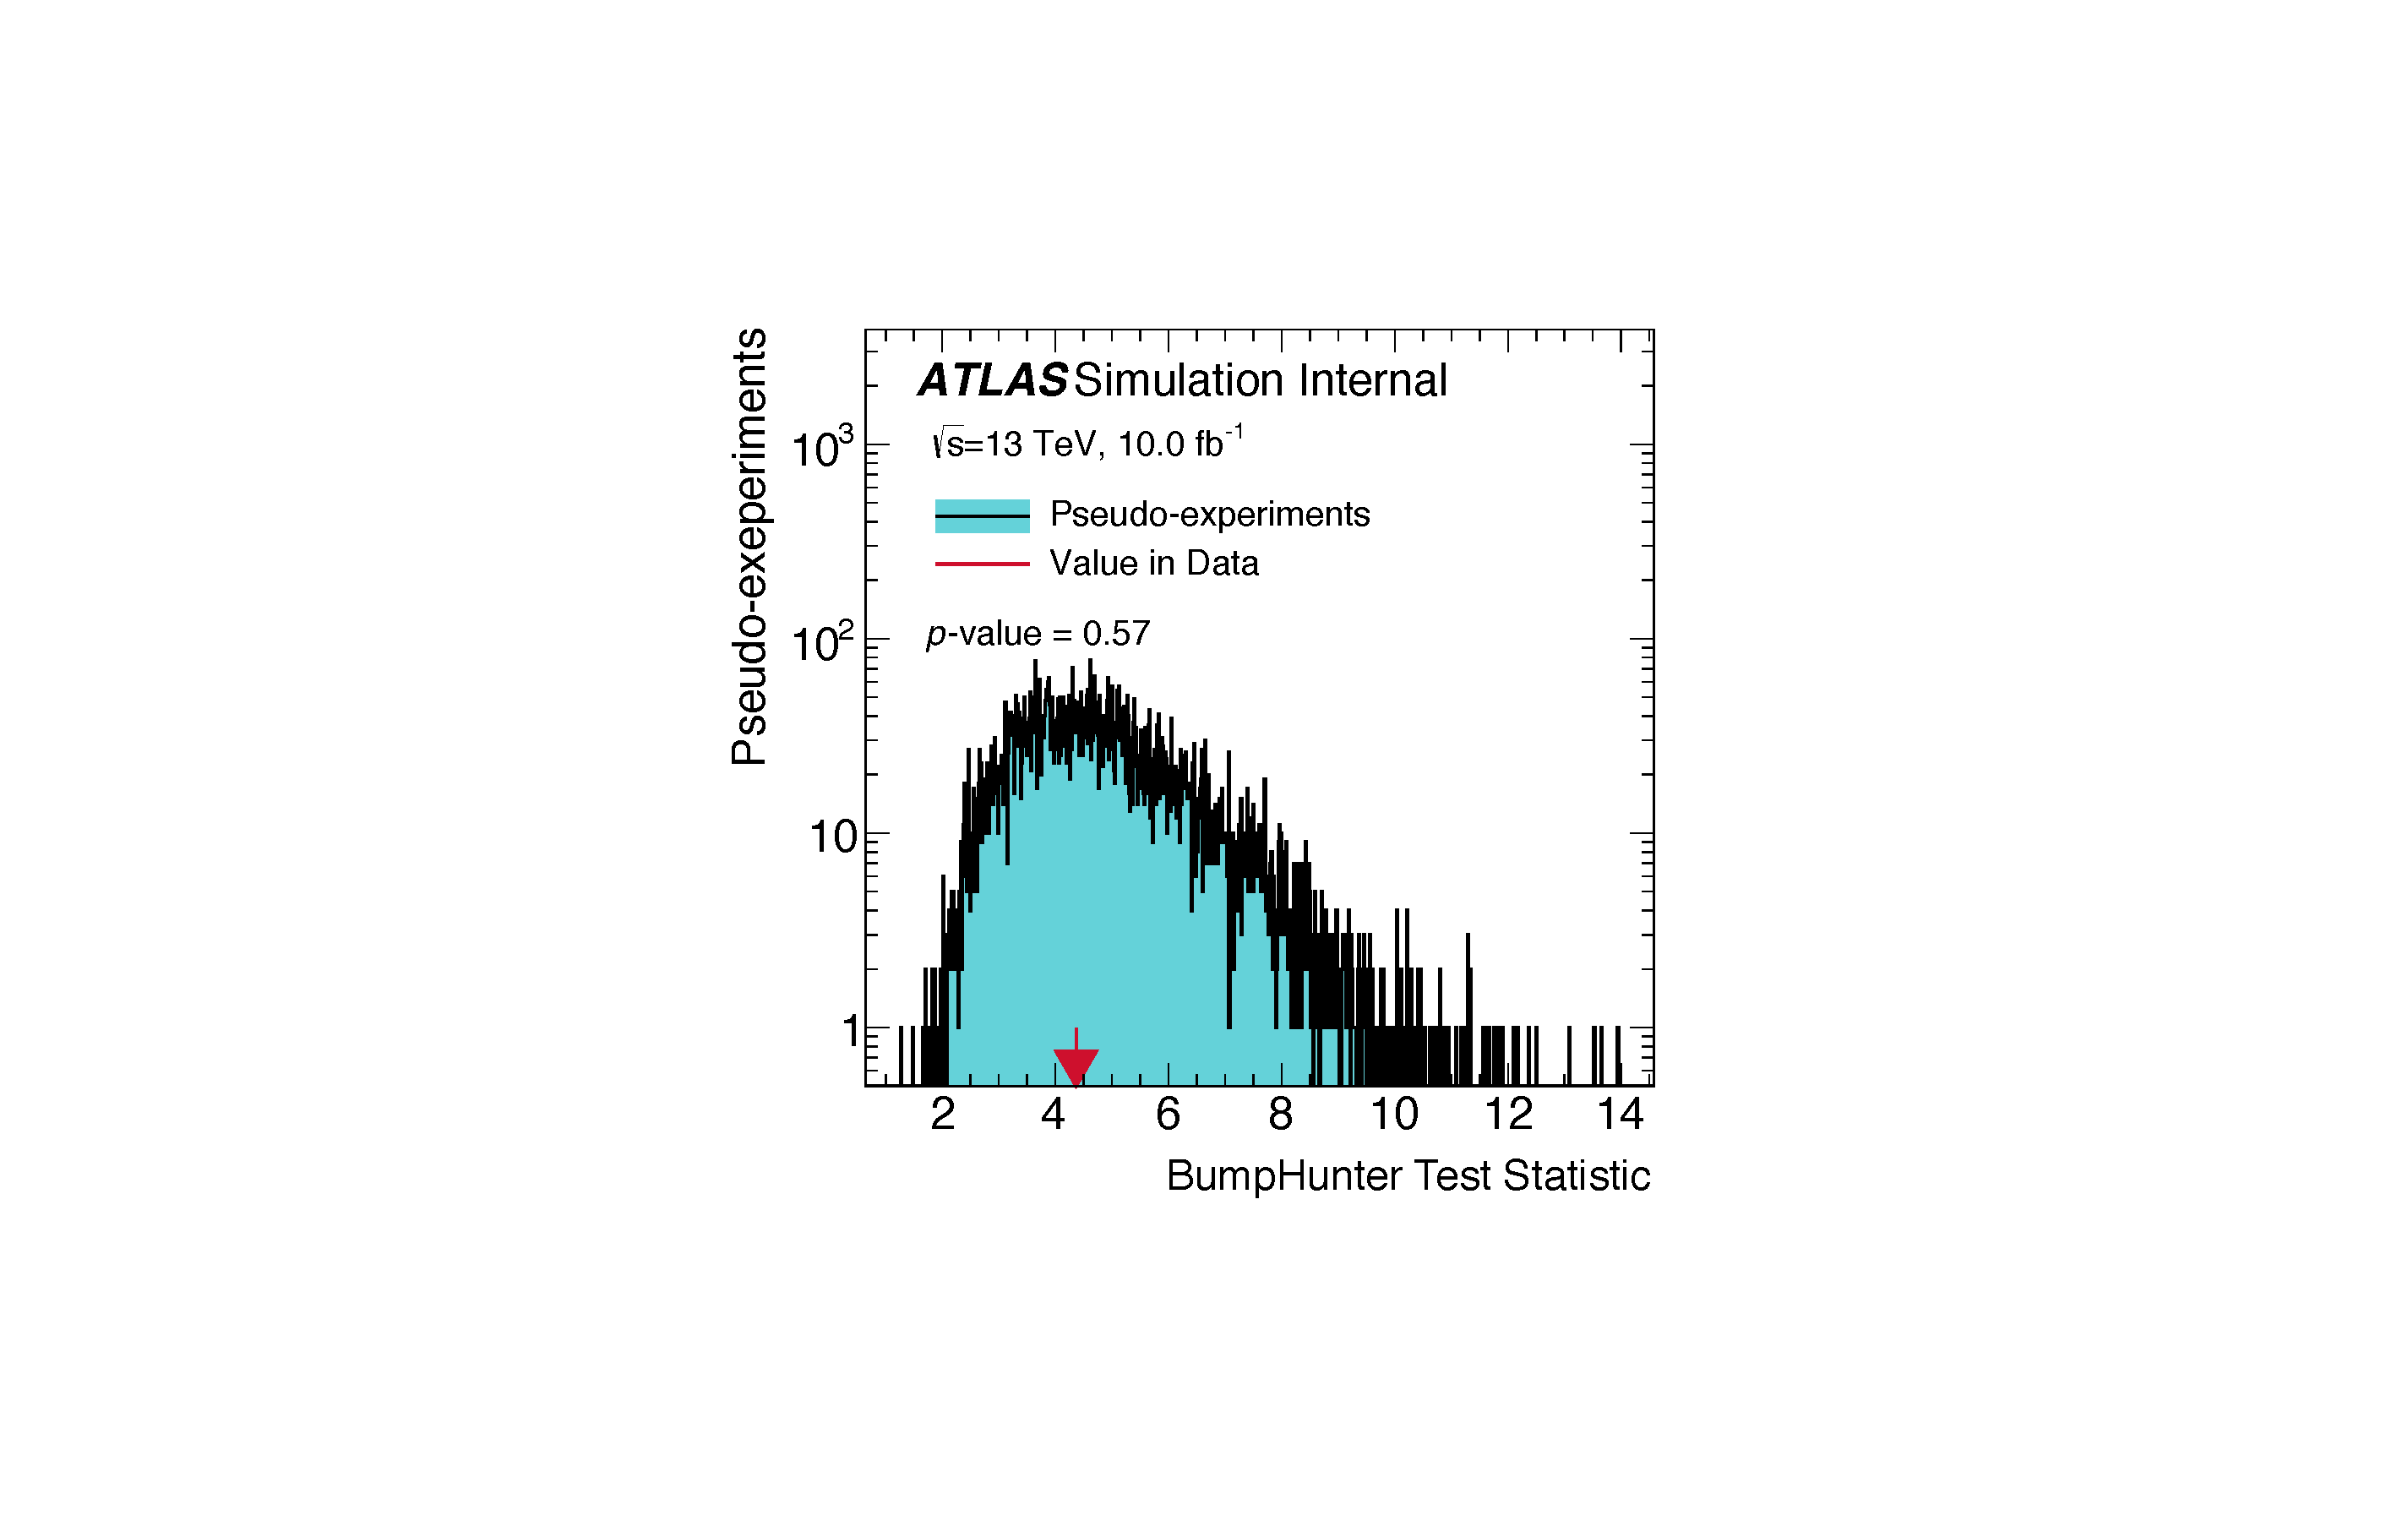
\includegraphics[width=0.47\linewidth, angle=0]{figs/Dibjet/ICHEP/SpuriousSignal/mbb_fix_8585_bumpHunterStatPlot_10fb_v10_edited.pdf}\label{fig:DataLikeBumpHunterStatPlot_bb}}
    \subcaptionbox{$\geq$1 $b$-tag}{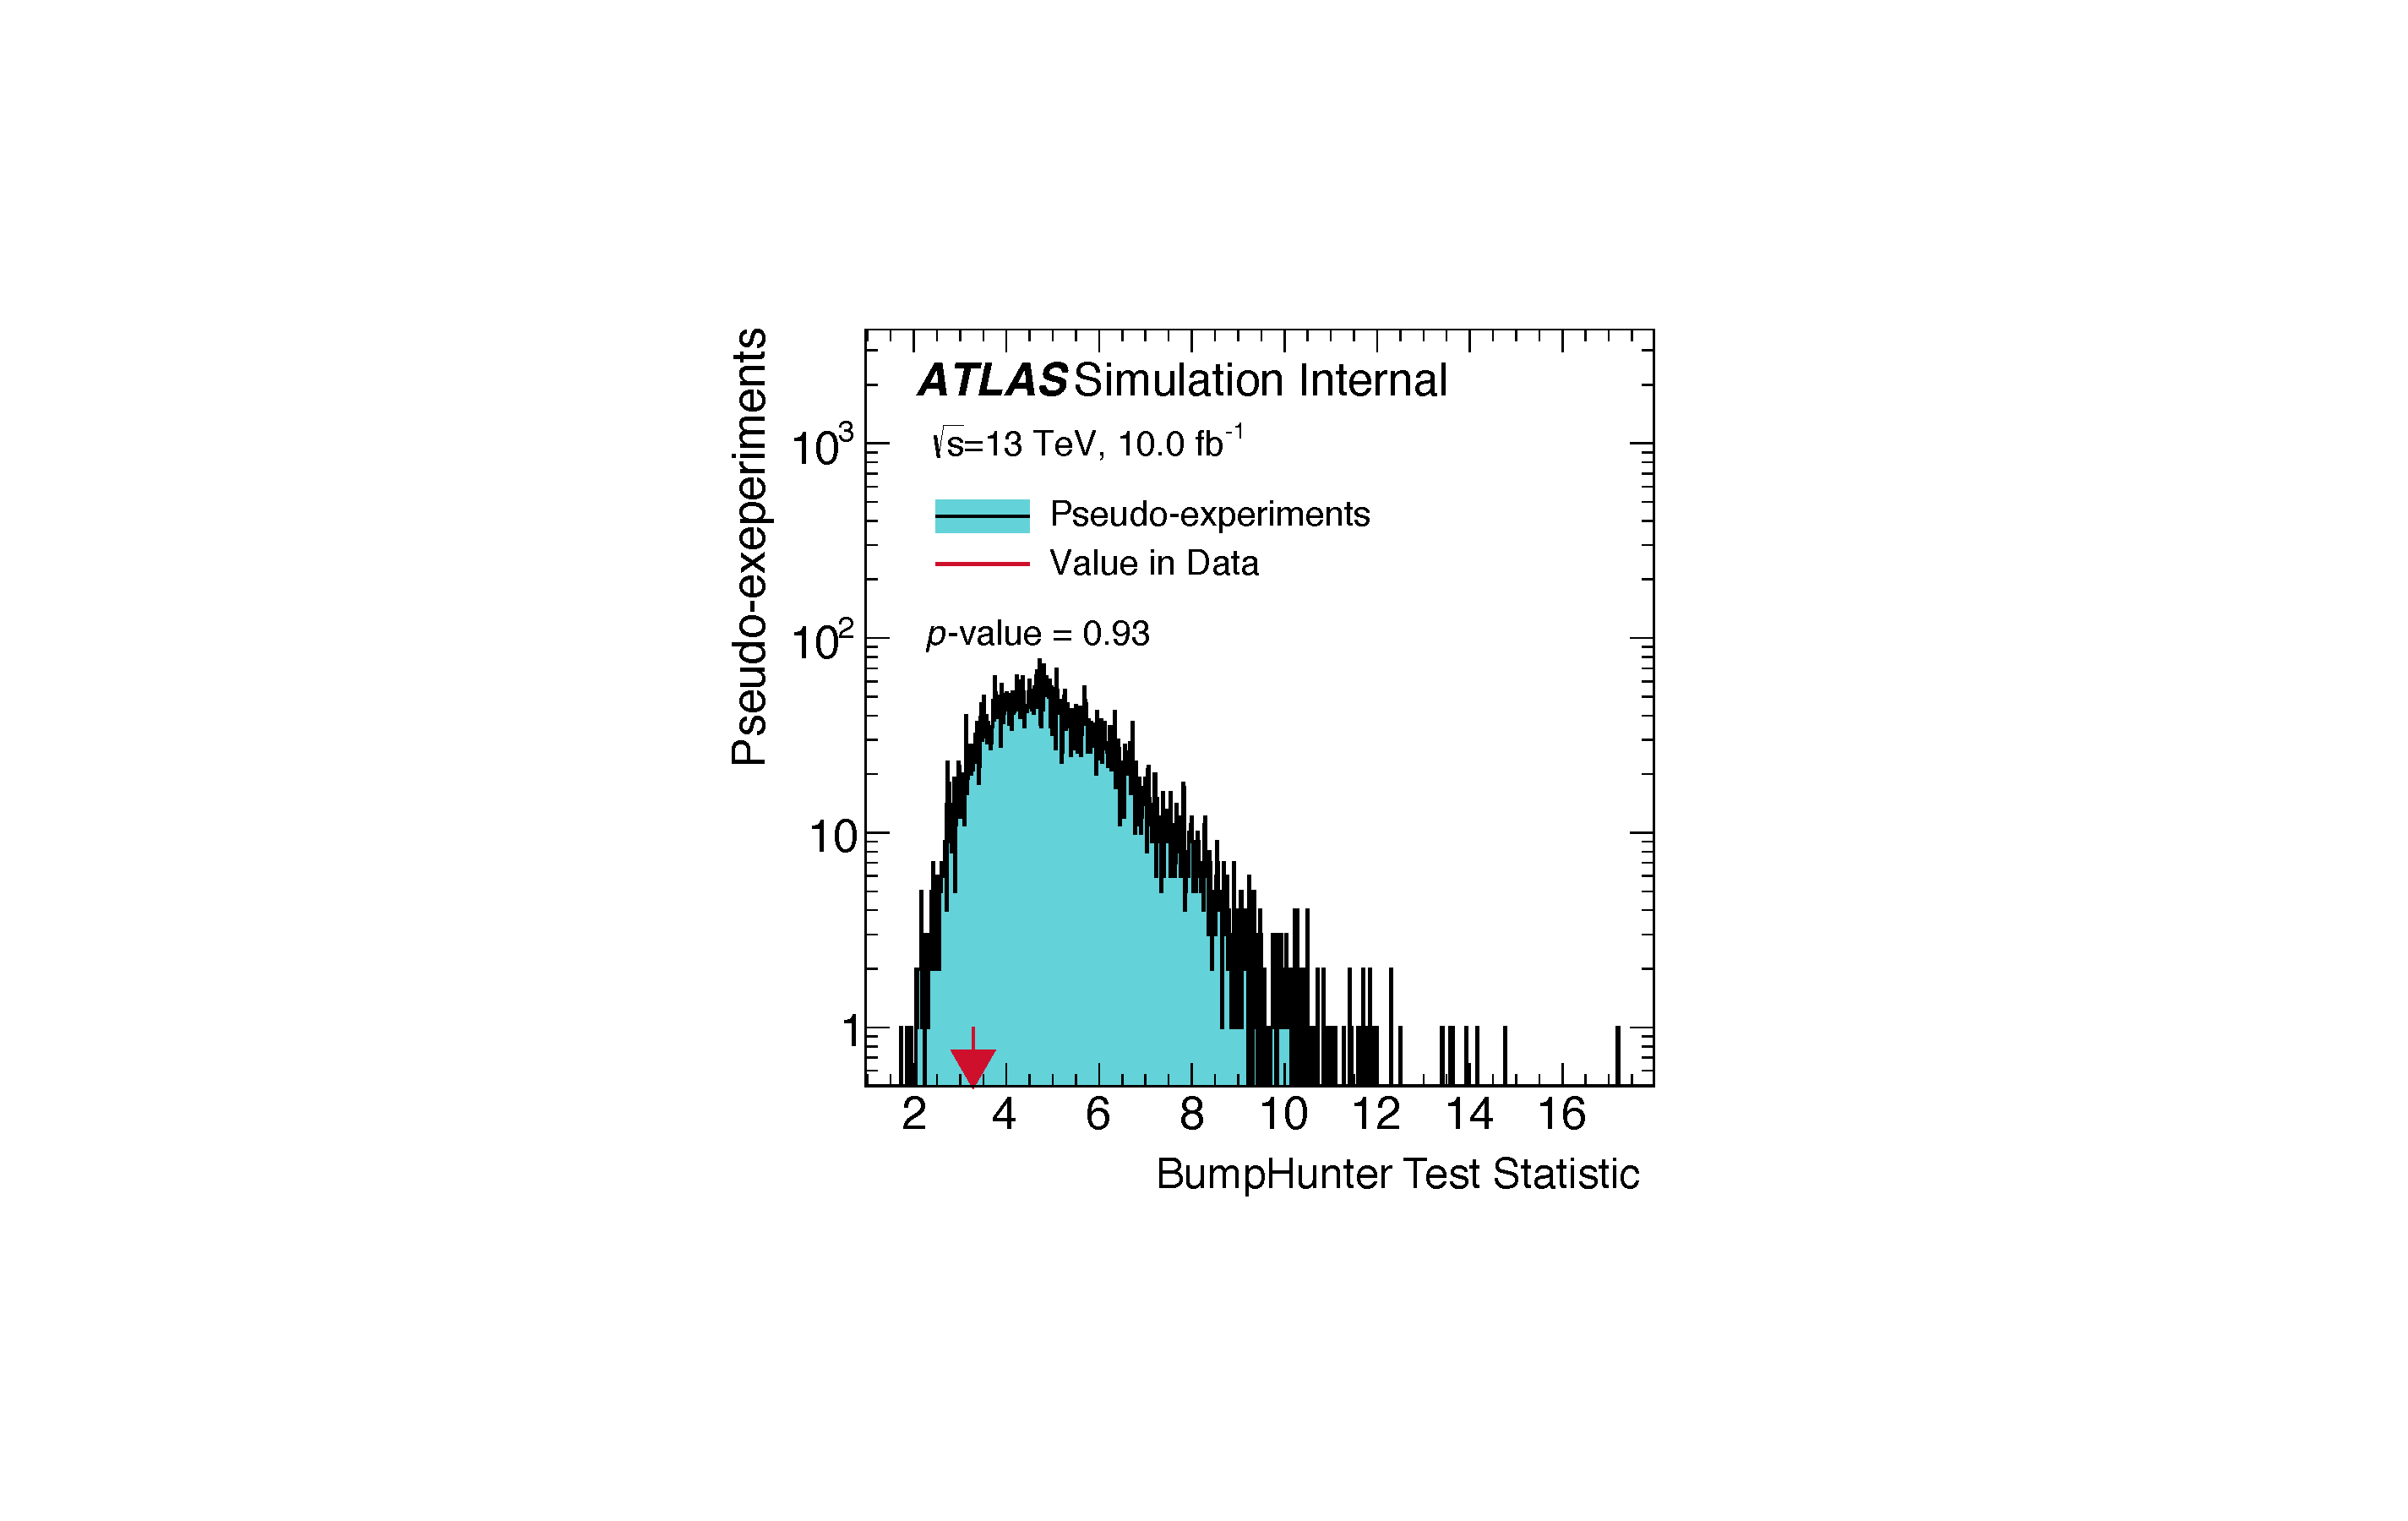
\includegraphics[width=0.47\linewidth, angle=0]{figs/Dibjet/ICHEP/SpuriousSignal/mbj_inc_fix_8585_bumpHunterStatPlot_10fb_v10_edited.pdf}\label{fig:DataLikeBumpHunterStatPlot_bj}}
  \end{center}
  \vspace{-1em}
  \caption
      [An illustration of the calculation of the \bh{} $p$-value for the search phase applied to data-like dijet mass spectra from QCD dijet simulation.
        The \summer{} data-set event selection has been applied.]
      {The observed \bh{} test statistic (red arrow) when the search phase is applied to a data-like dijet mass spectrum from QCD dijet simulation
        compared to the distribution of the \bh{} test statistic for 10,000 pseudo-experiments (blue area) taken from the background estimation for
        the (a) 2 and (b) $\geq$1 $b$-tag categories.
        The fraction of pseudo-experiments with a \bh{} test statistic greater than the observed value is the \bh{} \mbox{$p$-value}.
        The \summer{} data-set event selection has been applied.}
  \label{fig:DataLikeStatPlots_bh}
\end{figure}

However, one data-like dijet mass spectrum does not represent the full range of fluctuations that are possible.
Therefore, the search phase is applied to an ensemble of data-like dijet mass spectra,
each created using a different set of Poisson fluctuations.
Figure~\ref{fig:pValueHists}  shows the distribution of
the \bh{}, \dhunt{} and $\chi^{2}$ \mbox{$p$-value}s for 200 different data-like dijet mass spectra,
for the 2 and $\geq$1 $b$-tag category respectively.
It can be noted that there is no bias towards low \bh{} \mbox{$p$-value}s,
which shows that there is no evidence that a fit bias could cause spurious signal.
Similarly there is no bias towards low \dhunt{} \mbox{$p$-value}s,
which shows that there is no evidence that a fit bias could cause fake deficits.
Furthermore, the distribution of the $\chi^{2}$ \mbox{$p$-value}s also indicates that
there is a good fit quality observed in both $b$-tag categories.

\begin{figure}[!thb]
  \begin{center}
   \captionsetup[subfigure]{aboveskip=0pt,justification=centering}
  \subcaptionbox{\bh{} $p$-value,\\ 2 $b$-tag}{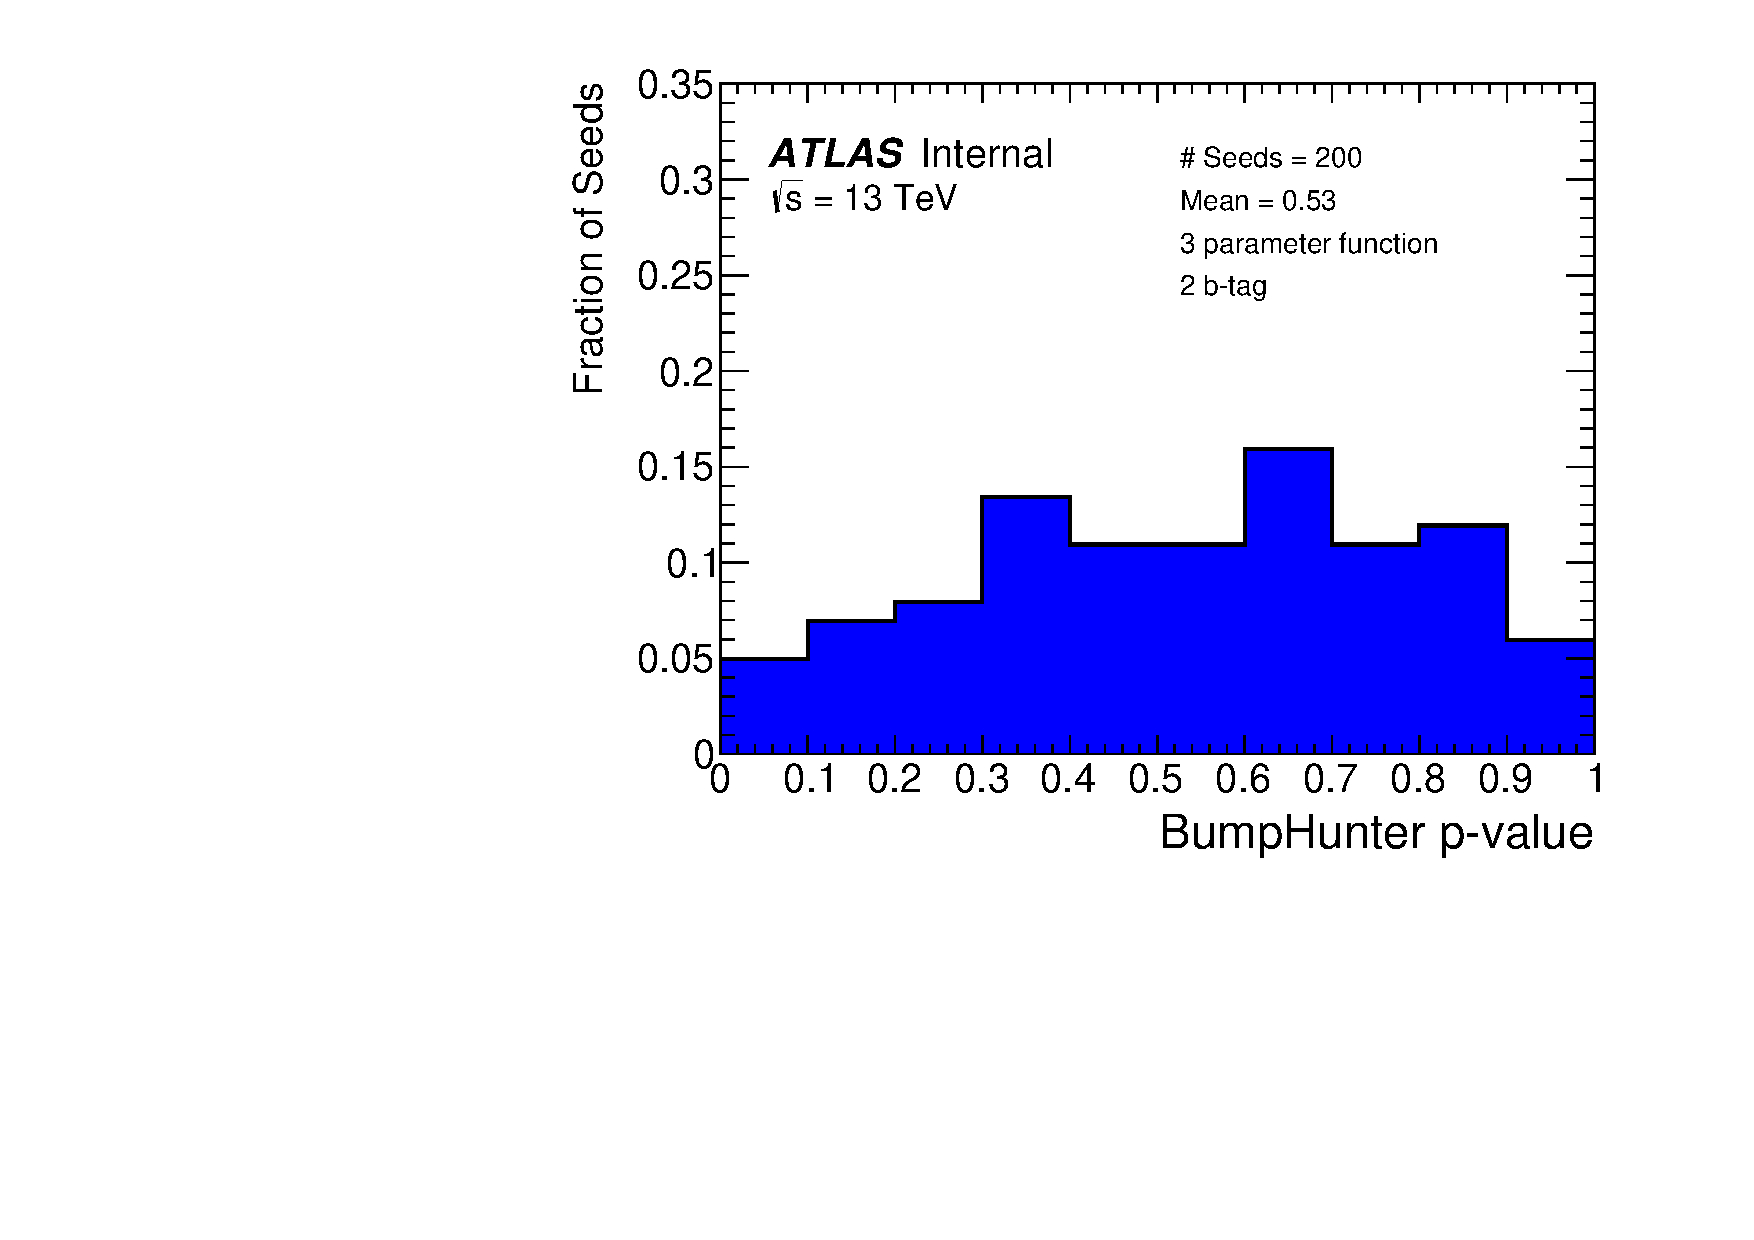
\includegraphics[width=0.45\linewidth, angle=0]{figs/Dibjet/ICHEP/SpuriousSignal/mbb_fix_8585_pValHist_bumpHunter.pdf}}
  \subcaptionbox{\bh{} $p$-value,\\ $\geq1~b$-tag}{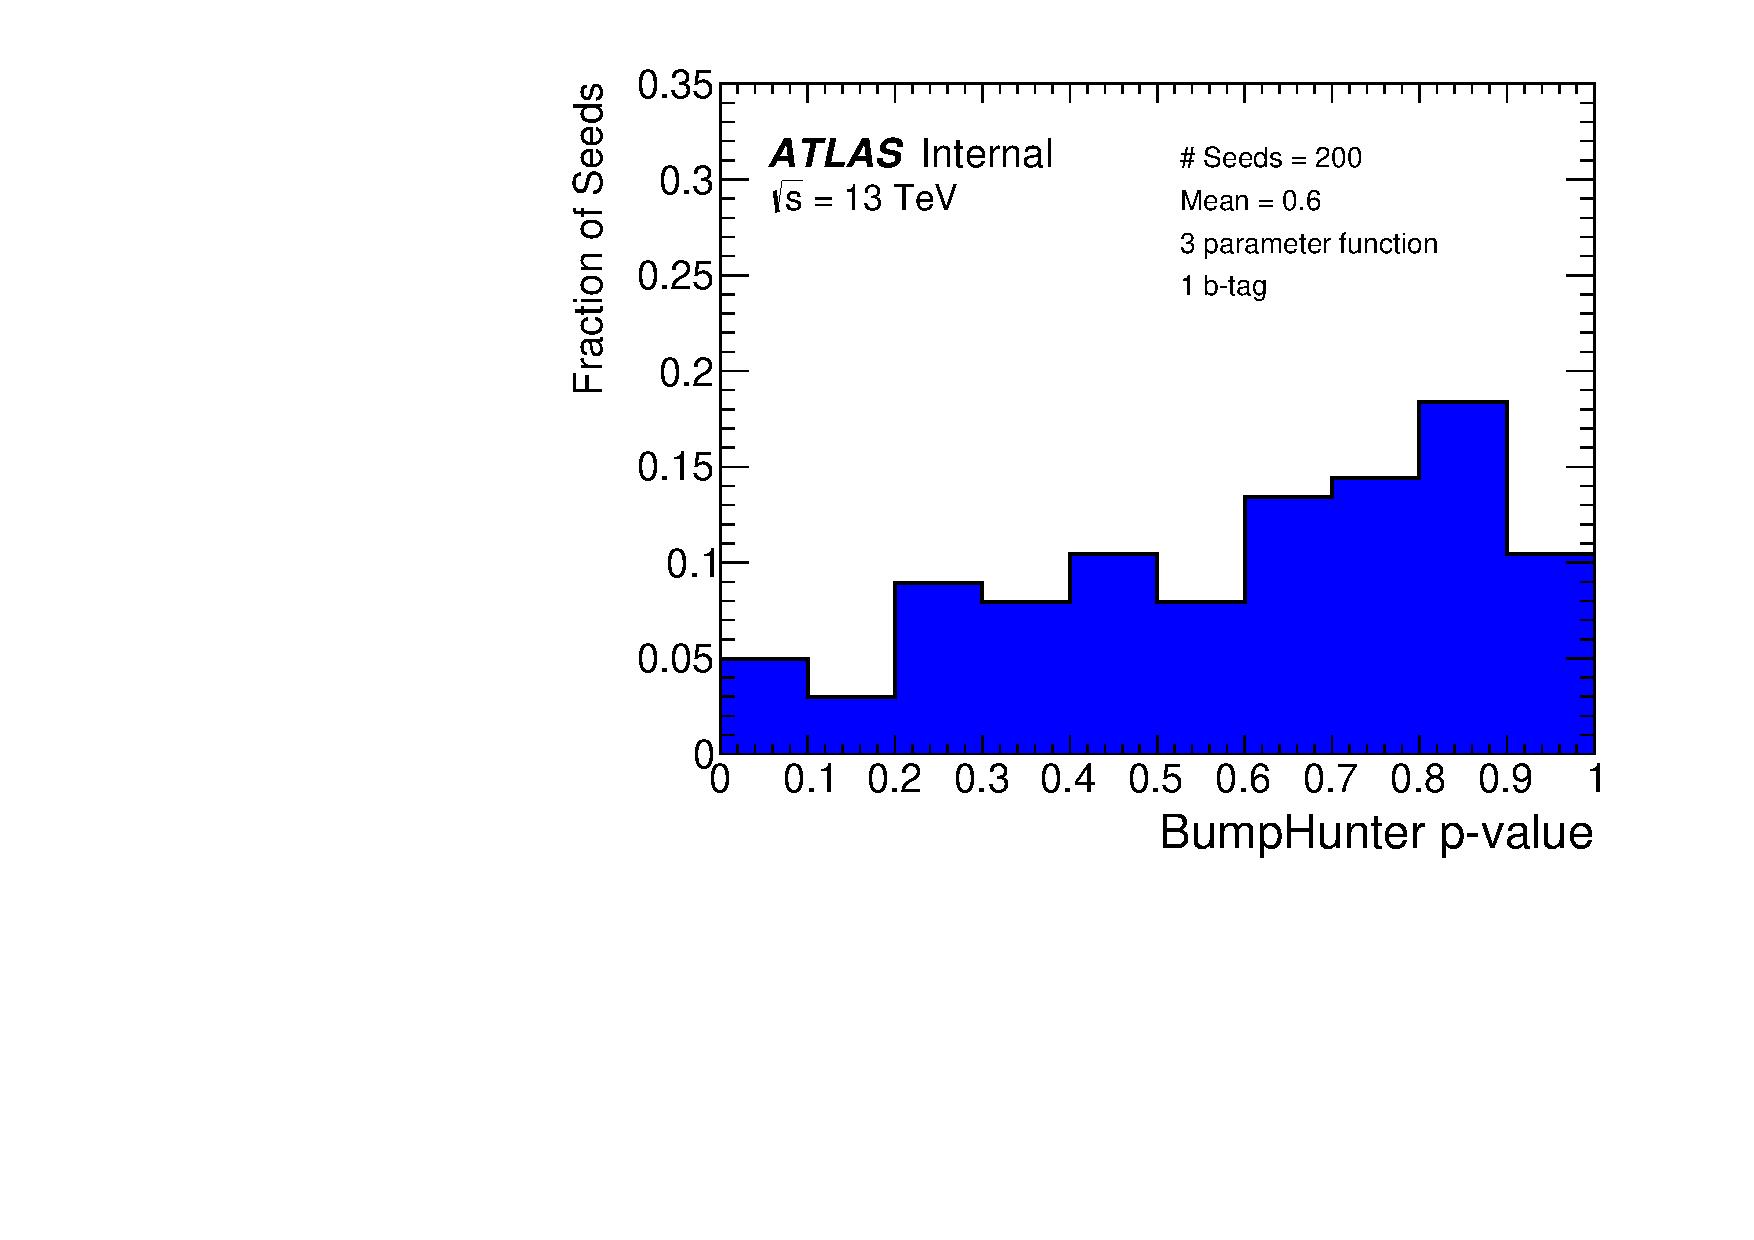
\includegraphics[width=0.45\linewidth, angle=0]{figs/Dibjet/ICHEP/SpuriousSignal/mbj_inc_fix_8585_pValHist_bumpHunter.pdf}}
  \subcaptionbox{\dhunt{} $p$-value,\\ 2 $b$-tag}{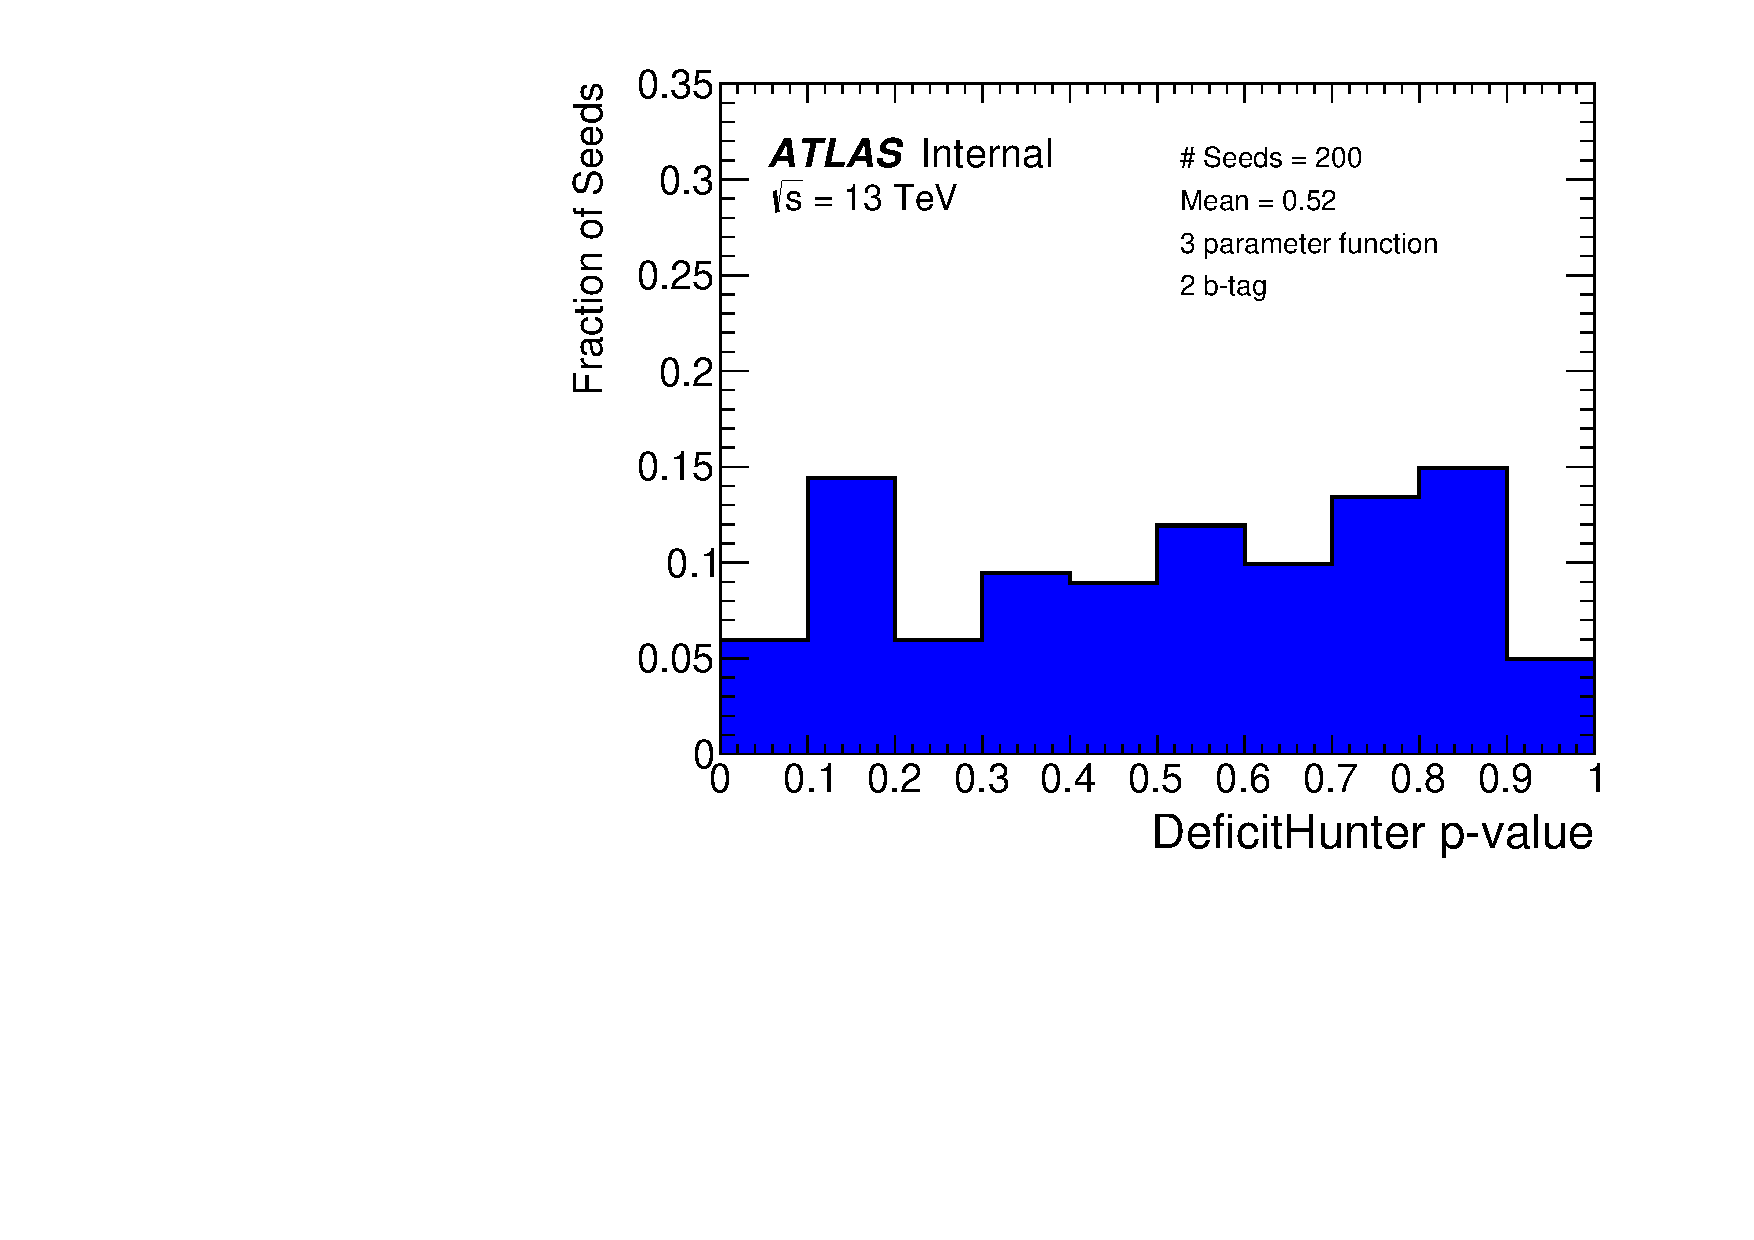
\includegraphics[width=0.45\linewidth, angle=0]{figs/Dibjet/ICHEP/SpuriousSignal/mbb_fix_8585_pValHist_deficitHunter.pdf}}
  \subcaptionbox{\dhunt{} $p$-value,\\ $\geq1~b$-tag}{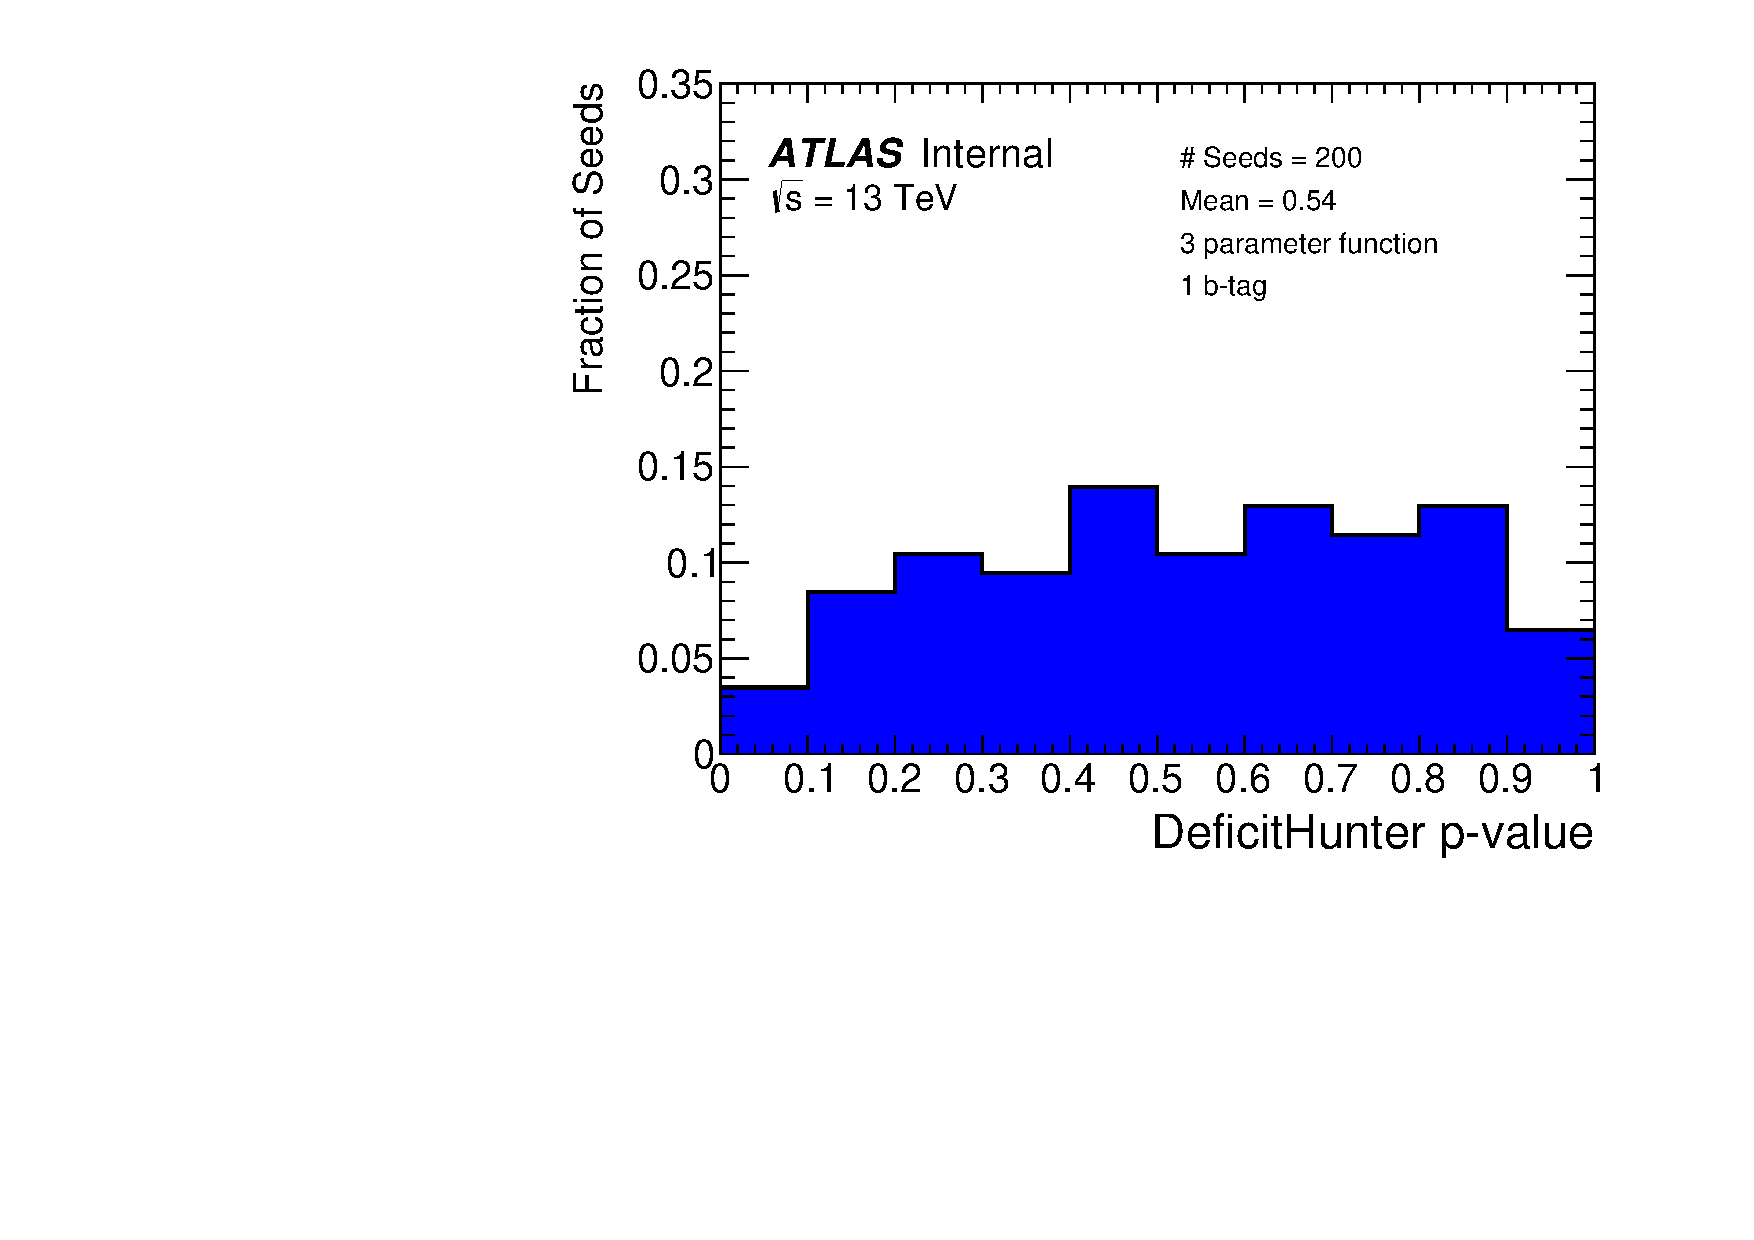
\includegraphics[width=0.45\linewidth, angle=0]{figs/Dibjet/ICHEP/SpuriousSignal/mbj_inc_fix_8585_pValHist_deficitHunter.pdf}}
  \subcaptionbox{$\chi^{2}$ $p$-value,\\ 2 $b$-tag}{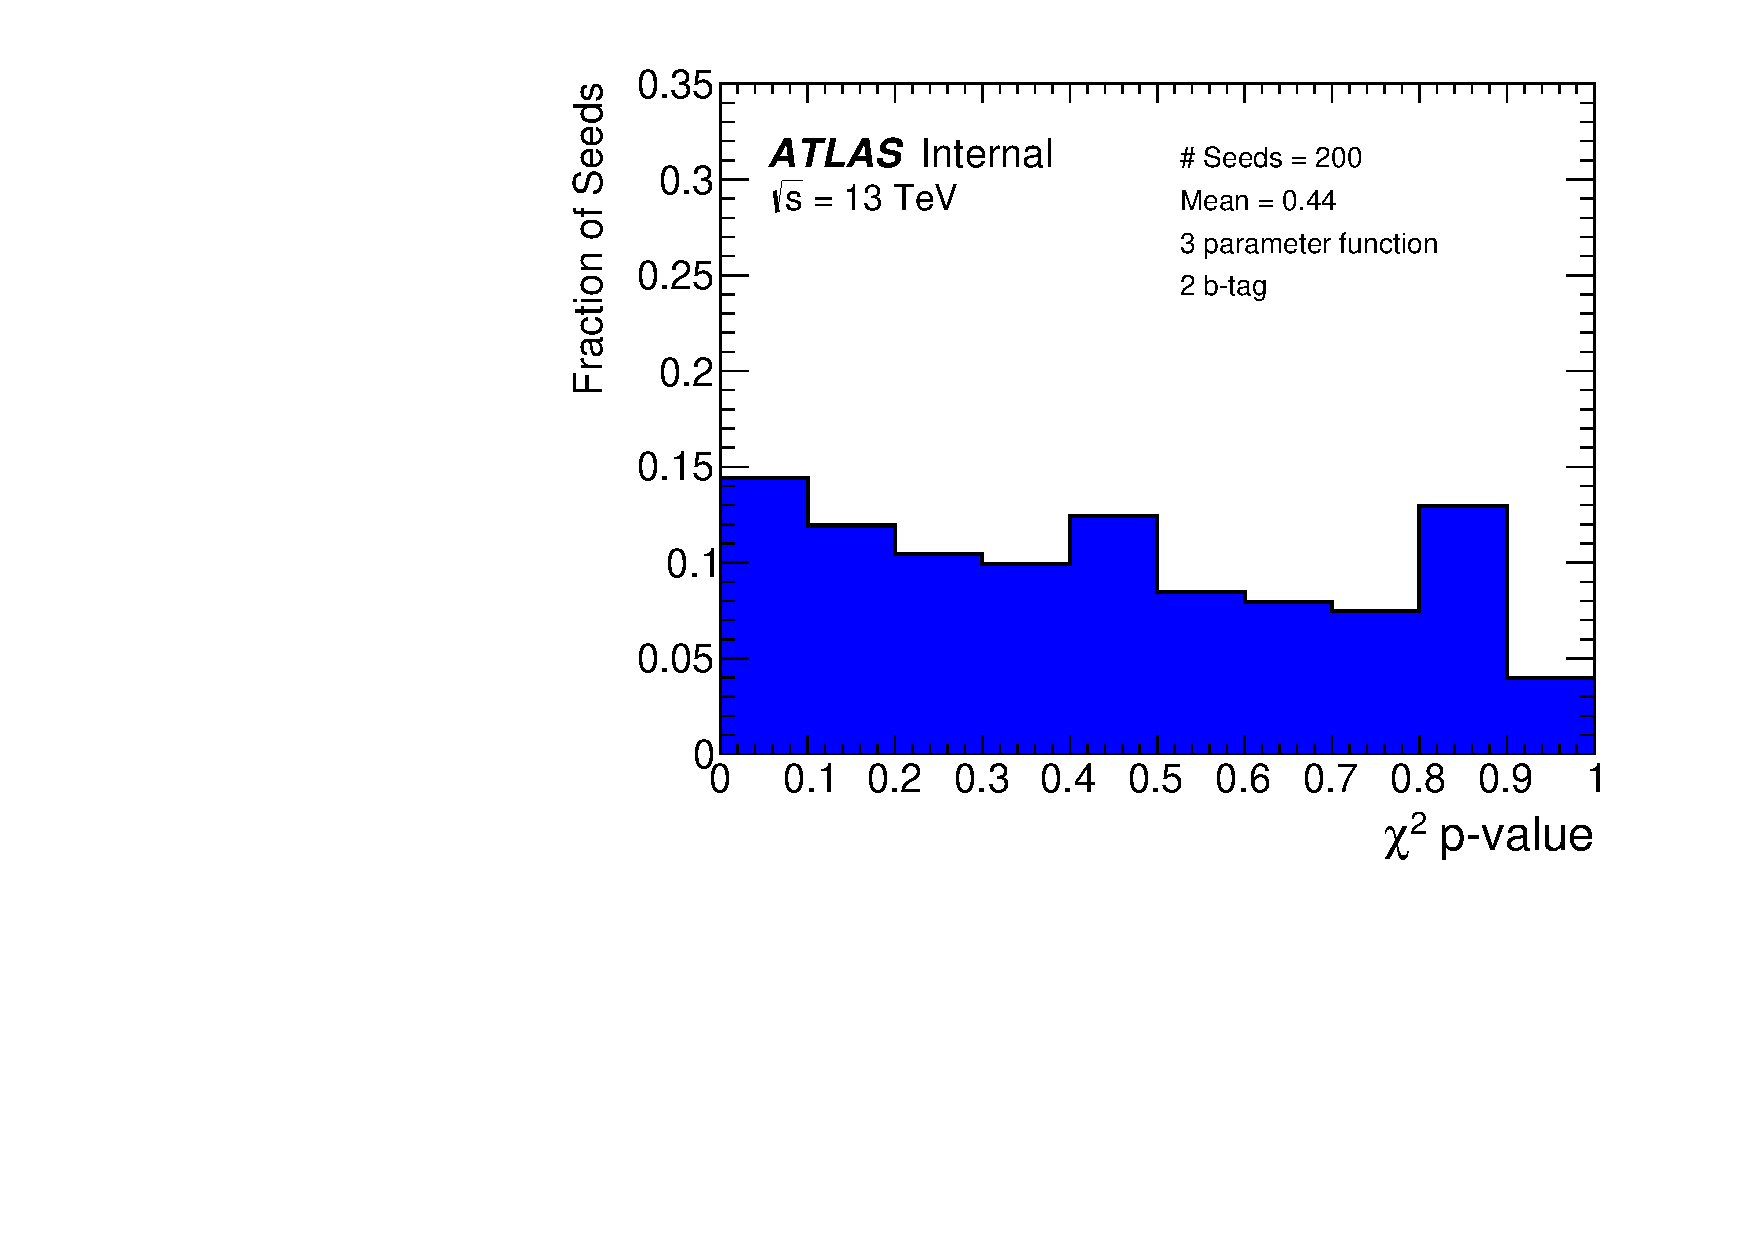
\includegraphics[width=0.45\linewidth, angle=0]{figs/Dibjet/ICHEP/SpuriousSignal/mbb_fix_8585_pValHist_chi2.pdf}}
  \subcaptionbox{$\chi^{2}$ $p$-value,\\ $\geq1~b$-tag}{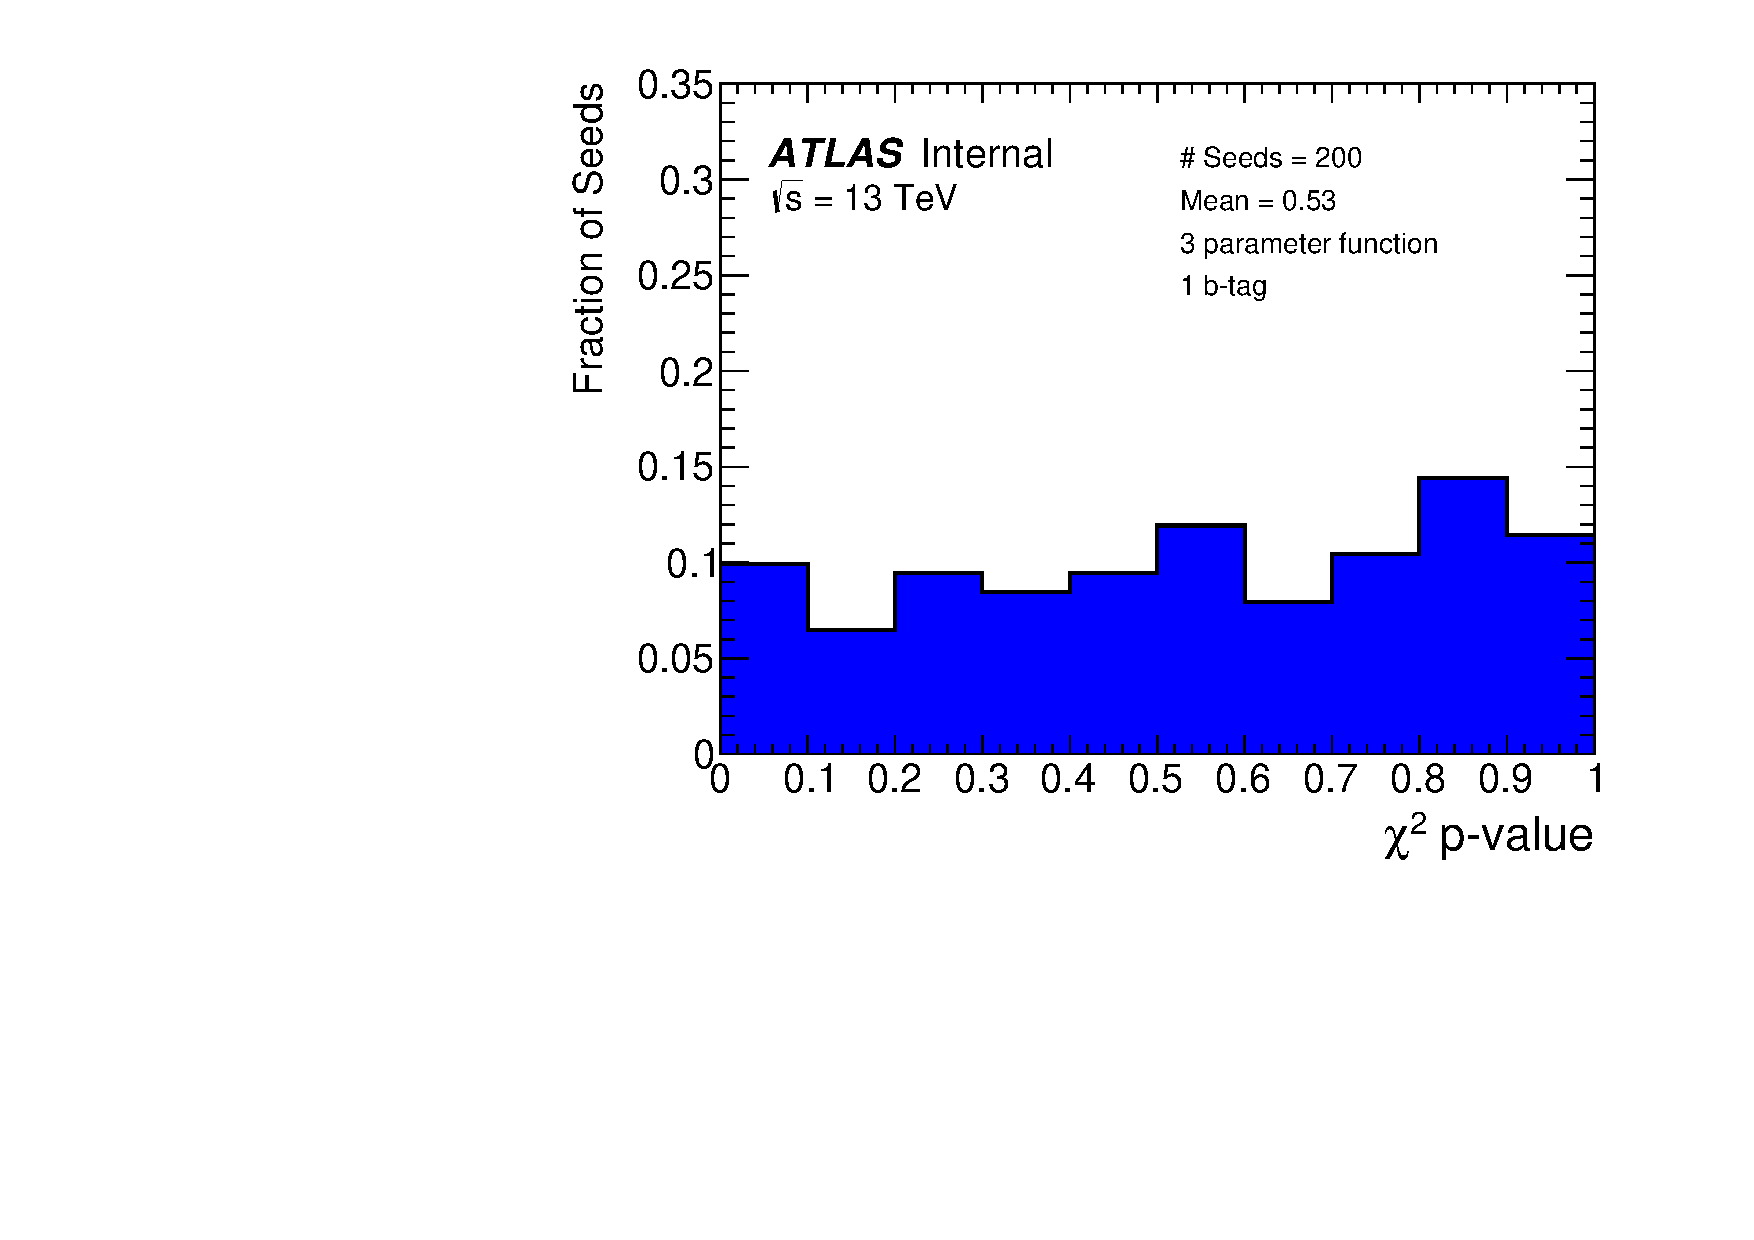
\includegraphics[width=0.45\linewidth, angle=0]{figs/Dibjet/ICHEP/SpuriousSignal/mbj_inc_fix_8585_pValHist_chi2.pdf}}
  \end{center}
  \vspace{-1em}
  \caption
      [The normalised distributions of \bh{}, \dhunt{} and $\chi^{2}$  \mbox{$p$-value}s for
        the search phase performed on 200 data-like dijet mass spectra from QCD dijet simulation.
        The \summer{} data-set event selection has been applied.]
      {The normalised distributions of \bh{} (top row),  \dhunt{} (middle row) and $\chi^{2}$ (bottom row) \mbox{$p$-value}s for
        the search phase using the 3 parameter dijet fit function performed on
        200 data-like dijet mass spectra from QCD dijet simulation
        for the 2 $b$-tag category (left column) and $\geq1~b$-tag category (right column).
        The \summer{} data-set event selection has been applied.
        \label{fig:pValueHists}}

\end{figure}

%Hence, it is concluded that the 3 parameter dijet fit function
%provides a valid background estimation for the background-only representative data-set
%and that fit biases and spurious signal cannot occur.

%Similar tests were performed for the 4 parameter dijet fit function but are not presented here because,
%as shown in Section~\ref{sec:bkg-summer_global},
%the 3 parameter dijet fit function is chosen in both categories for this data-set.
\vspace{-0.25em}

\subsection{Validation Studies: Signal Injection}
\label{sec:bkg-summer_sigInj}

\vspace{-0.25em}
If an excess with a  \bh{} $p$-value $<$ 0.01 is observed then the background estimation is
performed again with an exclusion region applied.
The exclusion region is defined as the mass range of the excess with one additional bin on the low mass side.
The fit ignores all bins in the exclusion region, meaning that signal induced fit biases are removed.

It has been shown in previous iterations of the inclusive dijet and di-$b$-jet searches at ATLAS~\cite{dijet-mori16_paper,dibjet-mori16_paper} that,
using the region exclusion procedure, the 3 parameter dijet fit function is able to describe a data-like dijet mass spectrum
taken from a simulated QCD dijet sample when a signal has been injected.
This is because the parameters of the 3 parameter dijet fit function are highly constrained by the QCD background
and the region exclusion procedure will remove any signal induced fit bias cause by a large signal.
Hence, it is concluded that the search phase using the 3 parameter dijet fit function is robust against the presence of signal.

To conclude the search phase validation studies for the \summer{} data-set analysis,
it has been shown that the 3 parameter dijet fit function has a
sufficient number of parameters to provide an adequate background
and that there is no evidence that spurious signal can occur.
It is also known that the search phase using the 3 parameter dijet fit function
will not produce large signal induced fit biases.
Hence, the 3 parameter dijet fit function
provides a valid background estimation in both $b$-tag categories.

\subsection{Search Phase Results}
\label{sec:bkg-summer_results}

\vspace{-0.5em}
Figure~\ref{fig:bkg-summer_searchPhase} shows the dijet mass spectrum of the
\summer{} data-set and the background estimate created using the 3 parameter dijet fit function
in the 2 and $\geq1$ $b$-tag categories.
The upper panel shows the data compared to the background estimation,
in addition the benchmark signal models with enhanced cross sections have been overlaid.
The lower panel shows the significance of the difference between the data and background estimate.

In both cases the \bh{} algorithm has identified the most discrepant excess indicated
in the figure using vertical blue lines;
the \bh{} \mbox{$p$-value} has been calculated using 10,000 pseudo-experiments.
The \bh{} \mbox{$p$-value} is 0.60 in the 2 $b$-tag category
and 0.44 in the $\geq1$ $b$-tag category;
this shows that no significant excess is found in either \mbox{$b$-tag} category and it is therefore concluded
that there is no evidence of a BSM resonance in the \summer{} data-set.
As no significant excess is found, limits on the benchmark signal models are set using the \summer{} data-set,
which will be shown in Chapter~\ref{sec:lim}.


\begin{figure}[!htb]
  \begin{center}
    \captionsetup[subfigure]{aboveskip=0pt,justification=centering}
   \subcaptionbox{2 $b$-tag\vspace{1em}}{\includegraphics[width=0.65\linewidth, angle=0]{figs/Dibjet/ICHEP/bkg-SearchPhase_bb.png}}

   \subcaptionbox{$\geq$1 $b$-tag}{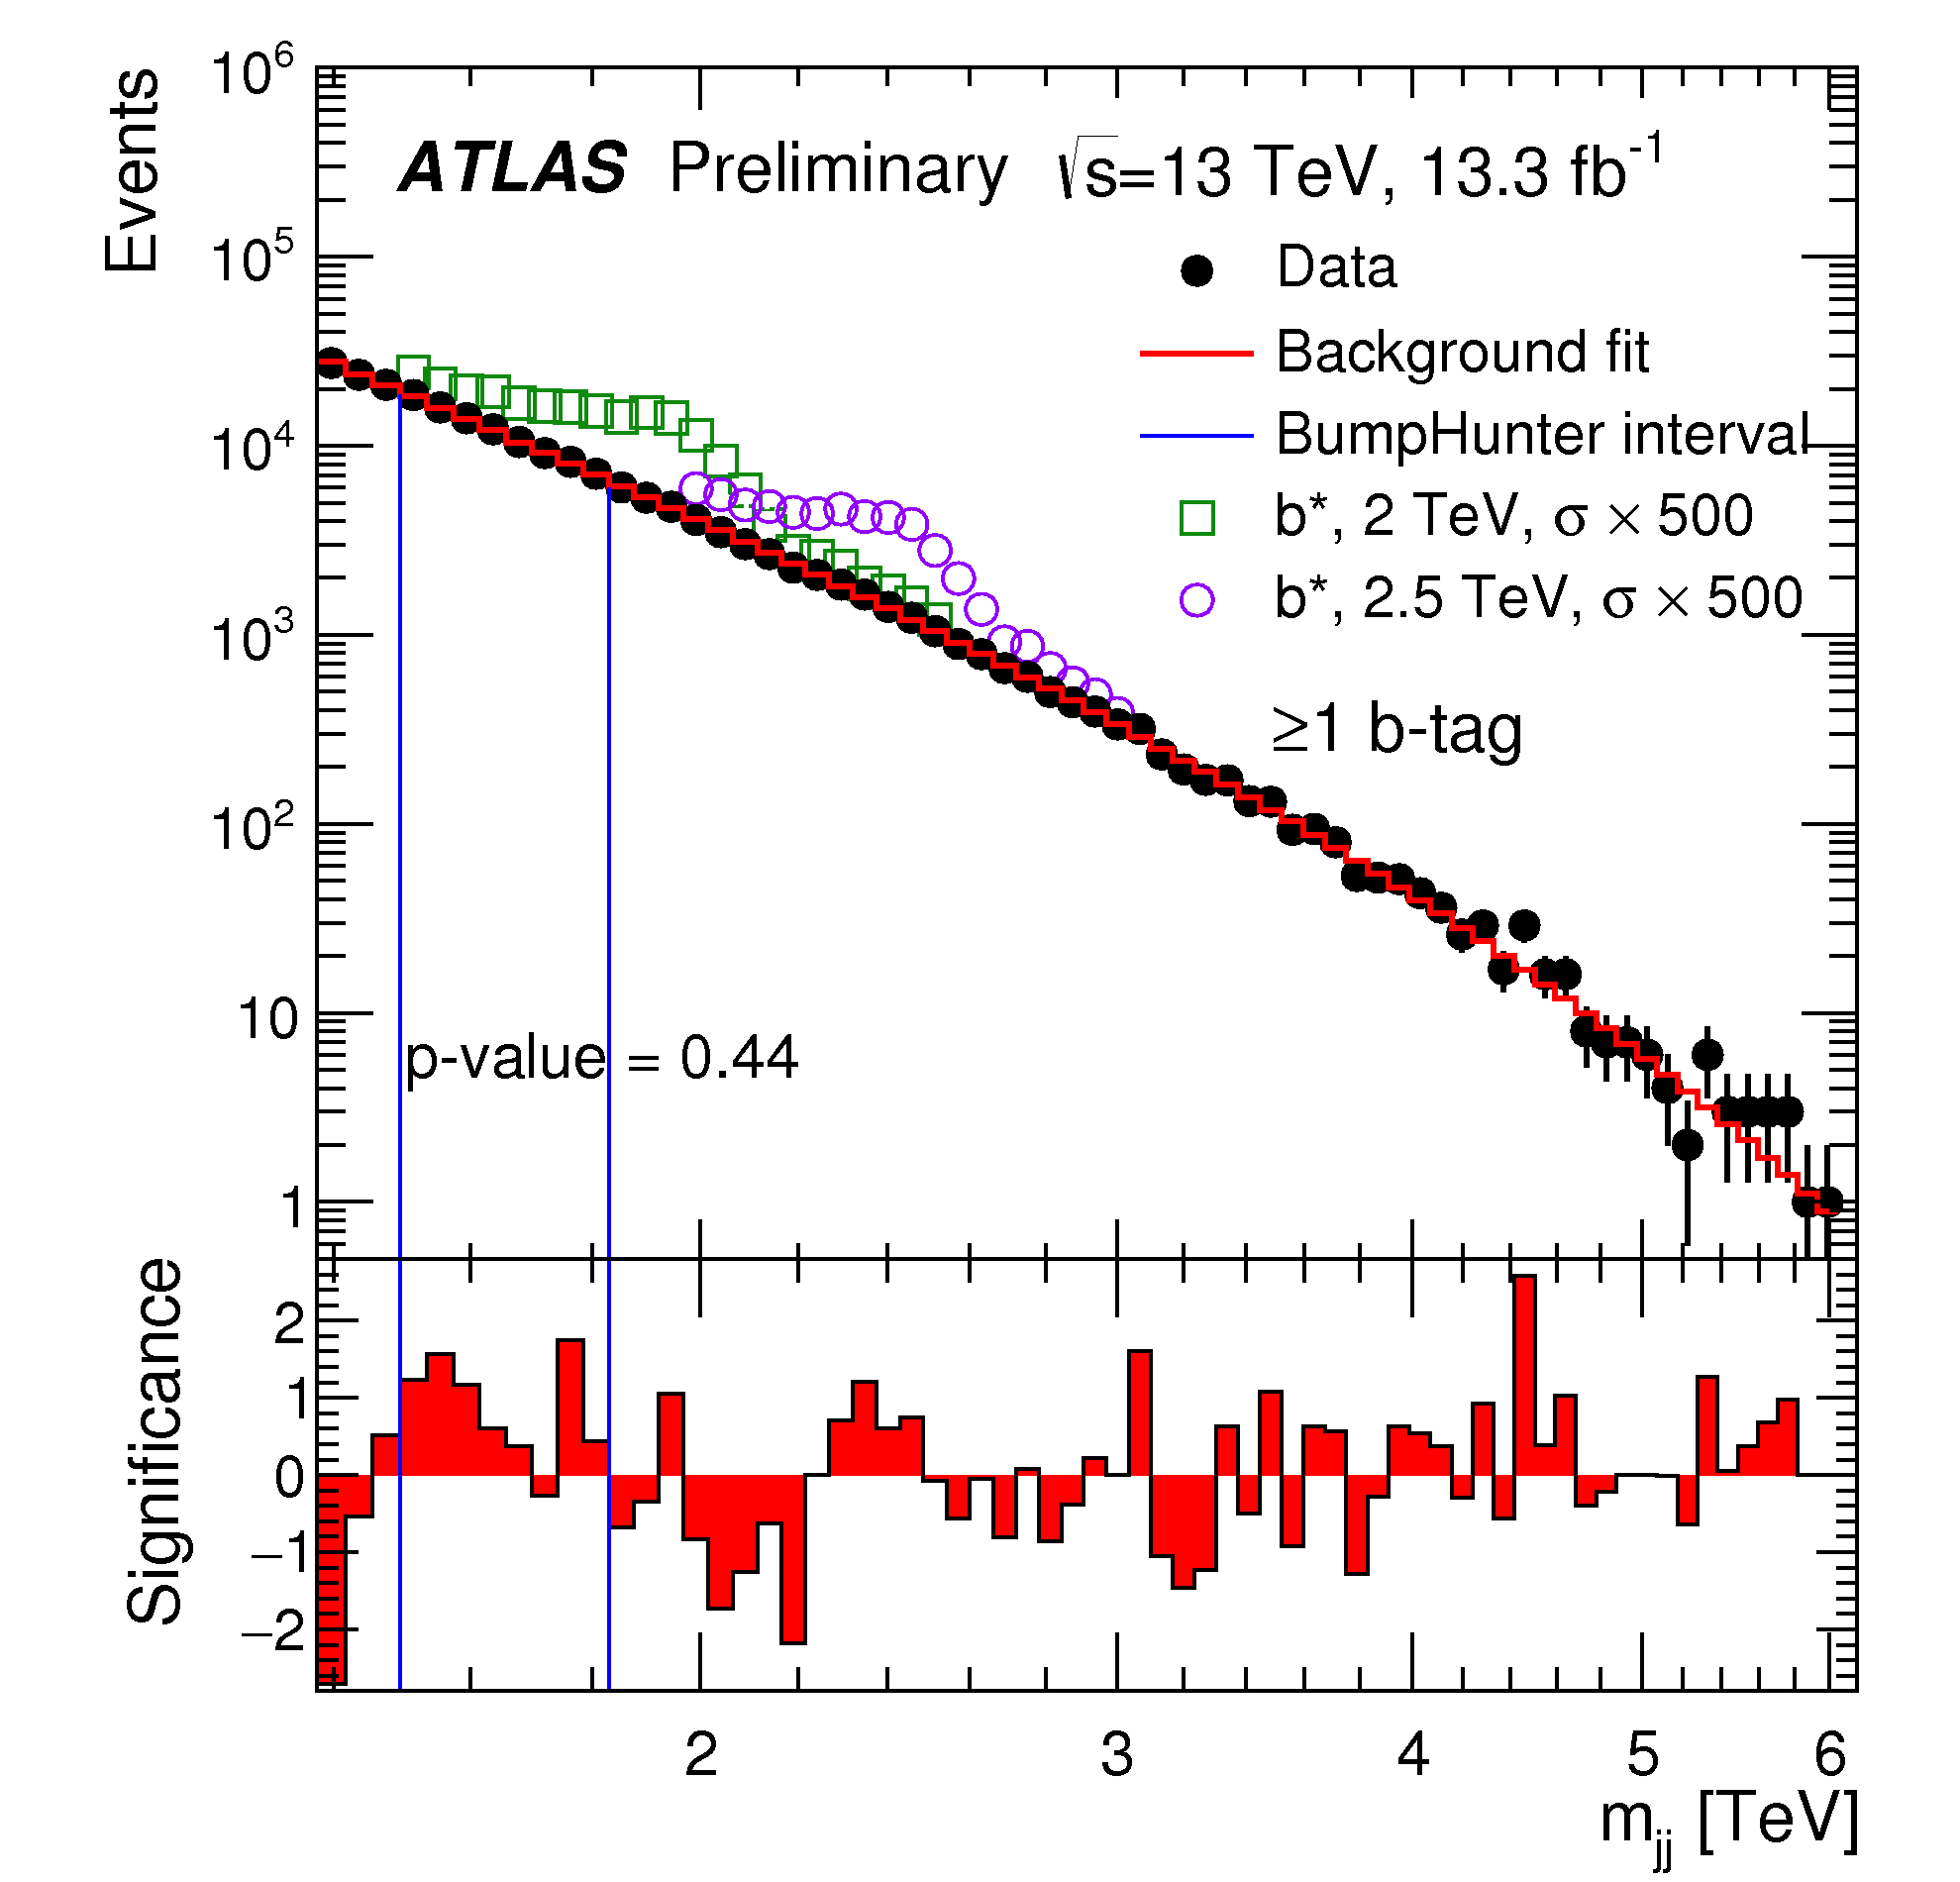
\includegraphics[width=0.65\linewidth, angle=0]{figs/Dibjet/ICHEP/bkg-SearchPhase_b.png}}
  \end{center}
  \caption
      [The dijet mass spectrum of the \summer{} data-set in the 2 and the $\geq$1 $b$-tag category
        compared to the background estimation created using the 3 parameter dijet fit function.
        The most discrepant excess found by the \bh{} algorithm and the associated \mbox{$p$-value} are shown.]        
      {The dijet mass spectrum of the  \summer{} data-set in the (a) 2 and (b) $\geq$1 $b$-tag category
        compared to the background estimation created using the 3 parameter dijet fit function.
        The upper panel shows the data compared to the background estimate,
        benchmark signal models with enhanced cross sections are overlaid.
        The lower panel shows the significance of the difference between the data and the background estimate.
        The most discrepant excess as found by the \bh{} algorithm is indicated by the vertical blue lines and the \mbox{$p$-value} of this excess is printed on the plot~\cite{dibjet-ichep_conf}.
          }
  \label{fig:bkg-summer_searchPhase}
\end{figure}

\clearpage
\section{\lm{} Search Phase}
\label{sec:bkg-full}

This section presents the search phase for the \lm{} data-set:
Section~\ref{sec:bkg-full_fitCR} describes the background-only samples used for the search phase validation studies.
Section~\ref{sec:bkg-full_globalFit} demonstrates that the global fit strategy is not a valid strategy for the \lm{} data-set.
Section~\ref{sec:bkg-full_swift} introduces an alternative background estimation strategy called the Sliding Window Fit (SWiFt)
and Section~\ref{sec:bkg-full_windowSel} describes the strategy used for selecting the parameters of the SWiFt background estimation.
Sections \ref{sec:bkg-full_windowSelTests}~--~\ref{sec:bkg-full_signalInj} show validation studies
of the search phase performed using the SWiFt background estimation.
Sections~\ref{sec:bkg-full_windowSelResults}~--~\ref{sec:bkg-full_results} presents the results of the search phase using the \lm{} data-set.

\subsection{Background-Only Samples}
\label{sec:bkg-full_fitCR}

%The background estimation strategy is tested and developed without using the final data-set, which is known as `blinding'.
%Blinding is required such that no bias from the final data-set is introduced into the background estimation strategy.
%To perform blinded tests a dijet mass spectrum that is representative of the background is required.

To perform the validation studies of the \lm{} search phase
a dijet mass spectrum that represents the shape of the background with no signal contamination is required.
In the \summer{} data-set analysis Monte-Carlo simulation was used,
as described in Section~\ref{sec:bkg-summer_fitCR}.
However, as the \lm{} data-set contains 24.3~\ifb{} of data, Monte-Carlo simulation cannot be produced with a large enough statistical
precision to perform an adequate test of the background estimation strategy.

Instead two background representative data-sets are used:
a 3~\ifb{} subset of data and a high statistical precision fit control region.
The 3~\ifb{} subset of data is created from events drawn at random from the final data spectrum.
Figure~\ref{fig:fittingDataSubset} shows the dijet mass spectrum of the 3~\ifb{} subset and the full \lm{} data-set.
The dijet mass spectrum of the subset represents the shape of the dijet mass spectrum in full data-set,
except with a lower statistical precision.
The luminosity of the subset of data was chosen to be similar to that of a
previous low mass di-$b$-jet search in an equivalent mass range~\cite{dibjet-lhcp_conf},
such that this subset of data is known not to be sensitive to signal.

\begin{figure}[!htb]
\captionsetup[subfigure]{aboveskip=0pt,justification=centering}
\centering
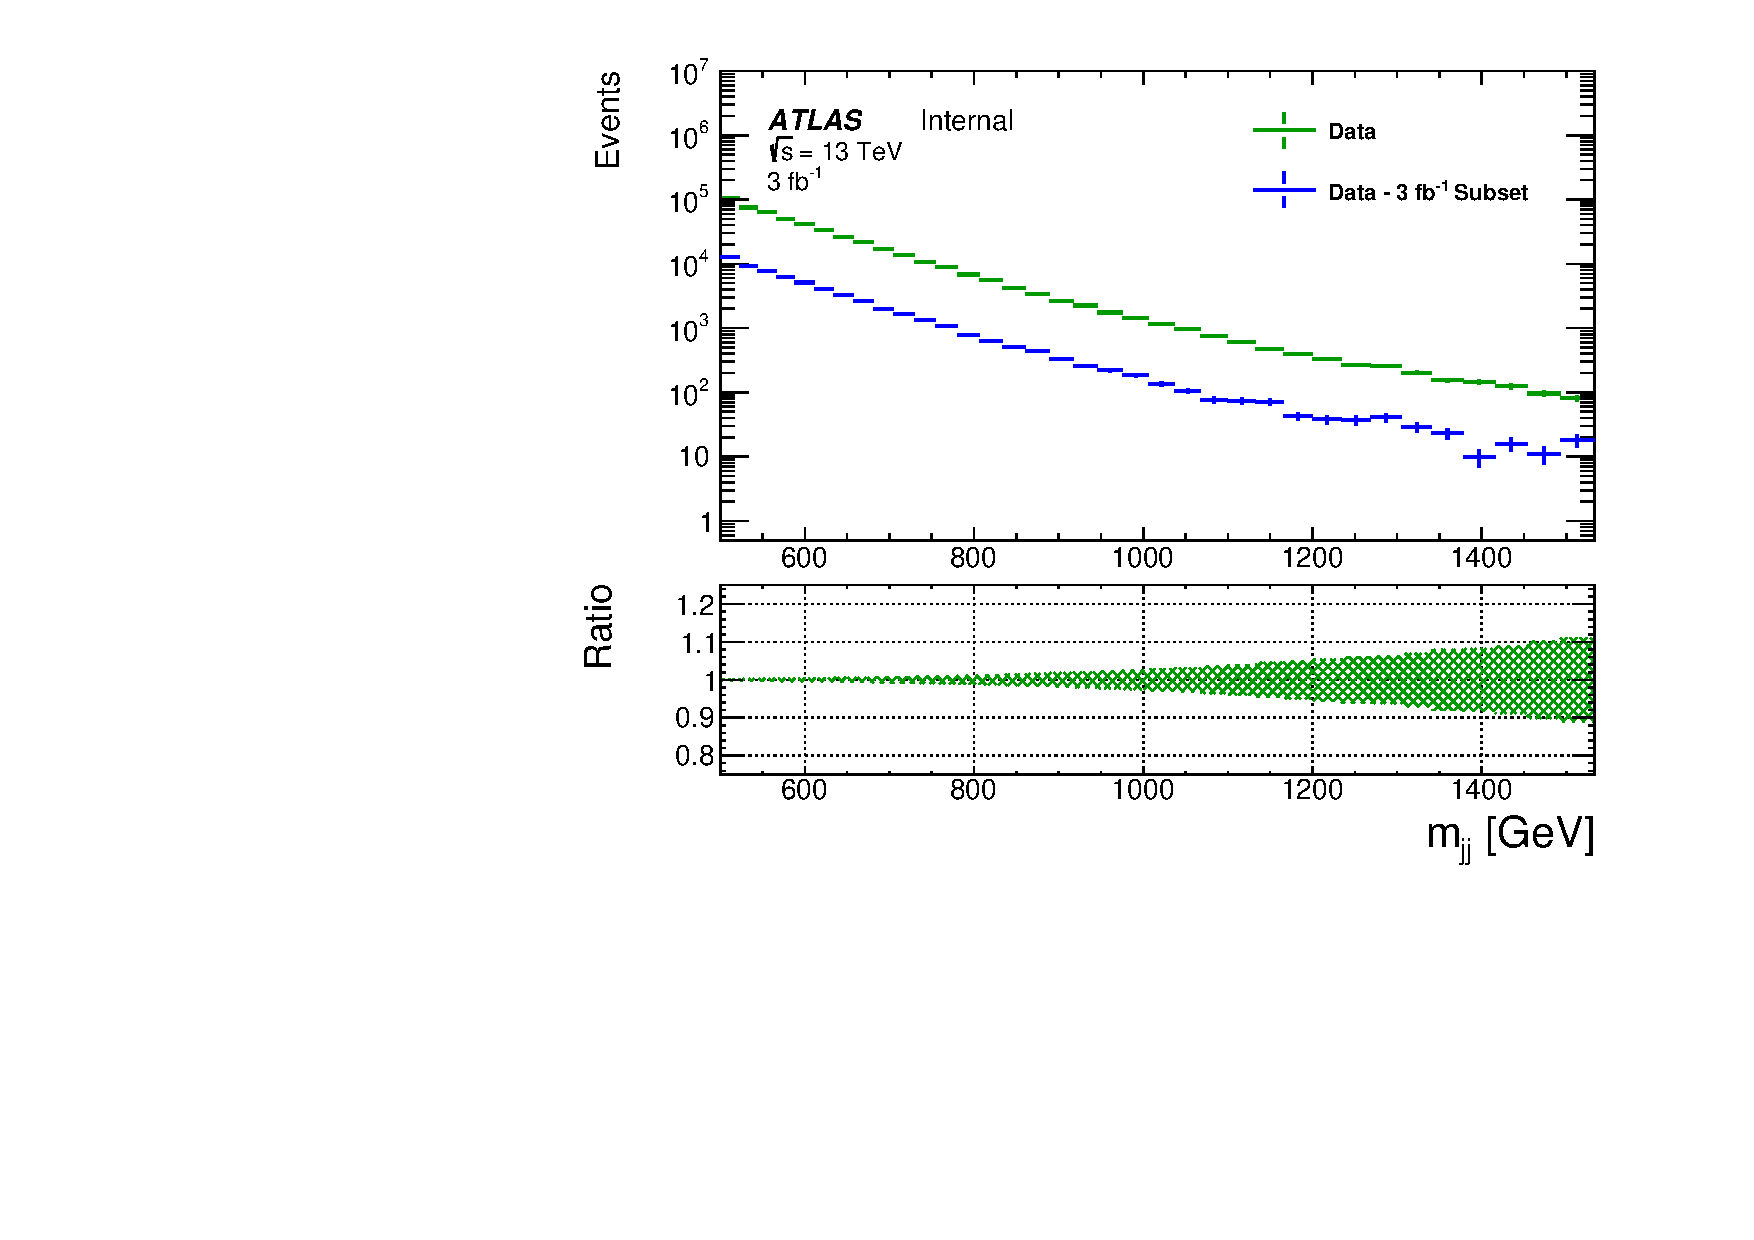
\includegraphics[width=0.7\linewidth, angle=0]{figs/Dibjet/LowMass/FitStudy/subset_dataComp.pdf}
\vspace{-1em}
\caption
    [ The dijet mass spectrum of the full \lm{} data-set and a 3~\ifb{} subset.
      ]
    {\label{fig:fittingDataSubset}
      The dijet mass (\mjj{}) spectrum of the full \lm{} data-set and a 3~\ifb{} subset of \lm{} data.
      The lower panel shows a ratio.}
    \vspace{-1em}
\end{figure}

To create the \lm{} fit control region,
the dijet mass spectrum of events that have passed the
\lm{} event-selection except offline $b$-tagging selection is used,
this is referred to as the 0-tag dijet mass spectrum.
This dijet mass spectrum contains more events than the final dijet mass spectrum
and will have a similar shape as most of the event selection, including online $b$-tagging, has been applied.

To account for the effect of offline $b$-tagging in the fit control region,
the 0-tag data must be multiplied by the event-level offline $b$-tagging efficiency with respect to online $b$-tagging, $\epsilon_b^{\text{offline}}$,
which is defined as the fraction of events that pass offline $b$-tagging requirements given
that the events have passed all other requirements of the \lm{} event selection, including online $b$-tagging.
$\epsilon_b^{\text{offline}}$ is estimated using the ratio
of the dijet mass spectrum from the 0-tag data to the 3~\ifb{} subset of data;
Figure~\ref{fig:fittingCR}(a) shows the two dijet mass spectra and the ratio.
The ratio is then scaled by 24.3/3 to account for the lower luminosity of the subset of data,
and is smoothed using the five parameter dijet fit function.
Figure~\ref{fig:fittingCR}(b) shows the luminosity adjusted ratio (black points) and the fit (red line).
The goodness of fit is estimated by comparing the $\chi^2$ test statistic to a $\chi^2$ distribution with the same number of degrees of freedom;
a $\chi^2$ $p$-value of 0.053 is observed indicating a reasonable fit quality.

The 0-tag spectrum is then scaled by the smoothed estimation of $\epsilon_b^{\text{offline}}$ to create the dijet mass spectrum of the fit control region.
Figure~\ref{fig:fittingCR}(c) shows the dijet mass spectrum from the full \lm{} data-set and the fit control region,
showing that the fit control region gives a reasonable background-only sample for search phase validation studies.

Two types of dijet mass spectra are created using the fit control region for the search phase validation studies.
The first is a \textit{`smooth'} dijet mass spectrum, where the uncertainties on the fit control region are set to be Poisson like,
which means that the uncertainty is the square root of the number of events.
This is done such that the uncertainties represent the size of statistical fluctuations expected in the full \lm{} data-set.
The second type of dijet mass spectrum is a \textit{`data-like'} dijet mass spectrum,
where a random set of Poisson fluctuations are applied to the fit control region,
to represent the statistical fluctuations that are observed in data.
Many data-like dijet mass spectra can be made, each representing a different set of random fluctuations.
Figure~\ref{fig:fittingCR}(d) shows the comparison of the smooth spectrum and a data-like spectrum.

\begin{figure}[!htb]
\captionsetup[subfigure]{aboveskip=0pt,justification=centering}
\centering
\hspace{-2mm}
\subcaptionbox{} {
  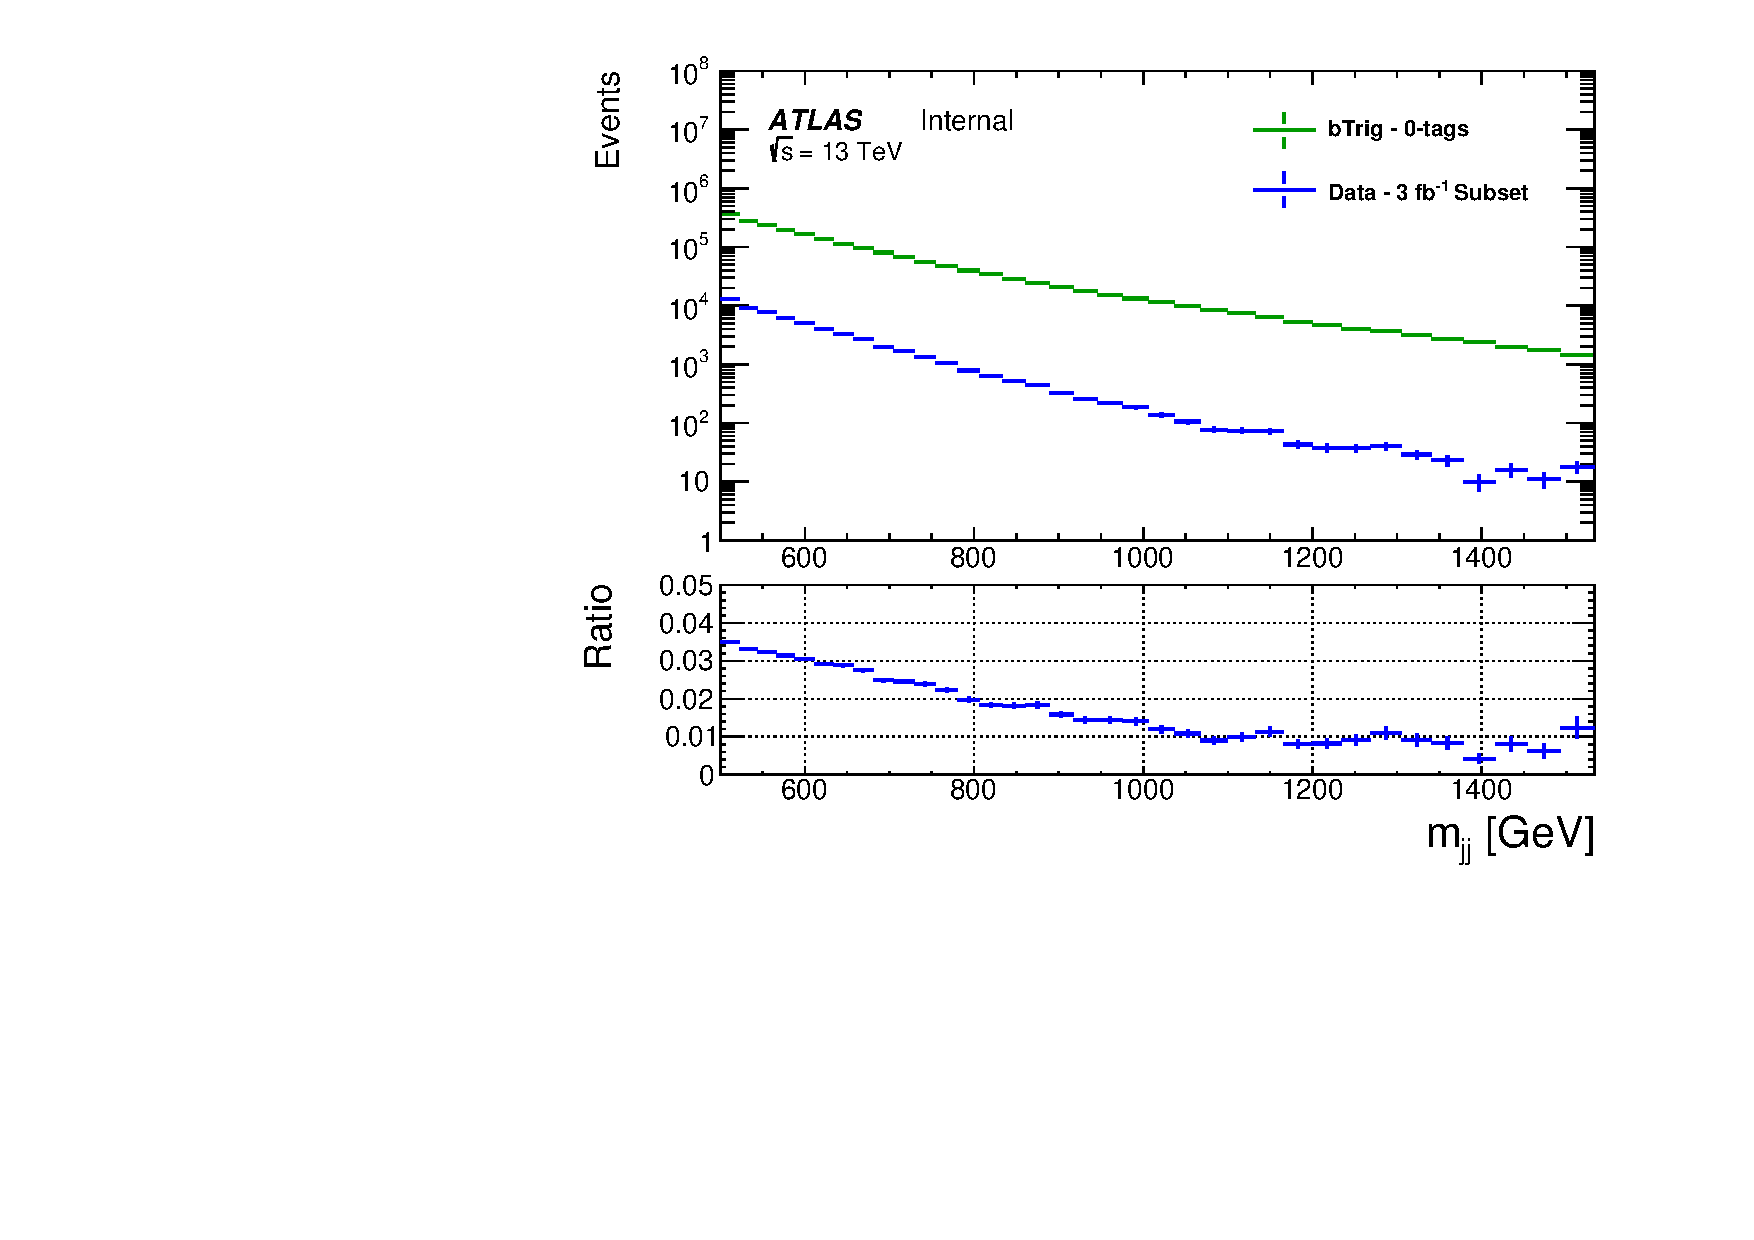
\includegraphics[width=0.51\linewidth, angle=0]{figs/Dibjet/LowMass/FitStudy/corrFitCR_0tag_subset.pdf}\vspace{-1mm}
}\hspace{-8mm}
\subcaptionbox{} {
  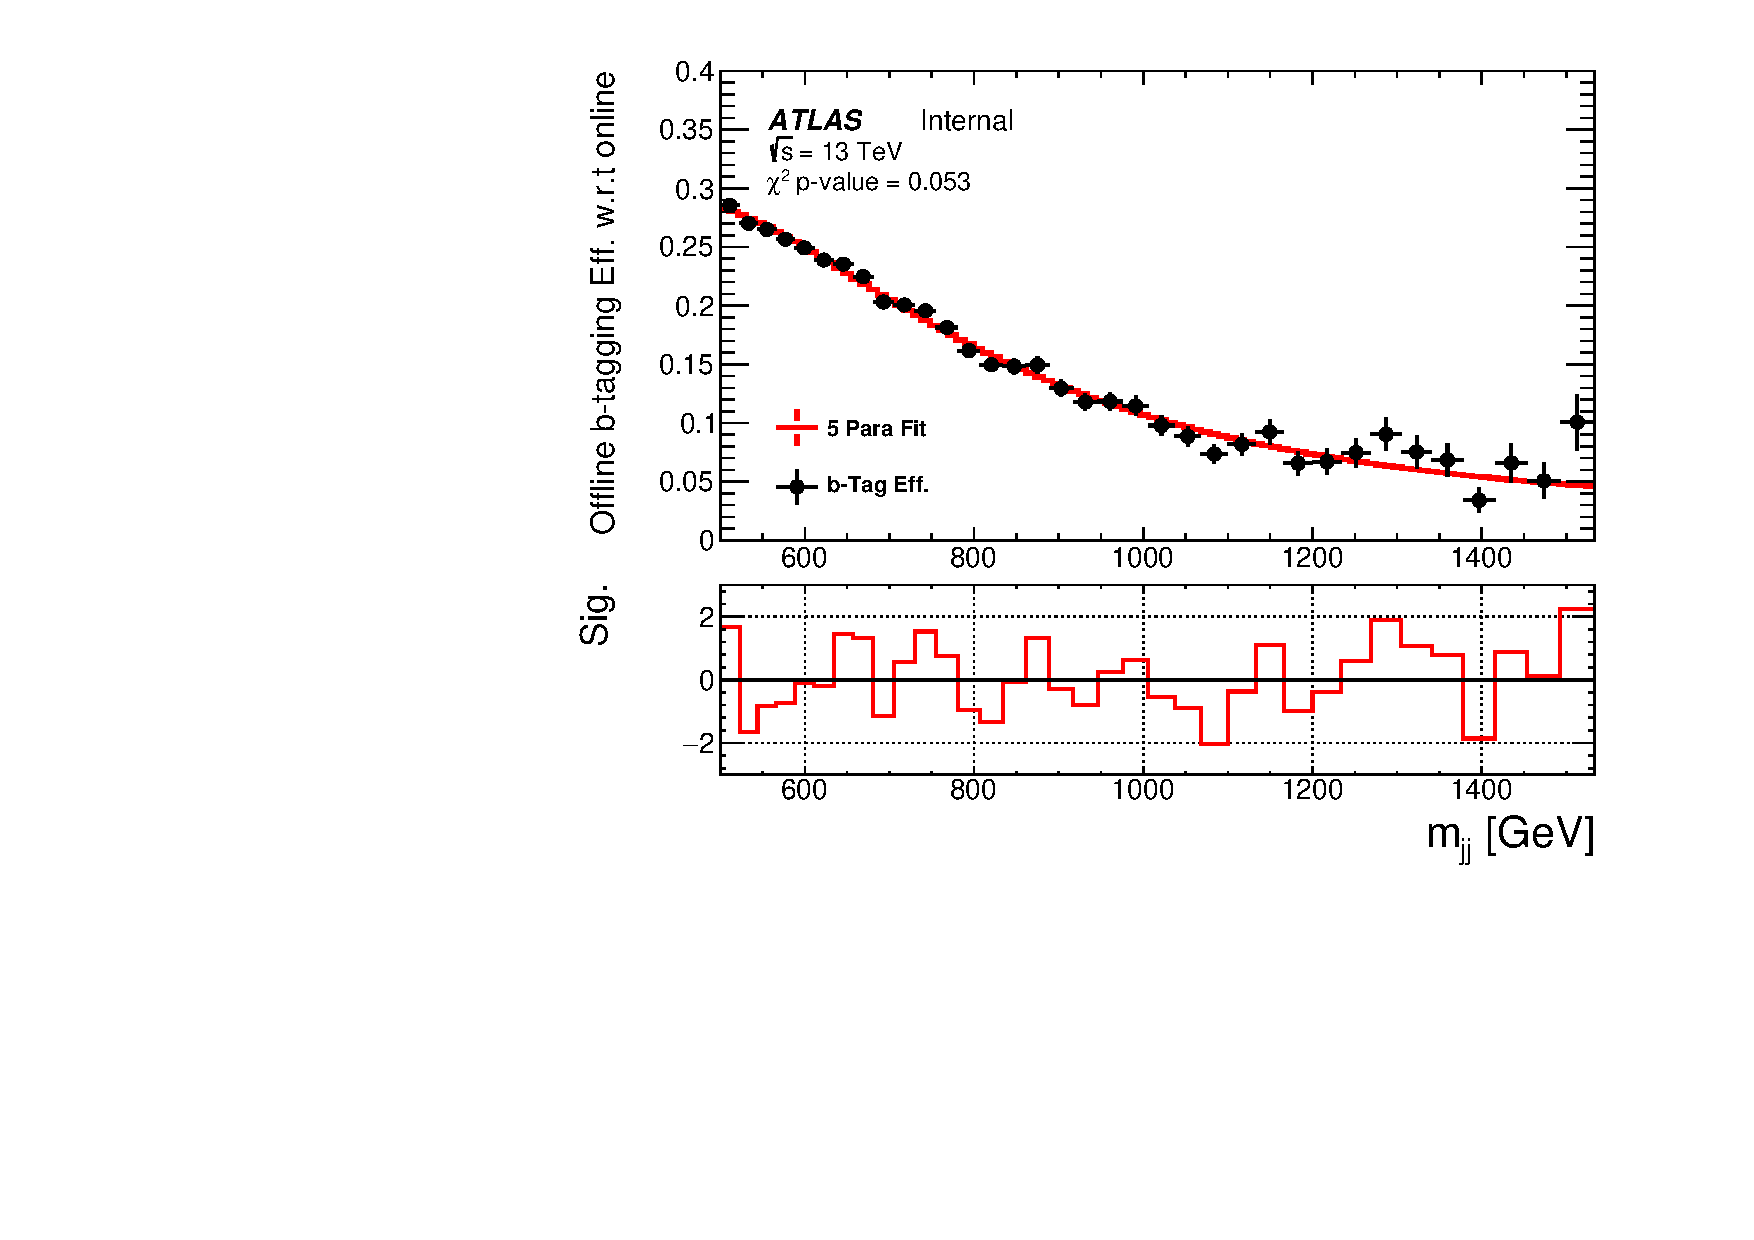
\includegraphics[width=0.51\linewidth, angle=0]{figs/Dibjet/LowMass/FitStudy/corrFitCR_5parFit.pdf}\vspace{-1mm}
} \hspace{-2mm} \vspace{1.5em}
\hspace{-2mm}
\subcaptionbox{} {
  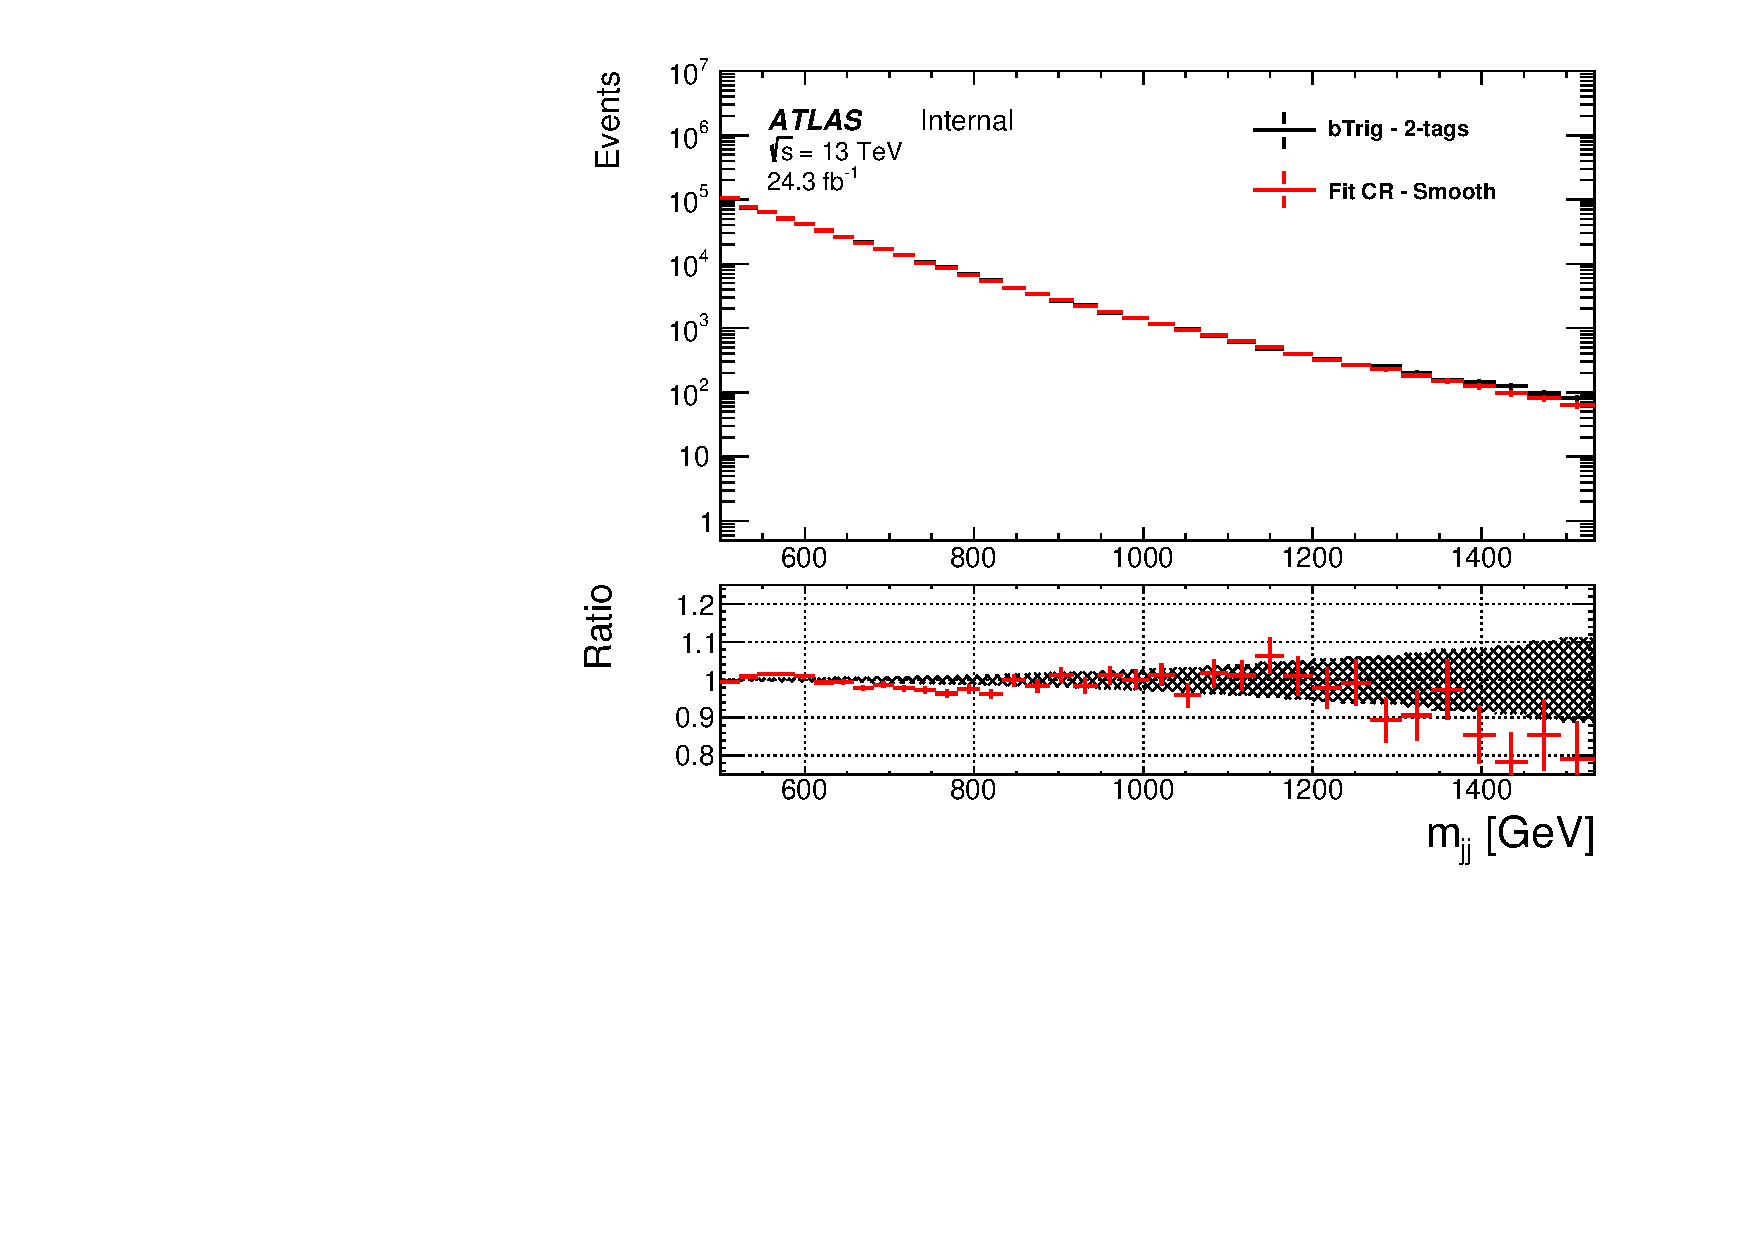
\includegraphics[width=0.51\linewidth, angle=0]{figs/Dibjet/LowMass/FitStudy/corrFitCR_dataComp.pdf}\vspace{-1mm}
}\hspace{-8mm}
\subcaptionbox{} { 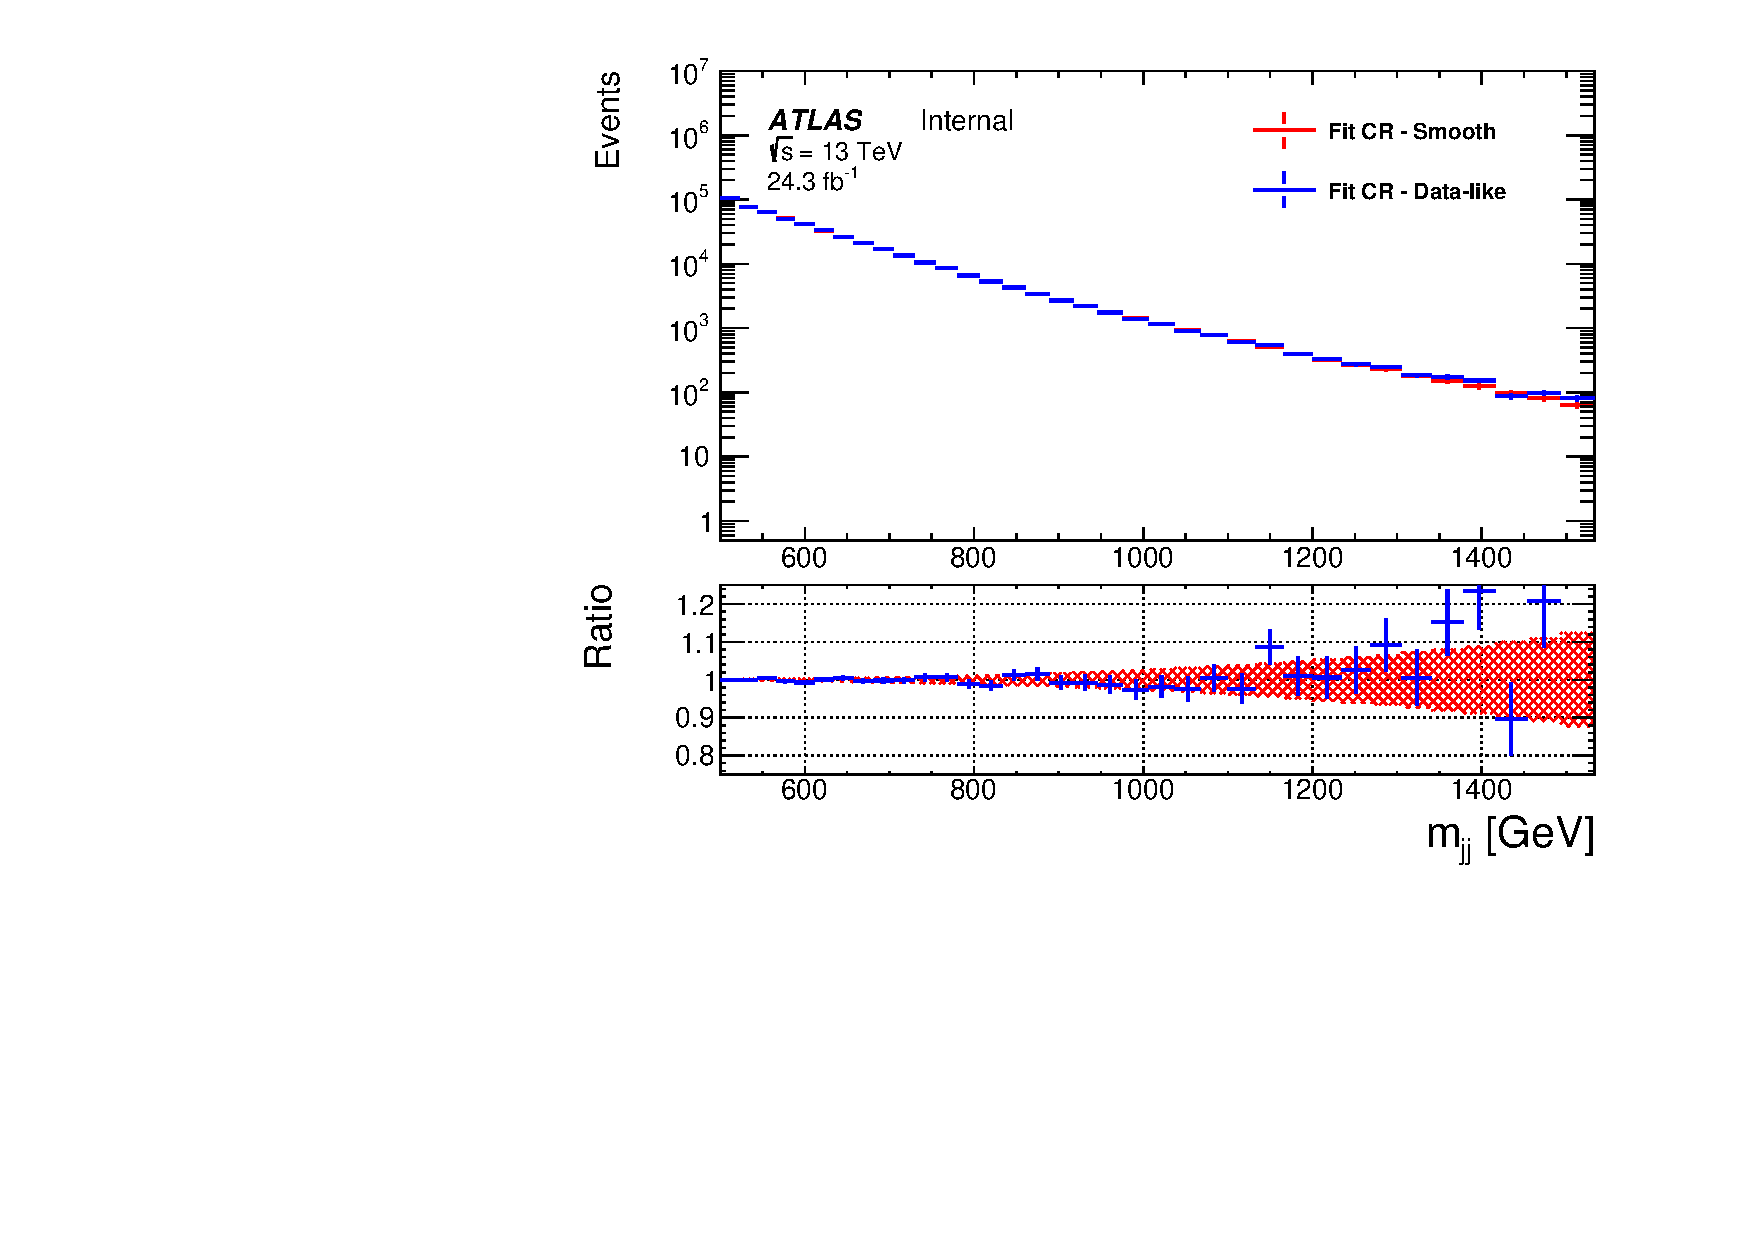
\includegraphics[width=0.51\linewidth, angle=0]{figs/Dibjet/LowMass/FitStudy/corrFitCR_smooth_dataLike.pdf}\vspace{-1mm}
}
\hspace{-2mm}
\vspace{-1em}
\caption
    [A figure showing the process of obtaining the fit control region dijet mass spectrum
      used for the \lm{} data-set fit studies.
    ]
    {\label{fig:fittingCR}
      A figure showing the process of obtaining the fit control region dijet mass ($m_{jj}$) spectrum
      used for the \lm{} data-set fit studies.
      Panel (a) shows the dijet mass spectrum of events before $b$-tagging is applied (0-tag) and of a 3~\ifb{} subset of \lm{} data.
      Panel (b) shows the offline $b$-tagging efficiency with respect to online $b$-tagging estimated using the luminosity adjusted ratio of the two spectra in plot (a),
      the lower panel shows the significance of difference between the luminosity adjusted ratio and the fit.
      Panel (c) shows the dijet mass spectrum of the fit control region and the full \lm{} data-set.
      Panel (d) shows the smooth and data-like dijet mass spectra from the fit control region.
}
\end{figure}

%The 0-tag data will be insensitive to signal as no offline $b$-tagging is applied, hence will have larger light and charm jet impurities
As no offline $b$-tagging is applied,
the 0-tag data contains larger light jet and $c$-jet impurities than the full \lm{} data-set
and hence is considered insensitive to signal.
As has been discussed above, the  3~\ifb{} subset of data will not be sensitive to signal.
Therefore the fit control region is insensitive to signal and can be considered a background-only spectrum.

All search phase validation studies for the \lm{} data-set are performed in the mass region outlined by the \lm{} event selection, 566-1533~GeV.
However, the fit control region is created in the dijet mass region 500-1533 GeV
because the fit control region was created before the bias due to non-leading jets, described in Section~\ref{sec:evt-sel_btrigMatch}, was observed.
As the fit control region is created by applying a smoothed efficiency to each independent dijet mass bin,
the bias will not affect events with \mjj{} $>$ 566 GeV.

The use of the subset of data and the fit control region gives two complementary dijet mass spectra to perform search phase validation studies.
The subset is representative of the same underlying dijet mass spectrum as the full \lm{} data-set but has lower precision.
The fit control region, provides a high-statistic background-only spectra with a similar shape to the dijet mass spectrum of the full \lm{} data-set.

%However, as shown above, it does not have an identical shape to the final distribution, hence we also want to consider another test data set with an identical shape. 
%% Add this line if describing subset of data.


%\subsubsection{High Mass}
%\label{sec:bkg-full_highmass_bkgsample}

\subsection{Global Fit Strategy}
\label{sec:bkg-full_globalFit}

Using a single dijet fit function to model the full mass range considered is known as the global fit strategy.
Previous di-$b$-jet searches have used a global fit strategy~\cite{dibjet-mori16_paper}, including the \summer{} analysis described above.
%Hence, the global fit strategy is the first strategy that is tested for the \lm{} data-set.

%\subsubsection{Low Mass}
%\label{sec:bkg-full_lowmass_globalFit}

Figure~\ref{fig:lowmass_globalFit} shows the smooth dijet mass spectrum from the fit control region
fitted to using the global fit strategy with the 3, 4 and 5 parameter dijet fit functions.
The lower panel shows the significance of the difference between the data and the various fits.
One would expect an excellent fit quality when an appropriate background estimation is used
to model the smooth spectrum as the uncertainties are larger than the true statistical fluctuations present.
The 3 parameter dijet fit function has a $\chi^{2}/\text{n.d.f.} = 3.65$,
where $n.d.f.$ represents the number of degrees of freedom, demonstrating an extremely poor fit quality;
hence, the 3 parameter dijet fit function is rejected.
Further to this, there is a fit bias present for all dijet fit functions,
where a fit bias is defined as a difference between the background estimation and the true underlying dijet mass spectrum of the background.
The bias is observed as a set of peaks and troughs in the significance plot.
A fit bias that is similar in size to the statistical fluctuations
may cause a peak to be falsely interpreted as signal or for a trough to mask true signal.

To further quantify the effect of the fit biases in the 4 and 5 parameter case,
Figure~\ref{fig:bhFit_lm_global} shows the two global fits after the \bh{} algorithm has been performed.
The \bh{} algorithm assigns \mbox{$p$-values} of 0.418 and 0.513 to the largest excesses in the 4 parameter and 5 parameter case respectively.
In the case of the smooth dijet mass spectrum, the \bh{} \mbox{$p$-value} cannot be interpreted in the conventional way,
as the smooth spectrum does not contain the Poisson fluctuations that are present in the pseudo-experiments it is being compared to.
Instead, it provides an approximate estimation of the size of the largest fit bias to the size of the largest excesses expected in data due to statistical fluctuations.
The fit biases in the global fit for the 4 and 5 parameter dijet fit functions are large relative to the size of statistical fluctuations expected.
It is therefore concluded that neither fit function provides an adequate description of the background.

\newpage
As a result, the global fit strategy is rejected and an alternative background modelling strategy is used.
It is not unexpected that the global fit strategy is inadequate for large luminosities and wide mass ranges,
as the resulting small statistical uncertainties and large fit ranges mean that any
difference between the underlying shape of the QCD dijet mass spectrum
and the dijet fit functions are significant.

\begin{figure}[!htb]
\centering
\includegraphics[width=0.6\linewidth, angle=0]{figs/Dibjet/LowMass/FitStudy_min566/globalFit_lm_dh.pdf}
\caption
    [ The smooth dijet mass spectrum from the \lm{} fit control region
      fitted to using the 3, 4 and 5 parameter global fits.
    ]
    {\label{fig:lowmass_globalFit}
      The smooth dijet mass spectrum from the \lm{} fit control region
      fitted to using the 3, 4 and 5 parameter global fits.
      The lower panel shows the significance of the difference between the data and the background fits.}
\end{figure}
\begin{figure}[!htb]

\captionsetup[subfigure]{aboveskip=0pt,justification=centering}
\centering
\subcaptionbox{4 parameters, Global} {
  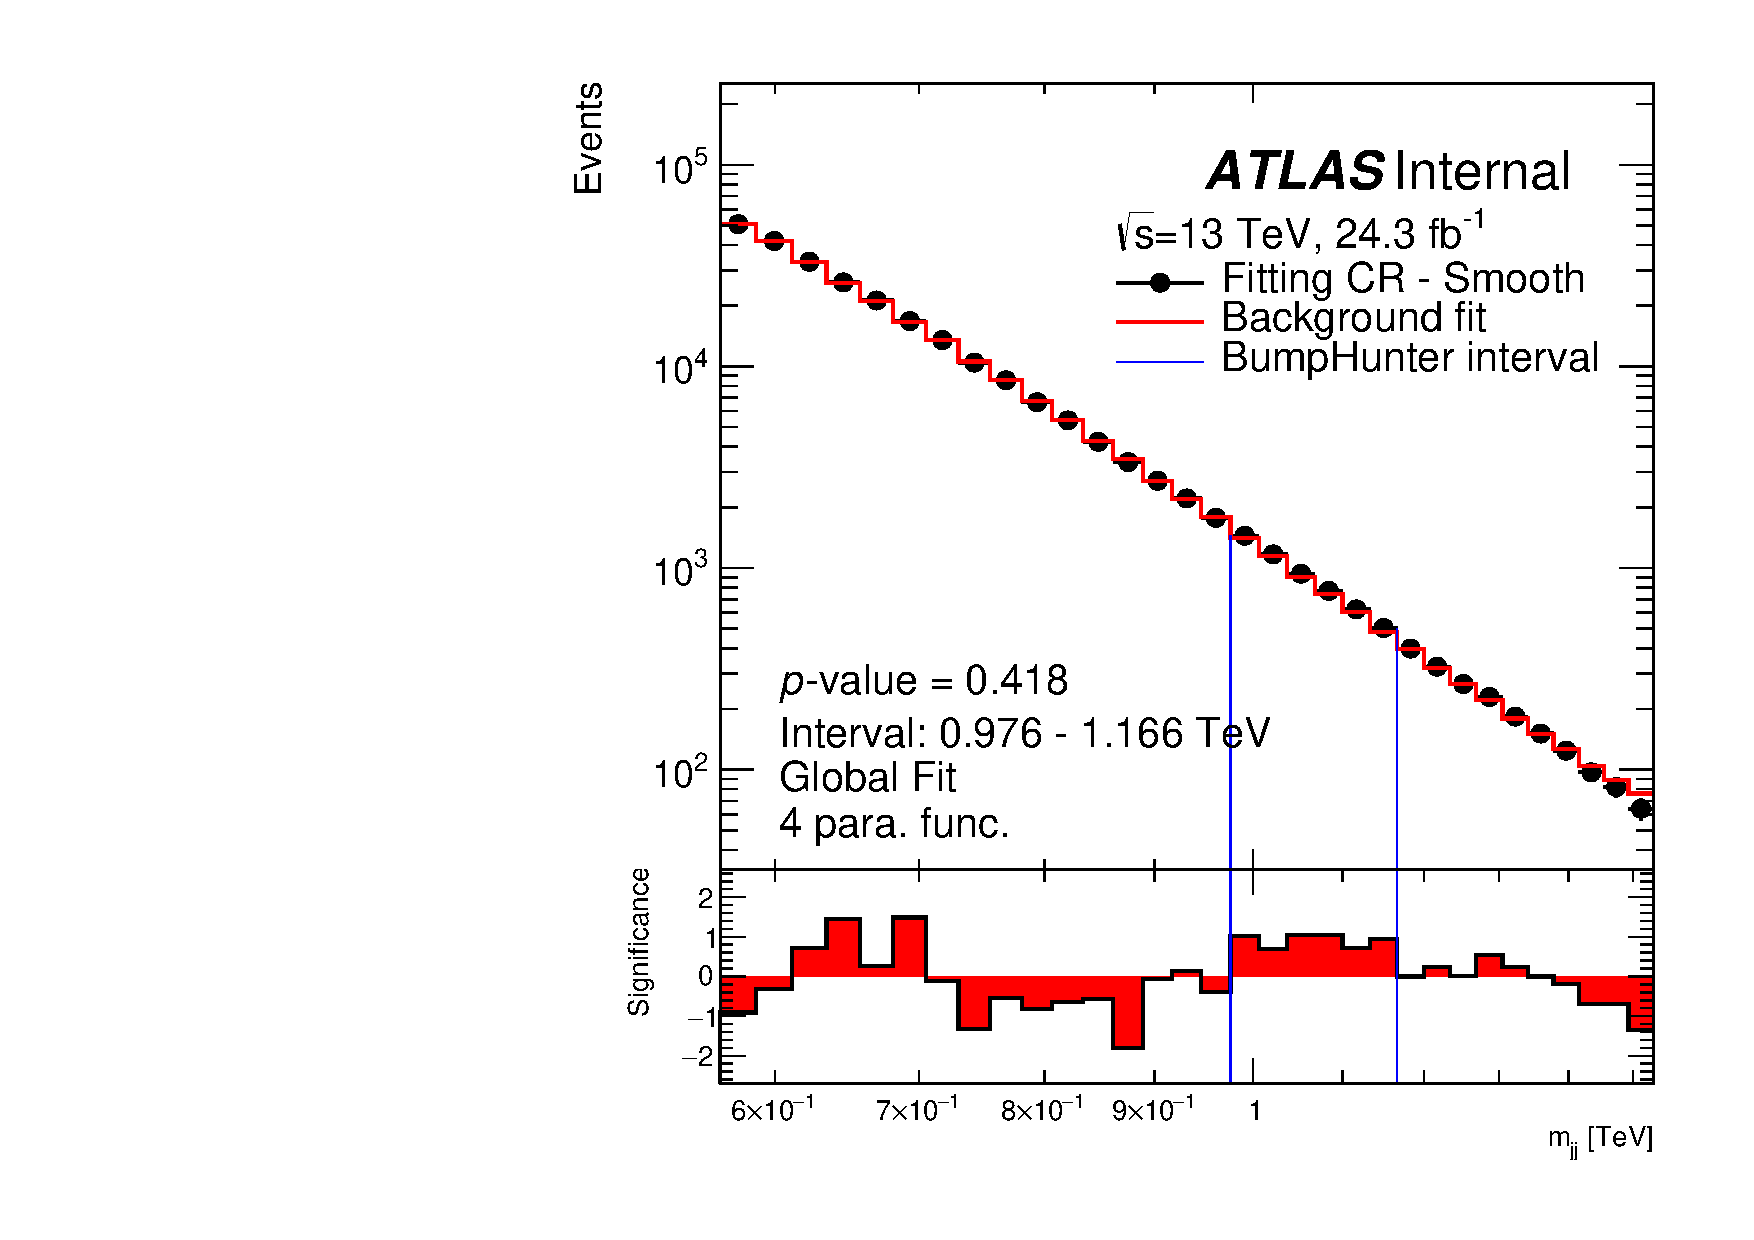
\includegraphics[width=0.45\linewidth, angle=0]{figs/Dibjet/LowMass/FitStudy_min566/globalFit_lm_bH_4para.pdf}
}
\subcaptionbox{5 parameters, Global} {
  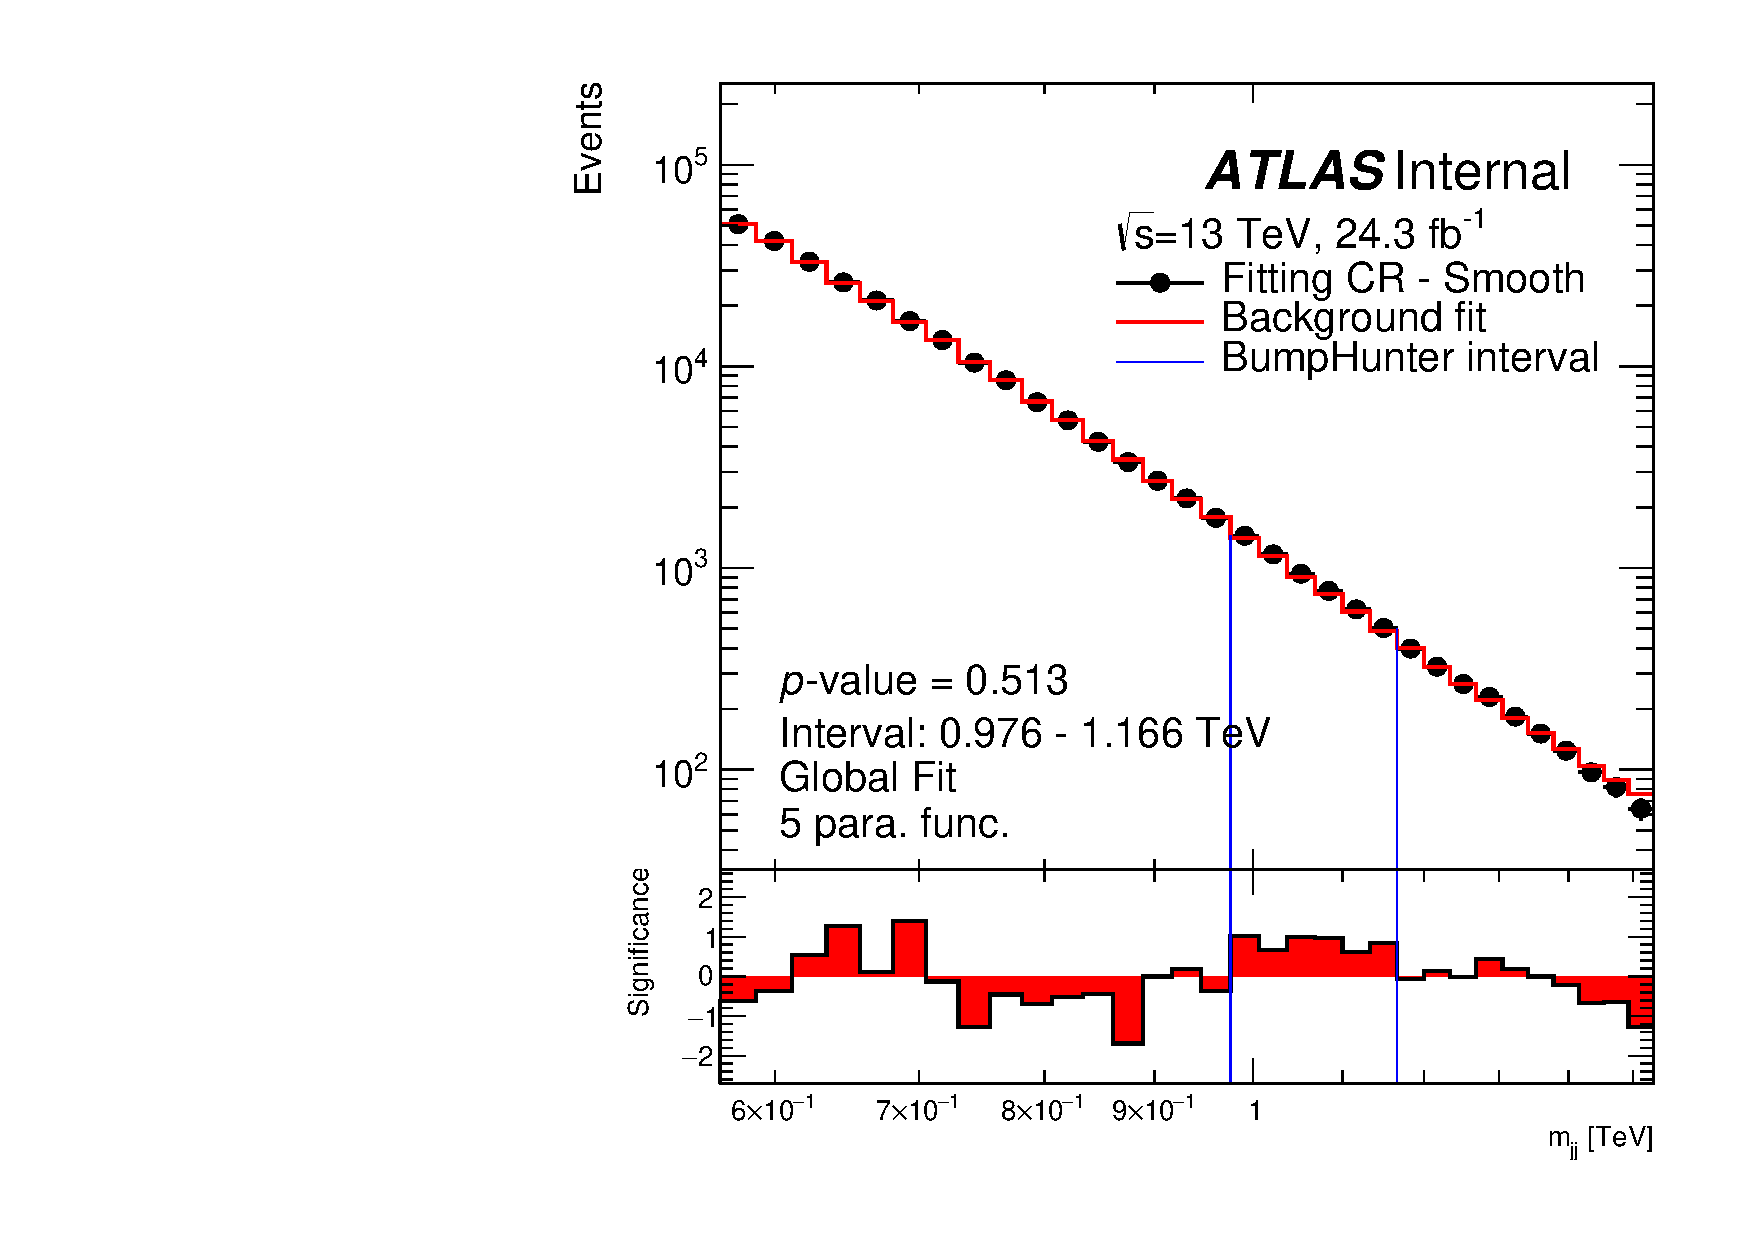
\includegraphics[width=0.45\linewidth, angle=0]{figs/Dibjet/LowMass/FitStudy_min566/globalFit_lm_bH_5para.pdf}
}
\caption
    [The global fit performed on the smooth dijet mass spectrum from the \lm{} fit control region
      using the 4 and 5 parameter dijet fit functions.
    ]
    {\label{fig:bhFit_lm_global}
      The global fit and \bh{} algorithm procedure run on the smooth dijet mass spectrum from the \lm{} fit control region
      using the 4 and 5 parameter dijet fit functions.
      The upper panel shows the data compared to the background estimate and the lower panel shows the significance of the difference between the two.
      The most discrepant excess as found by the \bh{} algorithm is indicated by the vertical blue lines and the \mbox{$p$-value} of this excess is printed on the plot. }
\end{figure}


%\subsubsection{High Mass}
%\label{sec:bkg-full_highmass_globalFit}

\newpage
\subsection{Sliding Window Fit Background Estimation (SWiFt)}\label{sec:bkg-full_swift}

As the global fit strategy cannot provide a valid background estimation in the
\lm{} fit control region, an alternate background modelling strategy must be used.

The Sliding Window Fit (SWiFt) background estimation divides the dijet mass spectrum into many overlapping windows,
and performs a local fit in each window to provide one point in the dijet mass background estimate.
This makes the SWiFt method more stable than the global fit at higher luminosities as the mass range of each fit is reduced.
The SWiFt background estimation has been used in the inclusive dijet analysis on the full 2015+2016 ATLAS data-set~\cite{dijet-mori17_paper}.

The windows used by the SWiFt background estimate are centred at each of the
bin boundaries defined by the dijet mass bins, which are shown in Appendix~\ref{app:dijet_bins}.
The window width is defined by fixing the number of bins below the window centre ($n_{\text{Low}}$)
and fixing the number of bins above the window centre ($n_{\text{High}}$).
For this analysis symmetric windows are used, defined by their window half-width ($wHW$); i.e. $n_{\text{Low}}$ = $n_{\text{High}}$ = $wHW$.
Windows are required to have a lower mass bound that is $\geq566$~GeV, which is the dijet mass requirement of the event-selection.
Figure~\ref{fig:bkg-lm_swiftBins} shows the SWiFt windows used in the \lm{} data-set analysis for the window half-widths of 10, 12, 14 and 16.
%The procedure for choosing the window half-width is described in Section~\ref{sec:bkg-full_windowSel}

\vspace{-1em}
\begin{figure}[!htb]
\centering
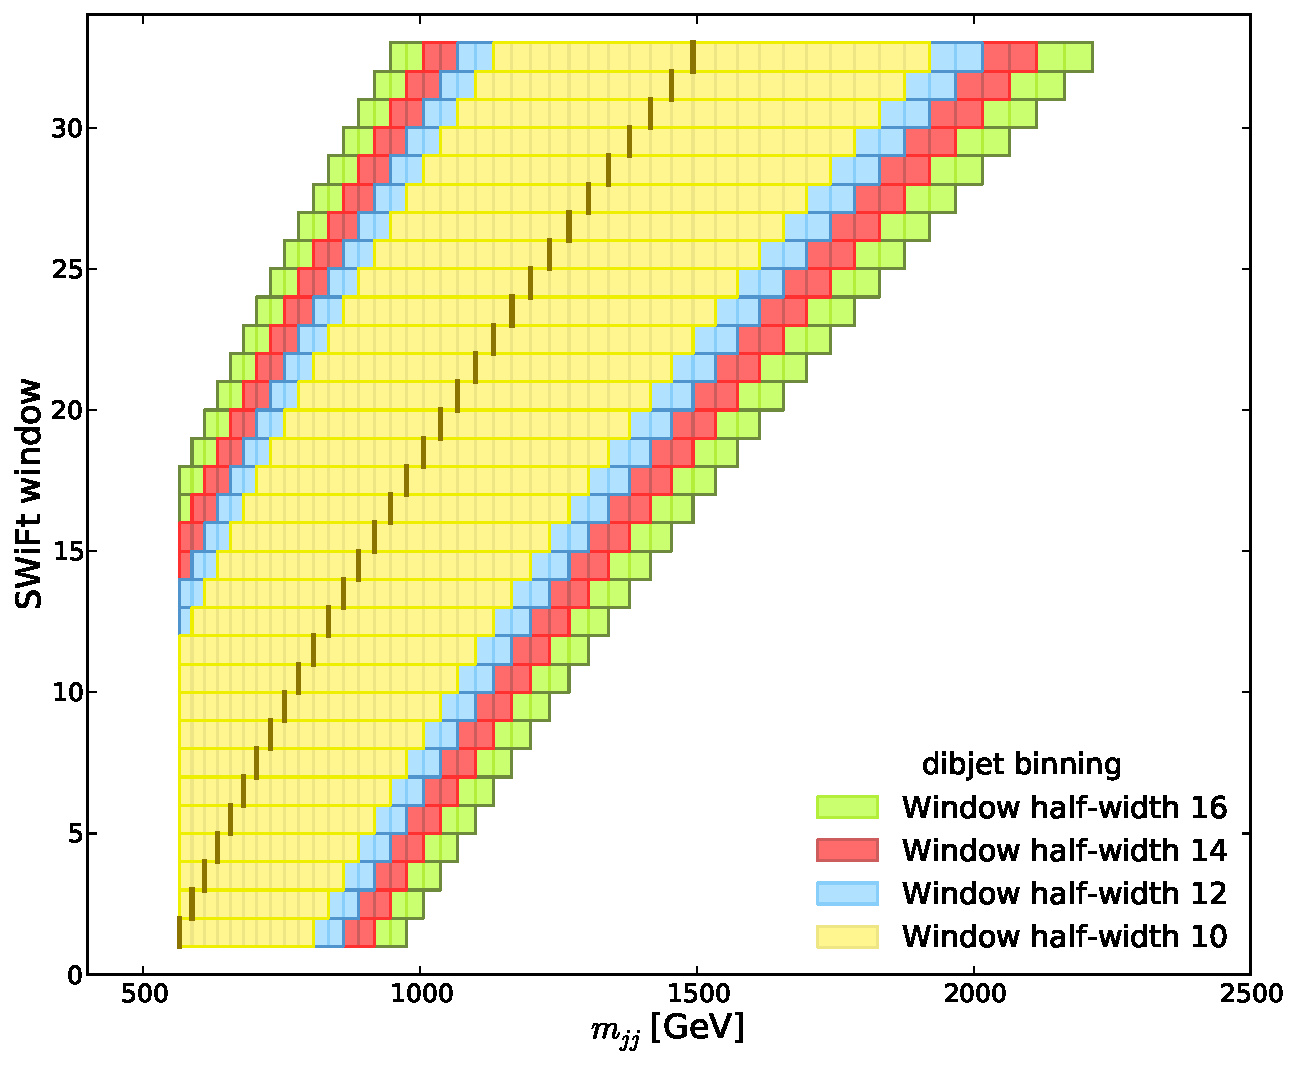
\includegraphics[width=0.75\linewidth, angle=0]{figs/Dibjet/LowMass/evt-swiftBins_min566_fl0_fh0_tr0.pdf}
\vspace{-0.5em}
\caption[The windows used by the SWiFt background estimate in the \lm{} data-set analysis for a range of window half-widths.]
        {\label{fig:bkg-lm_swiftBins}
  The windows used by the SWiFt background estimate in the \lm{} data-set analysis for a range of window half-widths.
  The bin centre is indicated by the black mark and the corresponding window is indicated by the coloured squares.}
\end{figure}

Windows symmetric in the number of dijet mass bins either side of the centre are chosen
as this ensures that there will be an adequate side band on either side of the window centre where possible
and reduces the number of parameters that have to be tested.
For clarity, it should be noted that because the width of the dijet mass bins is not uniform, the windows used are not exactly symmetric with respect to dijet mass;
this effect can be seen in Figure~\ref{fig:bkg-lm_swiftBins}.
Furthermore, it must be noted that enforcing the requirement that the lower mass bound is $\geq566$~\GeV{}
means that for the lowest mass windows $n_{\text{Low}} < n_{\text{High}}$;
again this effect can be clearly seen in Figure~\ref{fig:bkg-lm_swiftBins}.

In each window a fit to the data is performed using one of the dijet fit functions listed in Table~\ref{tab:bkg-fit}.
The same function is used in all windows, with parameters initially seeded from a configuration file and then from the previous fit.
Each of the fits are evaluated at the dijet mass bin which is at the centre of the window, the value is the background estimation for that bin.
The SWiFt background estimation for the full dijet mass spectrum is constructed by combining the single bin background estimations from each of the window fits.

Once, a SWiFt background estimation is constructed,
it is then compared to data using the \bh{} algorithm which finds the most discrepant excess region and assigns a \mbox{$p$-value} to it.
The combination of the SWiFt background estimation and \bh{} algorithm is referred to as the SWiFt search phase.
In the following SWiFt validation studies 1,000 pseudo-experiments are used to calculate the \bh{} \mbox{$p$-value}.

\subsection{Window Selection Strategy}
\label{sec:bkg-full_windowSel}

%As described above, the SWiFt background estimation involves breaking the spectrum up into smaller windows and performing a fit in each window.
%Hence, there are two key input parameters of the SWiFt background estimation:
There are two key input parameters of the SWiFt background estimation:
\begin{enumerate}[leftmargin=*]
\item \textbf{The window width:}\\
  In this analysis symmetric windows are used, therefore the width of the windows is defined by the window half-width ($wHW$) parameter.\vspace{0.5em}
\item \textbf{Fit function:}\\
  The dijet fit functions are used, as used in the global fit strategy. \\
  The functions are listed in Table~\ref{tab:bkg-fit}.
\end{enumerate}
The chosen window half-width and fit function is referred to as the SWiFt configuration.
The best sensitivity to signal is achieved by using the largest window width and the dijet fit function with the fewest number of parameters, whilst still obtaining sufficient fit quality.
Sensitivity studies that demonstrate this statement are shown below in Section~\ref{sec:bkg-full_signalInj}.

\newpage
\noindent
To define `sufficient fit quality' the following fit quality criteria is used:
\begin{itemize}[leftmargin=*]  
\item \textbf{Global $\chi^{2}$ \mbox{$p$-value} $>$ 0.05}:\\
  The $\chi^{2}$ test statistic is calculated by comparing the data to the SWiFt background estimate.
  The global $\chi^{2}$ \mbox{$p$-value} is then calculated by comparing the test statistic
  to a $\chi^{2}$ distribution with the number of degrees of freedom equal to the number of bins
  minus the number of parameters of the fit function.\vspace{0.5em}
\item \textbf{Number of windows with Wilks' \mbox{$p$-value} $<$ 0.1 must be $\leq$ 10:}\\
  The Wilks' \mbox{$p$-value} is used to test if an additional parameter is required in the fit function
  to provide an adequate description of the data, as described in \ref{sec:bkg-wilks}. 
  However, it is not appropriate to require that every window fit passes the Wilks' $p$-value $>$ 0.05 criteria used in the global fit strategy,
  as this does not account for the fact that many fits are performed and it is expected that by chance some fits would fail this requirement.
  Instead, a requirement is placed that the large majority of windows pass a tighter requirement on the Wilks' $p$-value ($>$ 0.1),
  as this indicates that the correct functional form is being used.
\end{itemize}

To select the optimal SWiFt configuration, a predefined iterative window selection procedure is performed on the full \lm{} data-set.
A predefined procedure is used as this means that the most sensitive SWiFt configuration that provides an adequate fit to the final data-set can be selected
in a manner in which no personal bias can be introduced.
%The exact procedure is tuned for the low mass and high mass searches separately so precise descriptions are found below,
%but the principle is the same for both.

%The procedure starts with the SWiFt configuration with the widest window and lowest number or parameters that will not produce spurious signal
%(see Section~\ref{sec:spuriousSignal} for the relevant spurious signal studies).
%The SWiFt background estimation is then tested against the above defined fit quality criteria.
%If the window selection fails the fit quality, then a narrower window or high-order fit function is used and again this window tested against the fit quality criteria.
%If the new window fails then again a narrower window or higher-order fit function is tested, until a window is found that passes the fit quality criteria.


%\subsubsection{Low Mass}
%\label{sec:bkg-full_lowmass_windowSel}

In the \lm{} data-set, the mass range is 566 -- 1533 \GeV{}. This contains 32 bins, which in turn requires 32 windows and 32 fits.
A window half-width of 16 is  the widest window that is considered,
as this configuration is similar to the size of the dijet mass spectrum.
A window half-width of 10 is the narrowest window considered for the purposes of the SWiFt search phase validation studies,
as at this point the windows are becoming excessively narrow.
Figure~\ref{fig:bkg-lm_swiftBins} shows the SWiFt windows when the window half-width is 16, 14, 12 and 10.

The 5 parameter dijet fit function is used for the SWiFt background estimation.
The 3 parameter dijet fit function was not considered due to its exceptionally poor performance in the global fit, as noted in Section~\ref{sec:bkg-full_globalFit}.
The 4 parameter dijet fit function was rejected for two reasons.
Firstly, the SWiFt background estimation using the 4 parameter dijet fit function shows evidence of spurious signal for most window widths,
as will be demonstrated below in Section~\ref{sec:bkg-full_spuriousSignal}.
Secondly, the SWiFt background estimate for the 4 parameter dijet fit function is less sensitive to signal than
using the SWiFt background procedure with the 5 parameter dijet fit function and wider windows, as is demonstrated in Section~\ref{sec:bkg-full_signalInj}.

\noindent
Given the quality requirements outlined above, the strategy for selecting a window width is:
\begin{enumerate}
\item Perform the SWiFt background estimate using a window half-width of 16.
\item Use the \bh{} algorithm to search for any significant excesses\\
  (\mbox{$p$-value} $<$ 0.01),  if one is found then a region exclusion procedure is applied.
\item If the fit quality criteria outlined above is passed, select this window width.
\item If not then drop the window half-width by 2, and repeat step (2).
\end{enumerate}
This procedure is repeated until a window half-width is found where the fit quality criteria is passed.

The region exclusion procedure is introduced if the \bh{} \mbox{$p$-value} $<$ 0.01 as a large signal can cause a signal induced fit bias.
To remove this bias the region containing the excess is excluded when creating the SWiFt background estimation.
The exact region exclusion procedure is outlined in Section~\ref{sec:bkg-full_signalInj}.
A threshold of 0.01 is used as this signifies an excess that is greater than 2~$\sigma$ in significance,
and is consistent with the threshold used in previous dijet searches~\cite{det-thesis_kate}.
Therefore, the observation of a \bh{} \mbox{$p$-value} of 0.01 becomes a critical point in this analysis,
and as such will be considered as the point at which signal becomes significant for the purposes of the following SWiFt search phase validation studies.

The results of the window selection procedure applied to the full data-set are shown in Section~\ref{sec:bkg-full_windowSelResults};
after the SWiFt search phase validation studies are presented.

%\noindent
%The tests of the window selection procedure using the background-only data sets are shown in Section~\ref{sec:bkg-full_windowSelTests}\vspace{-1.2em}

%\subsubsection{High Mass} 
%\label{sec:bkg-full_highmass_windowSel}

\subsection{SWiFt Validation Studies: Window Selection}
\label{sec:bkg-full_windowSelTests} 

The SWiFt window selection strategy, described in Section~\ref{sec:bkg-full_windowSel}, has been tested in the fitting test data-sets, described in Section~\ref{sec:bkg-full_fitCR}.
%The tests have been performed in both the low and high mass searches, which are described separately below.

%\subsubsection{Low Mass}
%\label{sec:bkg-full_lowmass_windowSelTests} 

Firstly, let's examine the results from the SWiFt window selection procedure applied to 100 different data-like spectra from the fit control region
when a range of window half-widths and the 5 parameter dijet fit function are used.
Table~\ref{tab:windowSel_dataLike} shows the fraction of data-like spectra that pass the two fit quality criteria used in the window selection procedure.
%Figure~\ref{fig:windowSel_dataLike} shows the cumulative probability of the two fit quality variables used in the window selection procedure,
%the fraction of seeds that pass the fit quality requirements for each window half-width is printed on the bottom right of the plot.
It is shown that in $99\%$ of cases a window half-width in the range considered would pass the Wilks' \mbox{$p$-value} requirement
and that in $>80\%$ of cases a window half-width in the range considered would pass the global $\chi^{2}$ \mbox{$p$-value} requirement.

{\renewcommand{\arraystretch}{1.3}
\begin{table}[!htb]
\centering
\begin{tabular}{|c||c|c|c|c|}
\hline
 \multirow{2}{*}{\textbf{Fit Quality Criteria}} & \multicolumn{4}{c|}{\textbf{Window Half-Width}} \\ \cline{2-5} 
                                                & 16 & 14 & 12 & 10 \\ \hline
\multirow{2}{*}{Global $\chi^2$ $p$-value $>$ 0.05} & \multirow{2}{*}{0.82} & \multirow{2}{*}{0.79} & \multirow{2}{*}{0.83} & \multirow{2}{*}{0.84} \\
 &  &  &  &  \\ \hline
Number of windows with Wilks' & \multirow{2}{*}{0.64} & \multirow{2}{*}{0.83} & \multirow{2}{*}{0.98} & \multirow{2}{*}{0.99} \\
\mbox{$p$-value} $<$ 0.1 must be $\leq$ 10 &  &  &  &  \\ \hline
\end{tabular}
\caption
    [The fraction of data-like spectra that pass the fit quality requirements when the SWiFt background estimation procedure is performed for
      100 data-like dijet mass spectra taken from the \lm{} fit control region.]
    {The fraction of data-like spectra that pass the fit quality requirements when the SWiFt background estimation procedure is performed for
      100 data-like dijet mass spectra taken from the \lm{} fit control region.
      The SWiFt procedure has been performed using the 5 parameter dijet fit function
      for the range of window half-widths of 10 to 16.}
\label{tab:windowSel_dataLike}
\end{table}
\vspace{-1em}
}

%\begin{figure}[!htb]
%\captionsetup[subfigure]{aboveskip=0pt,justification=centering}
%\centering
%\subcaptionbox{Global $\chi^{2}$ \mbox{$p$-value}} {
%  \includegraphics[width=0.49\linewidth, angle=0,page=7]{figs/Dibjet/LowMass/FitStudy_min566/windowSel_corrFitCR_dataLike_5para.pdf}
%}  \hspace{-8mm}
%\subcaptionbox{Number of window fits with\\Wilks' \mbox{$p$-value} $<$ 0.1} {
%  \includegraphics[width=0.49\linewidth, angle=0,page=9]{figs/Dibjet/LowMass/FitStudy_min566/windowSel_corrFitCR_dataLike_5para.pdf}
%}
%
%\vspace{-1em}
%\caption{\label{fig:windowSel_dataLike}
%  The cumulative probability of the global $\chi^{2}$ \mbox{$p$-value}, %global Kolmogorov-Smirnov \mbox{$p$-value}
%  and number of window fits with Wilks' \mbox{$p$-value} $<$ 0.1 of the SWiFt background estimation for
%  100 data-like dijet mass spectra taken from the \lm{} fit control region.
%  The SWiFt procedure has been performed using the 5 parameter dijet fit function
%  for the range of window half-widths ($wHW$) of 10 to 16.
%  The fraction of seeds that pass the fit quality requirements for each swift configuration is shown in the bottom right of the plot.
%}
%\end{figure}

The window selection procedure is also tested using the 3~\ifb{} subset of data.
Figure~\ref{fig:windowSel_subset} shows the fit quality measures used in the window width selection procedure,
using a range of window half-widths of 16 to 10, for both the 4 and 5 parameter dijet fit function.
%The requirements placed on each fit quality measure by the window selection procedure are indicated by dotted lines on the figure.
According to the window selection procedure the 5 parameter dijet fit function with a window half-width of 16 would have been selected,
although the 4 parameter dijet fit function with window half-width of 16 has also passed the fit quality criteria.

\begin{figure}[!htb]
\captionsetup[subfigure]{aboveskip=0pt,justification=centering}
\centering
\subcaptionbox{Global $\chi^{2}$ \mbox{$p$-value}} {
  \includegraphics[width=0.45\linewidth, angle=0,page=2]{figs/Dibjet/LowMass/FitStudy_min566/windowSel_subset.pdf}
}\hspace{-8mm}
%\subcaptionbox{Global Kolmogorov Smirnov \mbox{$p$-value}} {
%  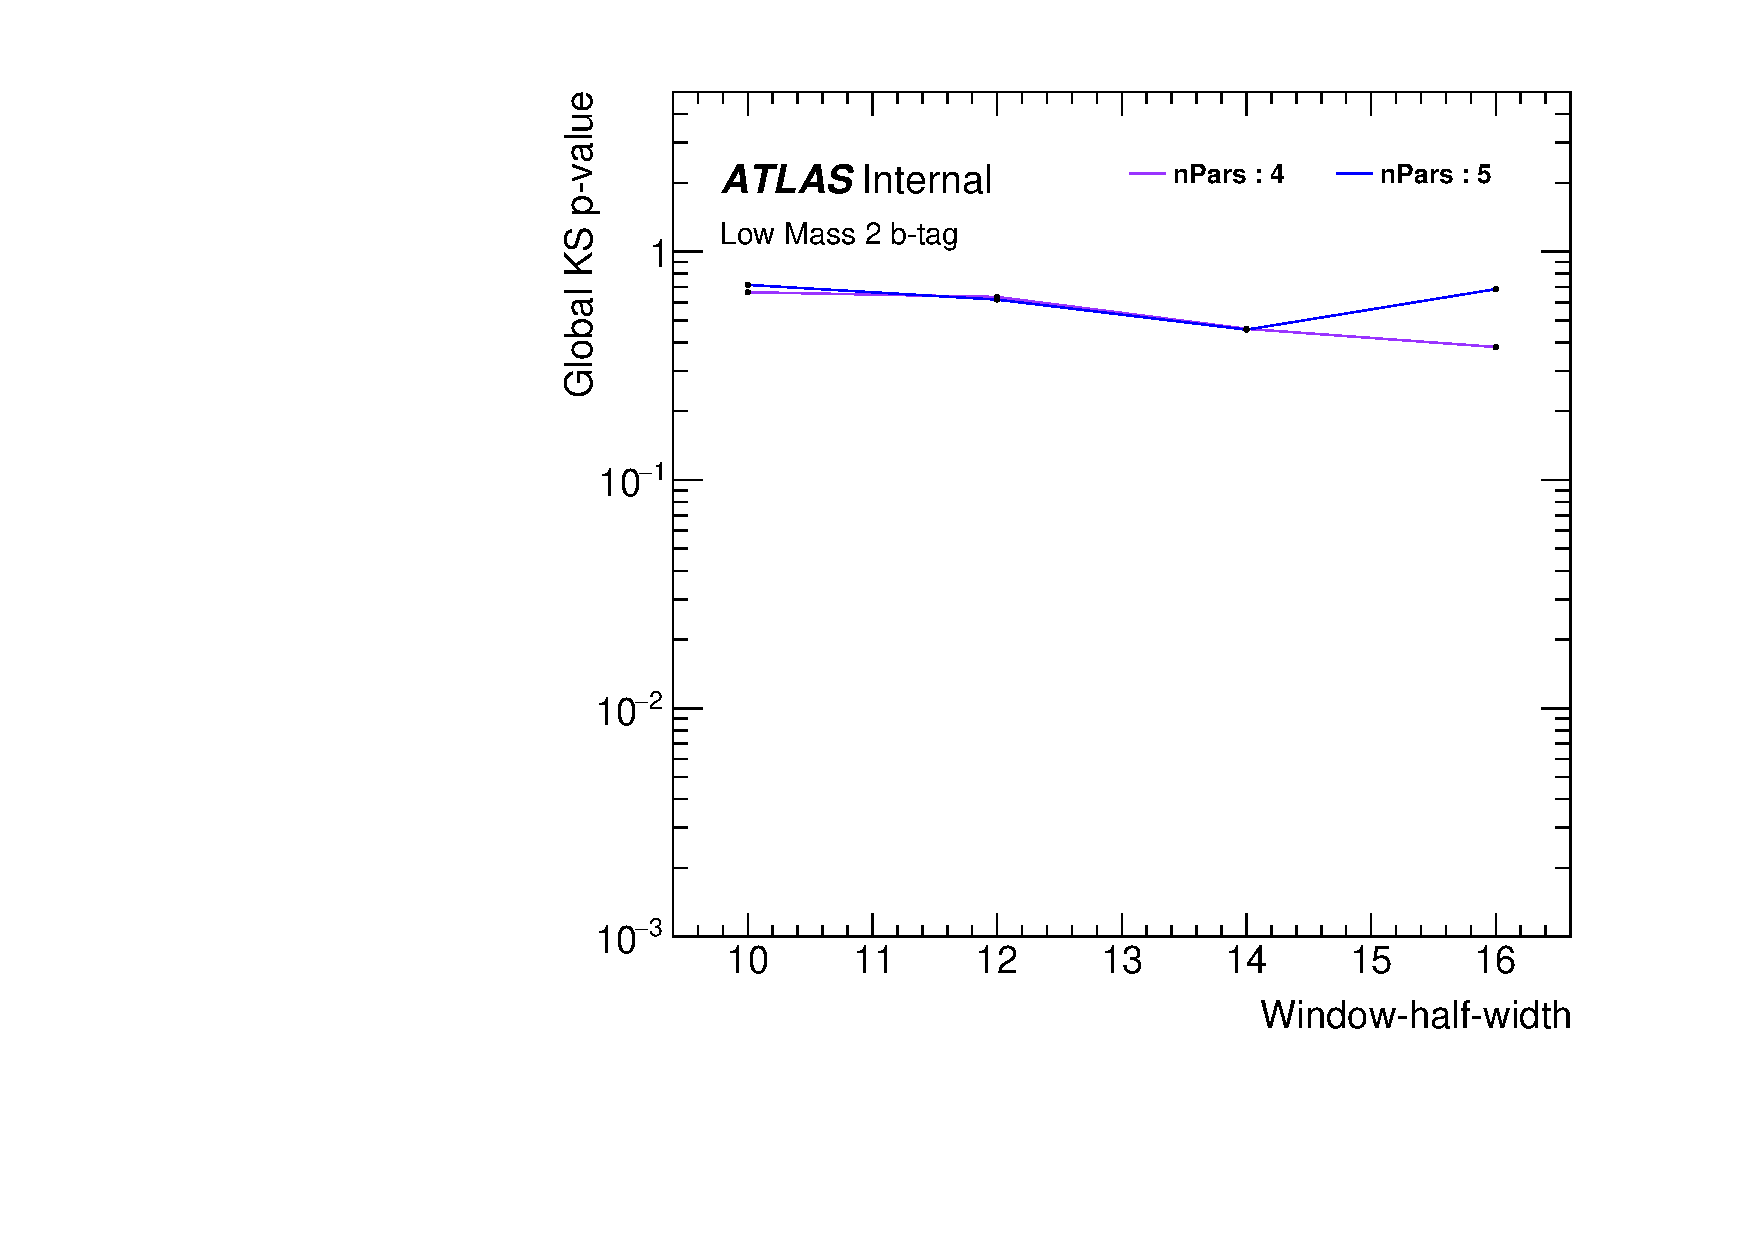
\includegraphics[width=0.49\linewidth, angle=0,page=1]{figs/Dibjet/LowMass/FitStudy_min566/windowSel_subset.pdf}
%} \\
\subcaptionbox{Number of window fits with\\ Wilks' \mbox{$p$-value} $<$ 0.1} {
  \includegraphics[width=0.42\linewidth, angle=0,page=4]{figs/Dibjet/LowMass/FitStudy_min566/windowSel_subset_edited.pdf}
}

\vspace{-0.5em}
\caption
    [The window selection procedure for a 3~\ifb{} subset of \lm{} data.]
    {\label{fig:windowSel_subset}
      An illustration of the window selection procedure for a 3~\ifb{} subset of \lm{} data.
      It shows the global $\chi^{2}$ \mbox{$p$-value}
      and number of window fits with Wilks' \mbox{$p$-value} $<$ 0.1 for the SWiFt background estimate
      using a range of window half-widths ($wHW$) and number of parameters (nPars) of the dijet fit function.
      The dotted lines indicate thresholds that are used in the window selection procedure.
    }
\vspace{-1em}
\end{figure}

%It is notable that the window selection procedure for the subset of data has chosen a wide window and
%could have chosen the lower order function, in contrast to the fit control region case. 
%This shows that either the fit control region often selects narrower windows
%because it is not a perfect representation of the true dijet mass spectra
%or because at the higher precision of the 24.3~\ifb{} narrower windows are required than at 3~\ifb{}.
%Either way, this shows the utility of choosing the window width on the final data-set using a pre-defined procedure.

%\subsubsection{High Mass}
%\label{sec:bkg-full_highmass_windowSelTests} 

\subsection{SWiFt Validation Studies: Spurious Signal}
\label{sec:bkg-full_spuriousSignal}

As described in Section~\ref{sec:bkg-summer_spusig}, it is important to demonstrate that
fit biases and spurious signal will not occur for the SWiFt background estimation strategy,
where a fit bias is a difference between the background estimation
and the true background dijet mass spectrum, and
spurious signal is a false excess caused by a fit bias.

To demonstrate that fit biases are not occurring the SWiFt search phase is performed to background-only representative data-sets
and the \bh{} $p$-values are studied for evidence of spurious signal.
The SWiFt configurations considered use the 4 and 5 parameter dijet fit function
and window half-widths of 10, 12, 14 and 16; giving 8 different configurations.
Only SWiFt configurations that show no evidence of spurious signal are considered in the window selection procedure.

Firstly, we consider the results from the subset of data.
Figure~\ref{fig:bhFit_lm_subset} shows the SWiFt search phase performed on the dijet mass spectrum of the 3~\ifb{} data subset,
for the 4 and 5 parameter dijet fit function for a window half-width of 16.
The blue lines indicate the largest excess found by the \bh{} algorithm and the \mbox{$p$-value} assigned is printed on the plot. 
In both cases the background is well modelled and there is no evidence of spurious signal;
similar results are found for all window half-widths considered.
However, searches for spurious signal using the subset of data are limited by the 
small statistical precision of the subset relative to the final data-set.

\begin{figure}[!htb]
  \vspace{-1.5mm}
\captionsetup[subfigure]{aboveskip=0pt,justification=centering}
\centering
\subcaptionbox{4 parameter function,\\ $wHW$ = 16} {
  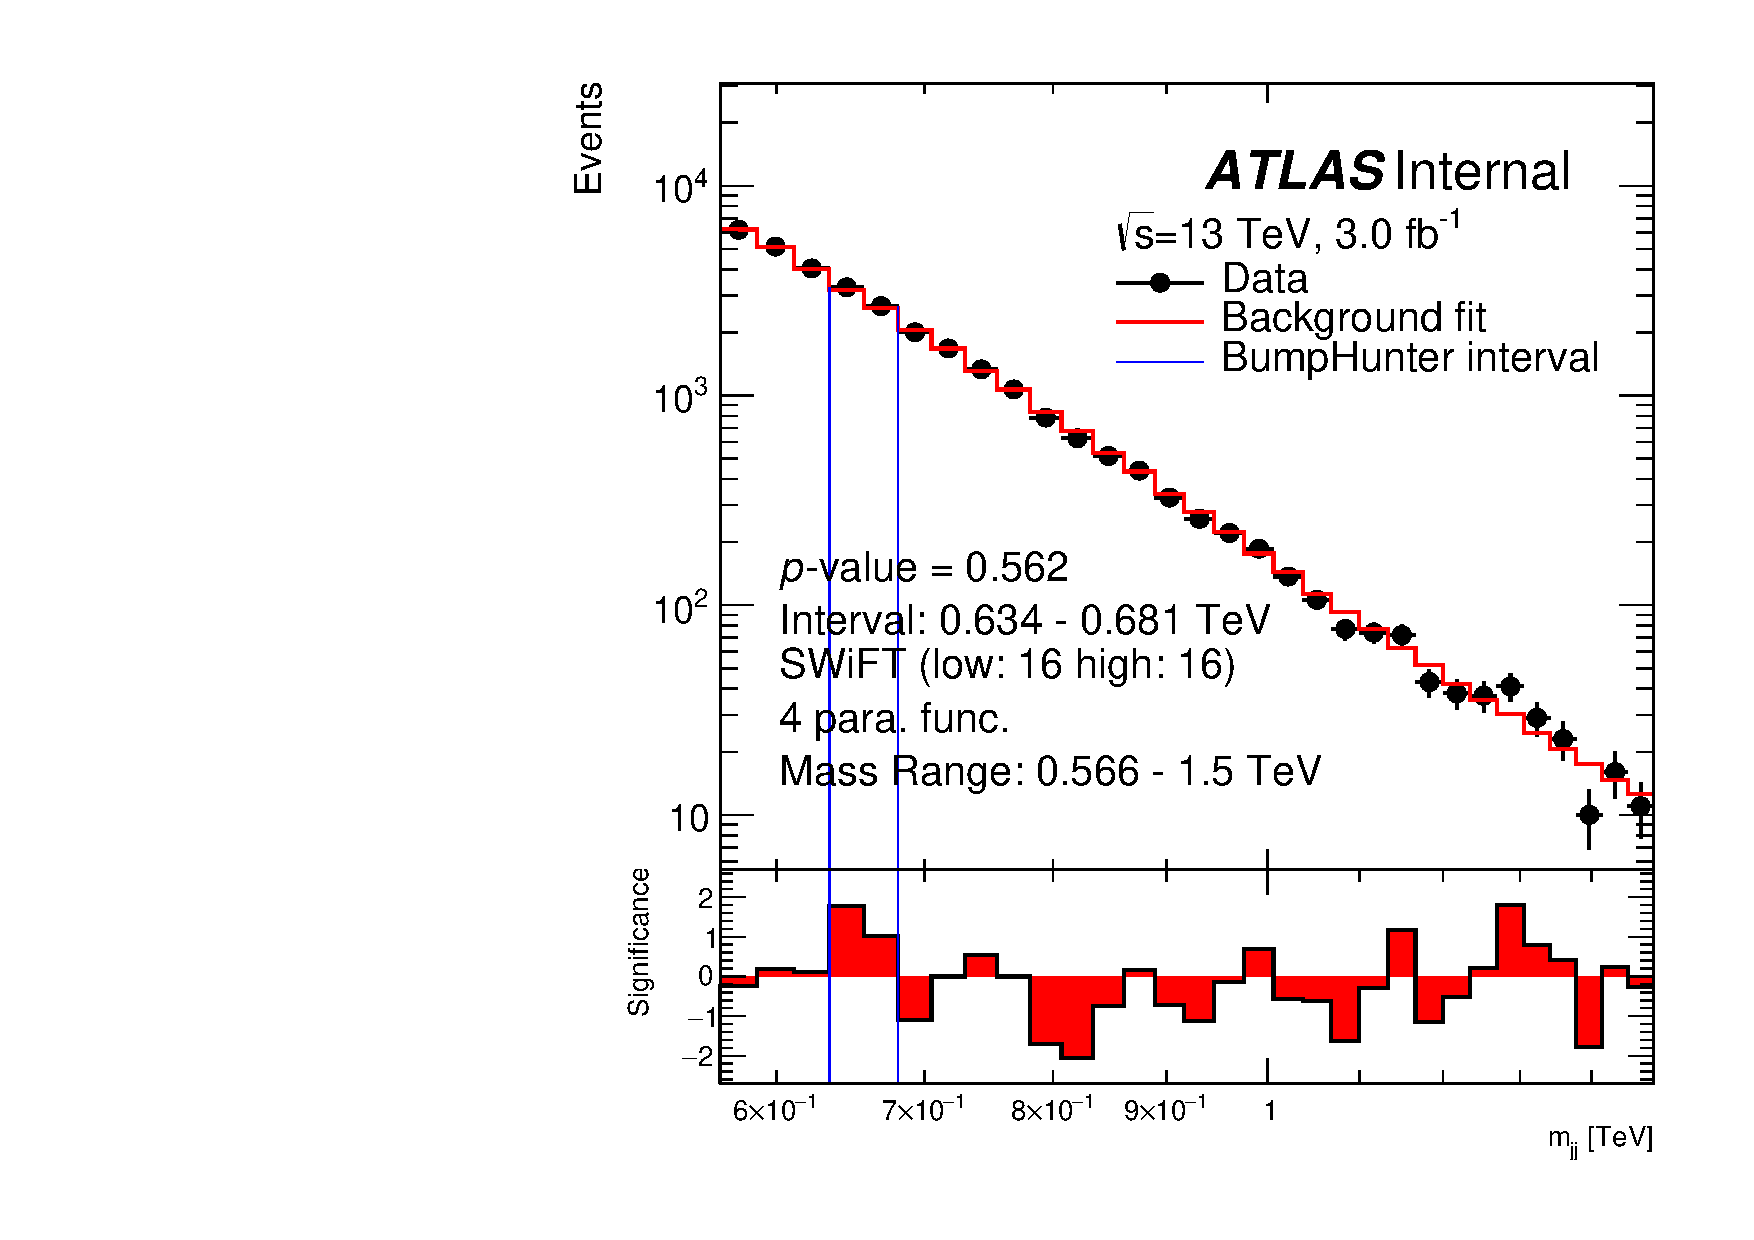
\includegraphics[width=0.42\linewidth, angle=0]{figs/Dibjet/LowMass/FitStudy_min566/bhFit_subset_4para_low16_high16.pdf}
}
\subcaptionbox{5 parameter function,\\ $wHW$ = 16} {
  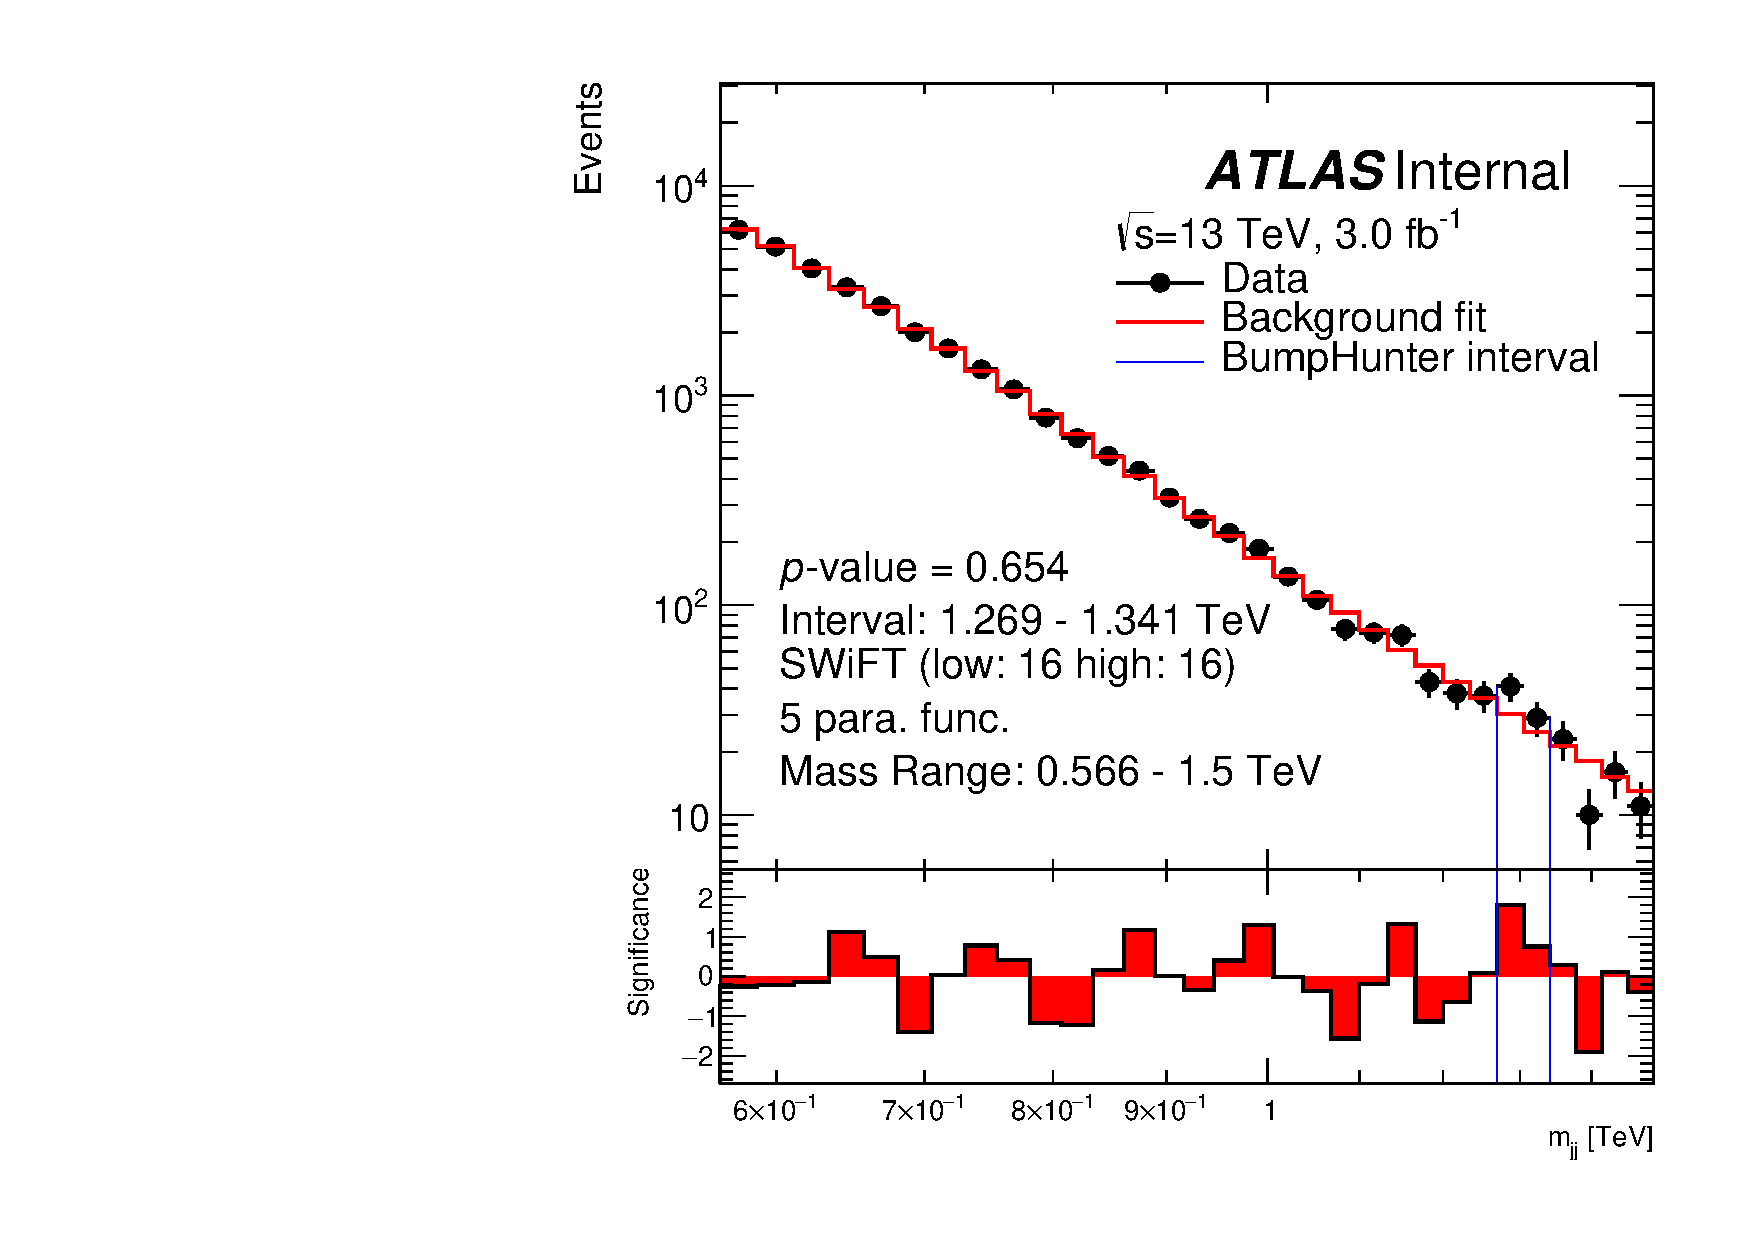
\includegraphics[width=0.42\linewidth, angle=0]{figs/Dibjet/LowMass/FitStudy_min566/bhFit_subset_5para_low16_high16.pdf}
}
%\vspace{-1em}
\caption
    [The SWiFt search phase run on a 3~\ifb{} subset of the \lm{} data-set.]
    {\label{fig:bhFit_lm_subset}
      The SWiFt search phase run on a 3~\ifb{} subset of the \lm{} data-set using the 4 and 5 parameter dijet fit function for a window half-width ($wHW$) of 16.
      The upper panel shows the data compared to the background estimate and the lower panel shows the significance of the difference between the two.
      The most discrepant excess as found by the \bh{} algorithm is indicated by the vertical blue lines and the \mbox{$p$-value} of this excess is printed on the plot. }
\end{figure}

Next, the SWiFt search phase is applied to the smooth dijet mass spectrum from the fit control region
where the uncertainties are set to be Poisson like,
as described in Section~\ref{sec:bkg-full_fitCR}.
Performing the SWiFt search phase to the smooth dijet mass spectra gives a direct comparison
of any fit biases relative to the background fluctuations expected in data.
Figure~\ref{fig:bhFit_lm_corrFitCR_smooth} shows the SWiFt search phase
performed on the smooth dijet mass spectrum taken from the fit control region,
for a SWiFt configuration using the 4 and 5 parameter dijet fit functions and a window half-width of 16 and 10;
the full set of plots for all SWiFt configurations considered are in Appendix~\ref{app:lowMass_Swift}.
%The blue lines indicate the largest excess found by the \bh{} algorithm and the \mbox{$p$-value} assigned is printed on the plot. 

\begin{figure}[!htb]
\captionsetup[subfigure]{aboveskip=0pt,justification=centering}
\centering
\subcaptionbox{4 parameter function,\\ $wHW$ = 16} {
  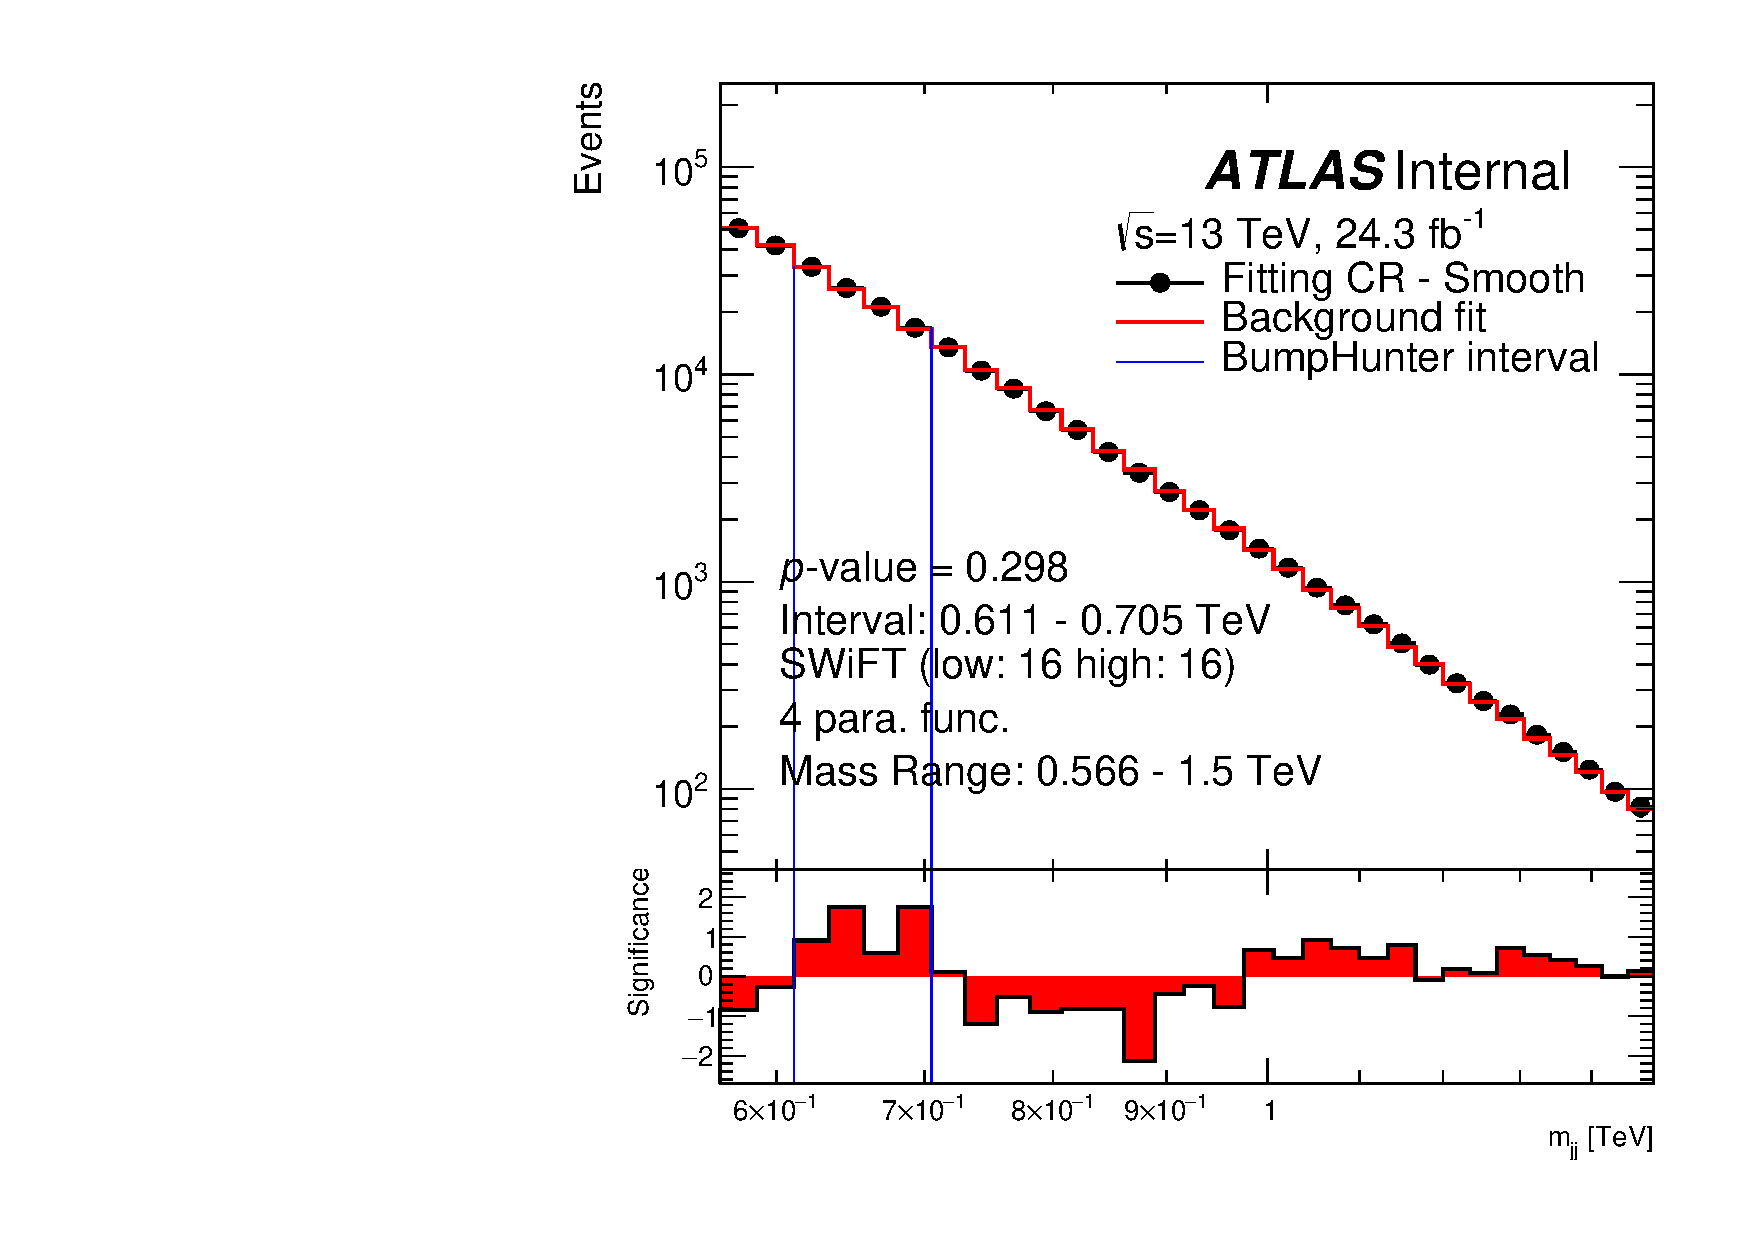
\includegraphics[width=0.42\linewidth, angle=0]{figs/Dibjet/LowMass/FitStudy_min566/bhFit_corrFitCR_smooth_4para_low16_high16.pdf}
}
\subcaptionbox{4 parameter function,\\ $wHW$ = 10} {
  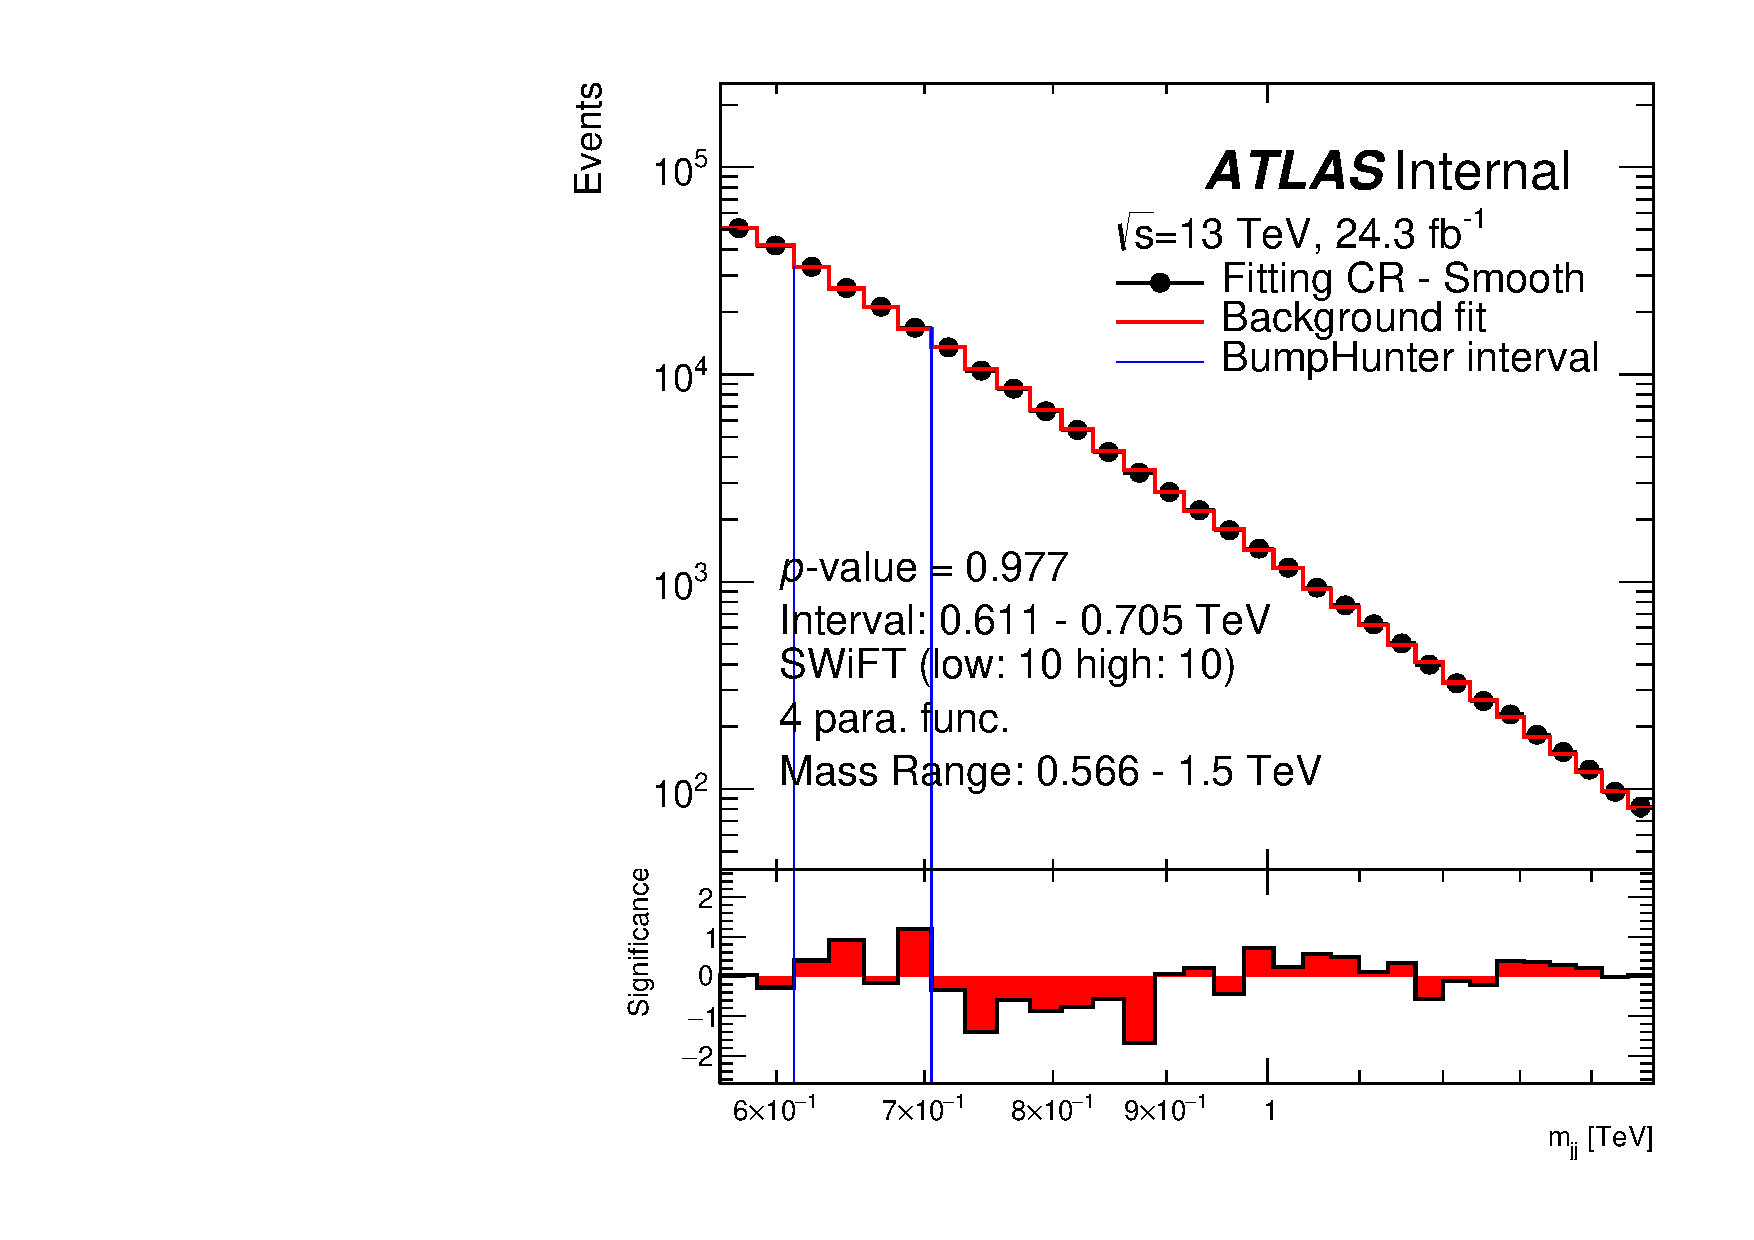
\includegraphics[width=0.42\linewidth, angle=0]{figs/Dibjet/LowMass/FitStudy_min566/bhFit_corrFitCR_smooth_4para_low10_high10.pdf}
}
\subcaptionbox{5 parameter function,\\ $wHW$ = 16} {
  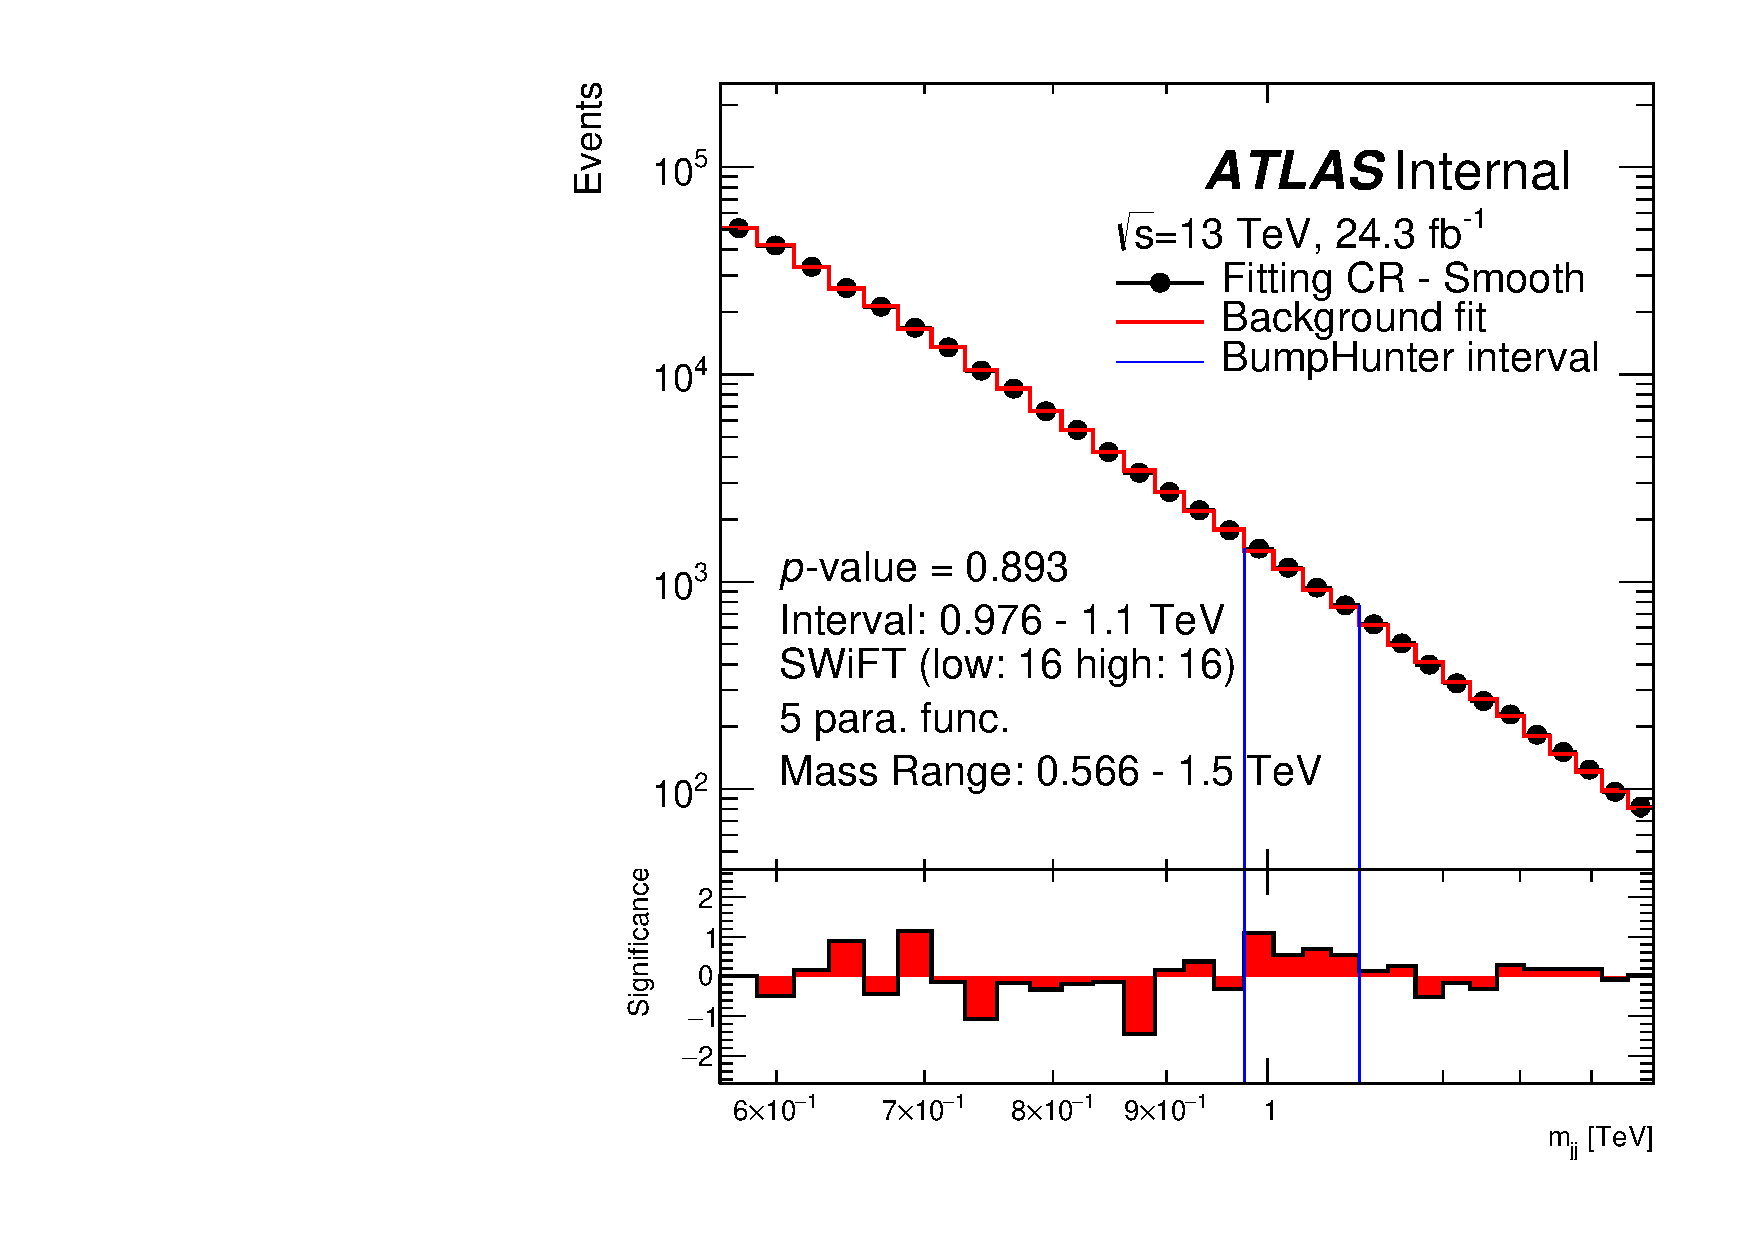
\includegraphics[width=0.42\linewidth, angle=0]{figs/Dibjet/LowMass/FitStudy_min566/bhFit_corrFitCR_smooth_5para_low16_high16.pdf}
}
\subcaptionbox{5 parameter function,\\ $wHW$ = 10} {
  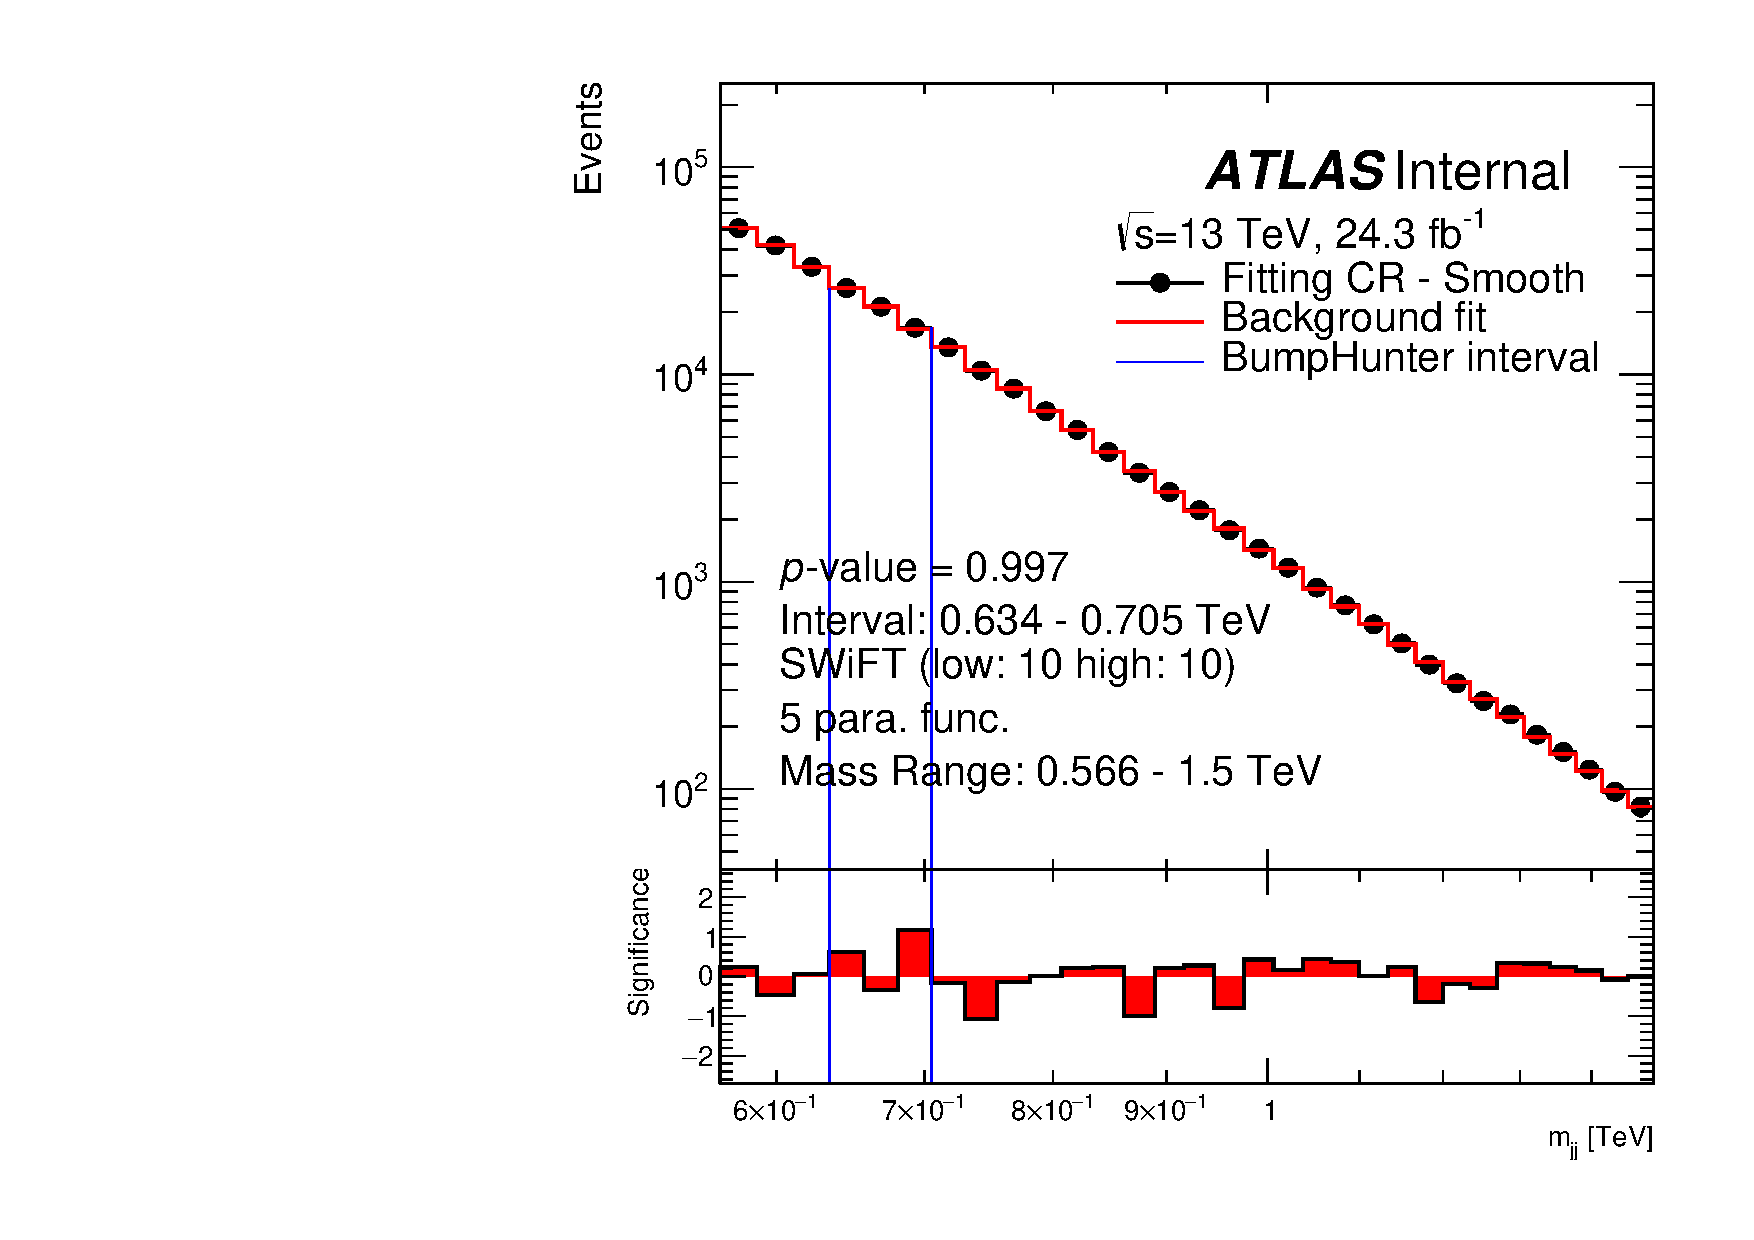
\includegraphics[width=0.42\linewidth, angle=0]{figs/Dibjet/LowMass/FitStudy_min566/bhFit_corrFitCR_smooth_5para_low10_high10.pdf}
}

%\vspace{-1em}
\caption
    [The SWiFt search phase run on the smooth dijet mass spectrum from the \lm{} fit control region.]
    {\label{fig:bhFit_lm_corrFitCR_smooth}
      The SWiFt search phase run on the smooth dijet mass spectrum from the \lm{} fit control region
      using the 4 and 5 parameter dijet fit function for a window half-width ($wHW$) of 10 and 16.
      The upper panel shows the data compared to the background estimate and the lower panel shows the significance of the difference between the two.
      The most discrepant excess as found by the \bh{} algorithm is indicated by the vertical blue lines and the \mbox{$p$-value} of this excess is printed on the plot. }
\end{figure}

As was discussed in Section~\ref{sec:bkg-full_globalFit}, in the case of the smooth spectrum the \bh{} \mbox{$p$-value} provides an approximate estimation
of the size of the largest fit bias relative to the size of the largest excesses expected in data due to statistical fluctuations,
therefore a low $p$-value is an indication that a spurious signal can occur. 
For the 4 parameter dijet fit function with a window half-width of 16 a \bh{} $p$-value of 0.298 is observed indicating that
there is a fit bias which is large relative to the expected statistical fluctuations.
It is also notable that for the 4 parameter dijet fit function there is a large deficit observed in the middle of the mass range for both window half-widths shown.
In the 5 parameter dijet fit function \bh{} $p$-values of 0.826 and 0.987 are observed in the window half-width of 16 and 10 respectively,
which indicates that the largest fit bias is not larger than the size of the excesses expected from statistical fluctuations.

The SWiFt search phase performed on the smooth dijet mass spectrum provides a good visual representation and approximate size of possible fit biases.
However, it is possible that fit biases could enhance statistical fluctuations to create spurious signal in data-sets containing Poisson fluctuations.
To demonstrate that this is not occurring, the SWiFt search phase is applied to many data-like dijet mass spectra,
where Poisson fluctuations are applied to the fit control region as described in Section~\ref{sec:bkg-full_fitCR}.
Figure~\ref{fig:bhFit_lm_corrFitCR_dataLike} shows an example of the SWiFt search phase performed on a data-like dijet mass spectrum taken from the fit control region.
%Again, all 8 window width and fit function choice combinations studied are considered
The SWiFt configurations with a window half-width of 16 for the 4 and 5 parameter dijet fit function are shown, the full set can be found in Appendix~\ref{app:lowMass_Swift}.
%Again, the largest excess found by the \bh{} algorithm and the \mbox{$p$-value} assigned is indicated on the plot.
The fit biases noted in Figure~\ref{fig:bhFit_lm_corrFitCR_smooth} are still visible in the 4 parameter case.
In the 5 parameter case the \bh{} algorithm has not identified a discrepant excess indicating
there is no spurious signal for this particular data-like spectrum.

\begin{figure}[!htb]
\captionsetup[subfigure]{aboveskip=0pt,justification=centering}
\centering
\subcaptionbox{4 parameter function,\\ $wHW$ = 16} {
  \includegraphics[width=0.45\linewidth, angle=0]{figs/Dibjet/LowMass/FitStudy_min566/bhFit_corrFitCR_dataLike_v13_4para_low16_high16.pdf}
}
\subcaptionbox{5 parameter function,\\ $wHW$ = 16} {
  \includegraphics[width=0.45\linewidth, angle=0]{figs/Dibjet/LowMass/FitStudy_min566/bhFit_corrFitCR_dataLike_v13_5para_low16_high16.pdf}
}
\caption
    [The SWiFt search phase run on a data-like dijet mass spectrum of the \lm{} fit control region.]
    {\label{fig:bhFit_lm_corrFitCR_dataLike}
      The SWiFt search phase run on a data-like dijet mass spectrum of the \lm{} fit control region.
      The SWiFt procedure has been run for the 4 and 5 parameter dijet fit function for a window half-width ($wHW$) of 16.
      The upper panel shows the data compared to the background estimate and the lower panel shows the significance of the difference between the two.
      The most discrepant excess as found by the \bh{} algorithm is indicated by the vertical blue lines and the \mbox{$p$-value} of this excess is printed on the plot. 
}
\end{figure}

The SWiFt search phase is performed on 100 data-like dijet mass spectra and the distribution of \bh{} \mbox{$p$-value}s is studied to search for evidence of spurious signal.
500 data-like spectra are used in the case of the 5 parameter fit for window half-widths of 14 and 16
as increased statistical precision is required to make the necessary conclusion for these configurations.
Each data-like spectrum is referred to as a `seed'. %, which denotes the seed used in the random Poisson fluctuation generator.
%In the case of the 5 parameter dijet fit function with a window half-width of 16, which is the widest window that will be used in data and hence the most
%challenging fit that will be performed, this procedure was performed with 450 different data-like distributions to increase statistical precision.

Figure~\ref{fig:bumpH_spuriousSignal} shows the normalised distribution of \mbox{$p$-value}s for the ensemble of data-like dijet mass spectra
for a subset of the SWiFt configurations considered, the full range of plots can be found in Appendix~\ref{app:lowMass_Swift}.
Table~\ref{tab:bumpH_lm_spuriousSignal} shows the percentage of data-like spectra (or seeds)
that have a \bh{} \mbox{$p$-value} less than %0.1,
0.05 and 0.01 for the full range of SWiFt configurations considered;
in particular 0.01 is important as it is the threshold for an excess region to be considered significant enough
to exclude from the background estimation procedure.

For the 4 parameter dijet fit function and a window half-width of 12, 14 and 16
there is a clear bias towards low \bh{} \mbox{$p$-value}s;
in particular significantly more than 1\% of seeds have a \bh{} \mbox{$p$-value} of less than 0.01.
Hence, it is concluded that all SWiFt configurations with the 4 parameter dijet fit function with window half-width greater than 10
show evidence of spurious signal.
For the 4 parameter dijet fit function with a window half-width of 10, there is no evidence of spurious signal;
however this SWiFt configuration is not used as it is less sensitive to signal than SWiFt configurations
using the 5 parameter dijet function with wider windows, as will be shown in Section~\ref{sec:bkg-full_signalInj}.
In the case of all SWiFt configurations using the 5 parameter dijet fit function
there is no significant bias towards low \bh{} \mbox{$p$-value}s,
specifically the number of seeds with a \bh{} \mbox{$p$-value} of less than 0.01 is consistent with expectations.
There is a deficit of seeds with a \bh{} $p$-value $>$ 0.9 for all SWiFt configurations;
this is because the dijet mass spectrum of the fit control region is not perfectly smooth,
as there are small statistical fluctuations present in the 0-tag dijet mass spectrum.

Therefore, it is concluded that for SWiFt configurations using the 5 parameter dijet fit function
there is no evidence that spurious signal can occur in the window half-widths considered.

\begin{table}[!htb]
\centering
\begin{tabular}{|c|c||c|c|c|c|}
  \hline
   \textbf{Dijet Fit}  & \multirow{2}{*}{\textbf{\textit{wHW}}} &\multicolumn{2}{c|}{\textbf{Fraction of Seeds with BH \mbox{$p$-value} \textless}} &   \textbf{Number}   \\ \cline{3-4} 
   \textbf{Function}   &                        & \textbf{0.05}                & \textbf{0.01}                                               &  \textbf{of Seeds}  \\ 
  \hline
  \multirow{4}{*}{4 parameter} &   16 &  31\%   (26-35\%)   &  7.0\% (4-10\%)  & 100  \\
   &   14 &  13\%   (9-16\%)    &  4.0\% (2-6\%)   & 100  \\
   &   12 &  10\%   (7-13\%)    &  4.0\% (2-6\%)   & 100  \\
   &   10 &  2\%   (1-4\%)      &  1.0\% (0-3\%)   & 100  \\
  \hline
  \multirow{4}{*}{5 parameter} &   16 &  4.0\% (3.2-4.9\%)  &  1.2\% (0.8-1.8\%) & 500  \\
  &   14 &  2.4\% (1.8-3.1\%)  &  0.8\% (0.5-1.3\%) & 500  \\
  &   12 &  1\%   (0-3\%)      &  0.0\%  (0-1\%)  & 100  \\
  &   10 &  2\%   (1-4\%)      &  1.0\%  (0-3\%)  & 100  \\
  \hline
\end{tabular}
\caption
    [ The fraction of data-like dijet mass spectra
      with a \bh{} \mbox{$p$-value} less than 0.05 and 0.01,
      for the SWiFt search phase performed on an ensemble of data-like spectra
      taken from the \lm{} fit control region.]
    {\label{tab:bumpH_lm_spuriousSignal}
      The fraction of data-like dijet mass spectra (seeds) 
      with a \bh{} (BH) \mbox{$p$-value} less than 0.05 and 0.01,
      when the SWiFt search phase with the 4 and 5 parameter dijet fit function
      and various window half-widths ($wHW$) is performed on an ensemble of data-like spectra
      taken from the \lm{} fit control region.
      1$\sigma$ confidence interval on the fractions are shown in brackets.
      The number of seeds used for each SWiFt configuration is shown in the table.}
    \vspace{-0.5em}
\end{table}

\begin{figure}[!htb]
\captionsetup[subfigure]{aboveskip=0pt,justification=centering}
\centering
\subcaptionbox{4 parameter function,\\ $wHW$ = 16} {
  \includegraphics[width=0.48\linewidth, angle=0]{figs/Dibjet/LowMass/FitStudy_min566/pVal_bumpHunter_corrFitCR_4para_low16_high16.pdf}
}                                                                                              
\subcaptionbox{4 parameter function,\\ $wHW$ = 10} {                                                    
  \includegraphics[width=0.48\linewidth, angle=0]{figs/Dibjet/LowMass/FitStudy_min566/pVal_bumpHunter_corrFitCR_4para_low10_high10.pdf}
}                                                                                              
\subcaptionbox{5 parameter function,\\ $wHW$ = 16} {                                                    
  \includegraphics[width=0.48\linewidth, angle=0]{figs/Dibjet/LowMass/FitStudy_min566/pVal_bumpHunter_corrFitCR_5para_low16_high16.pdf}
}                                                                                              
\subcaptionbox{5 parameter function,\\ $wHW$ = 14} {                                                    
  \includegraphics[width=0.48\linewidth, angle=0]{figs/Dibjet/LowMass/FitStudy_min566/pVal_bumpHunter_corrFitCR_5para_low14_high14.pdf}
}                                                                                              
\caption[The normalised distributions of \bh{} \mbox{$p$-value}s from performing the SWiFt background estimate on an ensemble of
          data-like dijet mass spectra from the \lm{} fit control region.]
        {\label{fig:bumpH_spuriousSignal}
          The normalised distributions of \bh{} \mbox{$p$-value}s from performing the SWiFt background estimate on an ensemble of
          data-like dijet mass spectra (seeds) from the \lm{} fit control region,
          shown for the 4 and 5 parameter dijet fit function for a selection of window half-widths ($wHW$). 
          The number of data-like spectra used is given on the plot.
}
\vspace{-1em}
\end{figure}

\subsection{SWiFt Validation Studies: Signal Injection}
\label{sec:bkg-full_signalInj}
\vspace{-0.5em}

In the previous two subsections it is shown that the SWiFt background estimate procedure is effective in the case that there is no signal.
However, it is also required to test the SWiFt search phase in the case that signal is present to show that signal can be identified and the remaining background estimate is valid.

To identify signal, the SWiFt search phase uses the \bh{} algorithm to identify the most discrepant excess region and assigns that region a \mbox{$p$-value}.
If the \mbox{$p$-value} is \mbox{$<$ 0.01} then an exclusion region procedure is used to remove any signal induced fit bias in the background estimation.
The exclusion region procedure is as follows.
\vspace{-0.5em}
\begin{enumerate}[leftmargin=*]
\item If a discrepant excess is found, define an exclusion region as the excess region identified by the \bh{} algorithm
      extended on the low mass side by including the dijet mass bin adjacent to the excess region.
      It has been shown that the additional dijet mass bin is required to remove signal induced fit bias~\cite{dijet-mori16_paper}.
      
\item Create an updated background estimate 
      by performing the SWiFt fitting procedure to the dijet mass spectrum, ignoring the exclusion region in all fits and fit quality measures.
\item Identify an updated excess, by performing the \bh{} algorithm to the dijet mass spectrum using the updated background estimate created in Step 3.
      For this step the exclusion region is not ignored.
%\item A new excess is found using the new background estimate and the \bh{} algorithm,
%  the excess can include bins in the exclusion region.
\item If the updated excess is \textit{not} contained within the initial exclusion region,
      then the initial excess region is widened and the procedure returns to Step 2.
      This step ensures that the full effect of the signal induced fit bias is removed.
\item If the updated excess is contained within the initial exclusion region,
      the updated background estimate is tested using the fit quality criteria outlined in Section~\ref{sec:bkg-full_windowSel}.
      If the fit quality criteria is passed, the updated background estimation is used.
      If the fit quality criteria is failed, then a narrower window is tested.
\end{enumerate}
\vspace{-0.25em}
This process will be illustrated with an example below for clarity.

Signal injected dijet mass spectra are used to validate the SWiFt search phase in the case that signal is present.
To create the signal injected spectra, the dijet mass signal templates, described in Section~\ref{sec:evt-s+b},
are added to the data-like dijet mass spectrum taken from the background-only fit control region.
The dijet mass signal templates of a sequential standard model (SSM) $Z'$ boson with generated masses of 600, 800 and 1000 GeV are used in the following studies.
The size of the signal is varied by applying a normalisation factor of 1, 2 or 3 to the simulated signal templates.
Therefore the size of signal in these studies is given relative to the nominal simulated cross-section from {\sc Pythia8};
for example `xs*2' means that a normalisation factor of 2 is used.

\noindent
In the following section two studies with the signal injected spectra are shown:
\vspace{-0.5em}
\begin{enumerate}[leftmargin=*]
  \item\textbf{Sensitivity Studies}\\
  Studies are performed to show that the SWiFt search phase is sensitive to signal,
  and to determine which choices of window half-width and fit function are most sensitive.
  In these studies the SWiFt search phase is applied to the signal injected spectra described above and
  the \bh{} \mbox{$p$-value}s for various SWiFt configurations are studied.
  A \mbox{$p$-value} $<$ 0.01 is considered significant in this study,
  as in these cases the region exclusion procedure would be applied.
  For comparing the sensitivity of two SWiFt configurations a comparison of the
  observed \bh{} \mbox{$p$-value}s is used, where a lower \mbox{$p$-value} indicates a better sensitivity.\vspace{1em}
\item\textbf{Robustness of Window Selection Procedure}\\
    Studies are performed to show that, if signal is present, the window selection procedure is able to select a window and
    the SWiFt search phase can create an adequate description of the background.
    In these studies, the region exclusion and window selection procedure described above is applied
    to SWiFt search phases that find a \bh{} \mbox{$p$-value} $<$ 0.01 in the sensitivity studies.
\end{enumerate}
%\noindent
%Again, the low mass and high mass sections of the analysis are described separately for clarity.

%\subsubsection{Low Mass}
%\label{sec:bkg-full_lowmass_signalInj}
\begin{figure}[!b]
\captionsetup[subfigure]{aboveskip=0pt,justification=centering}
\centering
\subcaptionbox{5 parameter function,\\ $wHW$ = 16} {
  \includegraphics[width=0.45\linewidth, angle=0]{figs/Dibjet/LowMass/FitStudy_min566/bhFit_corrFitCR_dataLike_5para_low16_high16_inj_Zprimebb800_xsFactor1.pdf}
}
\subcaptionbox{5 parameter function,\\ $wHW$ = 14} {
  \includegraphics[width=0.45\linewidth, angle=0]{figs/Dibjet/LowMass/FitStudy_min566/bhFit_corrFitCR_dataLike_5para_low14_high14_inj_Zprimebb800_xsFactor1.pdf}
}\\
\subcaptionbox{5 parameter function,\\ $wHW$ = 12} {
  \includegraphics[width=0.45\linewidth, angle=0]{figs/Dibjet/LowMass/FitStudy_min566/bhFit_corrFitCR_dataLike_5para_low12_high12_inj_Zprimebb800_xsFactor1.pdf}
}
\subcaptionbox{5 parameter function,\\ $wHW$ = 10} {
  \includegraphics[width=0.45\linewidth, angle=0]{figs/Dibjet/LowMass/FitStudy_min566/bhFit_corrFitCR_dataLike_5para_low10_high10_inj_Zprimebb800_xsFactor1.pdf}
}
\vspace{-0.3em}
\caption[The SWiFt search phase run on a data-like dijet mass spectrum
          from the fit control region with a simulated SSM $Z'$ boson of mass 800 GeV injected.]
        {\label{fig:bhFit_lm_corrFitCR_dataLike_inj_Zprimebb800_xsFactor1}
          The SWiFt search phase run on a data-like dijet mass spectrum
          from the fit control region with a simulated SSM $Z'$ boson of mass 800 GeV injected.
          The SWiFt procedure has been run for the 5 parameter dijet fit function for a window half-width ($wHW$) range of 10 to 16.
}
\vspace{-0.7em}
\end{figure}

As an example let's first consider the $Z'$ boson with mass of 800 GeV.
The SWiFt search phase is performed on a data-like dijet mass spectrum
with an injected  $Z'$ boson with mass of 800 GeV and the nominal cross section.
Figure~\ref{fig:bhFit_lm_corrFitCR_dataLike_inj_Zprimebb800_xsFactor1}
shows the results of the SWiFt search phase
using the 5 parameter dijet fit function and a range of window half-widths of 16 to 10.
For all window widths, the \bh{} algorithm has correctly identified the signal region location
and, in the case of the window half-width of 14 and 16, has assigned a significant \mbox{\mbox{$p$-value}} ($<$ 0.01).


Therefore, in the case of the window half-width of 14 and 16 the region exclusion procedure is applied.
The region excluded is 705-834~GeV, derived by adding one bin on the low mass side of the excess region identified by the \bh{} algorithm (730-834~GeV).
Figure~\ref{fig:bhFit_lm_corrFitCR_dataLike_inj_Zprimebb800_xsFactor1_removedWindow} shows the SWiFt search phase
performed on the same spectrum when a region exclusion of 705-834 GeV is applied.
The new excess found lies within the exclusion region which indicates that any signal induced fit bias has been removed
and therefore the exclusion region does not need to be widened.

\begin{figure}[!htb]
\captionsetup[subfigure]{aboveskip=0pt,justification=centering}
\centering
\subcaptionbox{Exclusion Region 705-807 GeV,\\ $wHW$ = 16} {
  \includegraphics[width=0.45\linewidth, angle=0]{figs/Dibjet/LowMass/FitStudy_min566/bhFit_corrFitCR_dataLike_5para_low16_high16_inj_Zprimebb800_xsFactor1_removedWindow.pdf}
}
\subcaptionbox{Exclusion Region 705-834 GeV,\\ $wHW$ = 14} {
  \includegraphics[width=0.45\linewidth, angle=0]{figs/Dibjet/LowMass/FitStudy_min566/bhFit_corrFitCR_dataLike_5para_low14_high14_inj_Zprimebb800_xsFactor1_removedWindow.pdf}
}

%\vspace{-1em}
\caption
    [The SWiFt search phase run on a data-like dijet mass spectrum
      from the fit control region with a simulated SSM $Z'$ boson of mass 800 GeV injected when a region of 705-834 GeV has been excluded from the SWiFt background estimation.]
    {\label{fig:bhFit_lm_corrFitCR_dataLike_inj_Zprimebb800_xsFactor1_removedWindow}
      The SWiFt search phase run on a data-like dijet mass spectrum
      from the fit control region with a simulated SSM $Z'$ boson of mass 800 GeV and the nominal cross-section injected.
      The SWiFt search phase is run for the 5 parameter dijet fit function for a window half-width ($wHW$) of (a) 16 and (b) 14
      with an exclusion region of 705-834~GeV.}
\end{figure}


Figure~\ref{fig:windowSel_Zprimebb800_xsFactor1} shows the fit quality measures used in the window selection procedure after the region exclusion of 705-834 GeV is applied,
for a window half-width of 14 and 16 for the 5 parameter dijet fit function.
Only two window half-widths are considered as these are the only windows that had a significant enough $p$-value to trigger the region exclusion procedure in
Figure~\ref{fig:bhFit_lm_corrFitCR_dataLike_inj_Zprimebb800_xsFactor1}.
The window selection procedure would chose the SWiFt background estimate with the 5 parameter dijet fit function and a window half-width of 14.

Hence, it can be concluded that the SWiFt search phase and region exclusion procedure can identify
a $Z'$ boson with a mass of 800 GeV at the nominal cross-section.
The \bh{} $p$-value assigned after region exclusion is applied is $<$ 0.001 using 10,000 pseudo-experiments;
this shows that the excess has a significance greater than 3~$\sigma$.

\begin{figure}[!htb]
\captionsetup[subfigure]{aboveskip=0pt,justification=centering}
\centering
\subcaptionbox{Global $\chi^{2}$ \mbox{$p$-value}} {
  \includegraphics[width=0.49\linewidth, angle=0,page=6]{figs/Dibjet/LowMass/FitStudy_min566/windowSel_corrFitCR_dataLike_v11_Zprimebb800_xsFactor1_removeWindow.pdf}
}\hspace{-8mm}
\subcaptionbox{Number of window fits with\\ Wilks' \mbox{$p$-value} $<$ 0.1} {
  \includegraphics[width=0.44\linewidth, angle=0,page=8]{figs/Dibjet/LowMass/FitStudy_min566/windowSel_corrFitCR_dataLike_v11_Zprimebb800_xsFactor1_removeWindow_edited.pdf}
}
%\vspace{-1em}
\caption[An illustration of the window selection procedure for a data-like dijet mass spectrum when
          a simulated SSM $Z'$ boson of mass 800 GeV has been injected
          and a region of 705-834 GeV has been excluded from the SWiFt background estimation.]
        {\label{fig:windowSel_Zprimebb800_xsFactor1}
          An illustration of the window selection procedure for a data-like dijet mass spectrum when
          a simulated SSM $Z'$ boson of mass 800 GeV has been injected with the nominal cross-section,
          and a region of 705-834 GeV has been excluded from the SWiFt background estimation.
          The global $\chi^{2}$ \mbox{$p$-value} %global Kolmogorov-Smirnov \mbox{$p$-value}
          and the number of window fits with Wilks' \mbox{$p$-value} $<$ 0.1 of the SWiFt background estimate are shown
          for a range of window half-widths ($wHW$) and the 5 parameter dijet fit function.
          The procedure would have selected the 5 parameter dijet fit function with a window half-width of 14.
}
\end{figure}

\FloatBarrier
Similar tests are performed for a data-like dijet mass spectrum
with a SSM $Z'$ boson injected at masses of 600, 800 and 1000 GeV.
The SWiFt configurations considered use the 4 and 5 parameter dijet fit function and window half-widths ranging from 10 to 16.
The 4 parameter dijet fit function is also considered to compare the sensitivity of the two fit functions.
Table~\ref{tab:bumpH_lm_sigInj} shows the \bh{} \mbox{$p$-value} 
when performing the SWiFt search phase on each of the injected spectra
for all SWiFt configurations considered with no region exclusion applied.
A dash indicates that the largest excess found by the \bh{} algorithm is not consistent with the mass of the injected signal.
Bold text indicates that the SWiFt configuration has a \bh{} $p$-value $<$ 0.01
and is selected by the window selection procedure after the region exclusion procedure has been applied.

\noindent
There are four important conclusions that are taken from Table~\ref{tab:bumpH_lm_sigInj}.

Firstly, all SWiFt configurations are able to obtain a \bh{} $p$-value $<$ 0.01 if the cross-section is high enough.
At 800 GeV the cross-section required is that of the nominal Monte-Carlo simulation, whilst for the 600 and 1000 GeV points
the cross-section needs to be increased to 3 and 2 times respectively.
For the $Z'$ boson at 600 GeV, a large cross-section is required indicating that
there is a signal induced fit bias in this case;
this is due to the fact that the generated mass is close to the low mass edge of the 
dijet mass spectrum, meaning there is no side-band to constrain the background estimate at a dijet mass of 600 GeV.

Secondly, for all signals considered that trigger the region exclusion procedure a window width can be selected;
this shows that the region exclusion and window selection procedure is robust in the case that signal is present.

Thirdly, SWiFt configurations that use large window half-widths are more sensitive;
which can be seen by comparing \bh{} $p$-values for identical injected signals across SWiFt configurations in Table~\ref{tab:bumpH_lm_sigInj}.
Take for example the case when the simulated mass is 800~\GeV{},
the signal normalisation is 1 and the 5 parameter dijet fit function is used;
we see that the $p$-value observed for the widest window considered ($wHW = 16$)
is notably lower than the narrowest window considered ($wHW = 10$),
indicating that the wider window is more sensitive to signal.
This case is particularly notable as only for the two widest widths considered
($wHW =$ 16 or 14) is the $p$-value
below the threshold to trigger the window exclusion procedure.
Furthermore, in all but one of the rows shown in Table~\ref{tab:bumpH_lm_sigInj}
the widest window considered has a $p$-value $<$ 0.01 which would trigger the exclusion region procedure
or has a $p$-value lower than or equal to the $p$-value of the narrowest window considered;
this shows that overall the best sensitivity to signal is found by using a large window-half-width. 

\begin{table}[!hb]
\centering
\begin{tabular}{|c|c|c||c|c|c|c|}
\hline
      Simulated      & Signal             & \multirow{2}{*}{nPars} &\multicolumn{4}{c|}{Window Half-Width} \\ \cline{4-7} 
      Mass [GeV]     & Norm.     &                        &      10        &      12        &      14        &      16        \\ \hline
      \multirow{4}{*}{600}&       \multirow{2}{*}{2}              &           4            &   0.061    &   0.071    &     -      &     -      \\
                     &                           &           5            &   0.110    &   0.093    &   0.104    &   0.045    \\ \cline{2-7}
                     &            \multirow{2}{*}{3}              &           4            &   $<$0.001 &   0.001    &   0.001    &   0.005    \\
                     &                           &           5            &   0.003    &   0.001    &   0.001    &  \textbf{$<$0.001} \\ \hline
      \multirow{4}{*}{800}&       \multirow{2}{*}{1}              &           4            &   0.100    &   0.069    &     -      &     -      \\
                     &                           &           5            &   0.085    &   0.011    &   \textbf{0.007}    &   0.007    \\ \cline{2-7}
                     &            \multirow{2}{*}{2}              &           4            &   $<$0.001 &   $<$0.001 &   $<$0.001 &   $<$0.001  \\
                     &                           &           5            &   \textbf{$<$0.001} &   $<$0.001 &   $<$0.001 &   $<$0.001  \\ \hline
       \multirow{4}{*}{1000}&     \multirow{2}{*}{1}              &           4            &   0.120    &   0.112    &   0.098    &   0.074    \\
                     &                           &           5            &     -      &     -      &   0.107    &   0.093    \\ \cline{2-7}
                     &            \multirow{2}{*}{2}              &           4            &   $<$0.001 &   $<$0.001 &   $<$0.001 &   $<$0.001  \\
                     &                           &           5            &   $<$0.001 &   $<$0.001 &   $<$0.001 &   \textbf{0.001}    \\
\hline
\end{tabular}

%\vspace{-1em}
\caption
    [The  \bh{} \mbox{$p$-value} when performing the SWiFt search phase to
      a data-like dijet mass spectrum that has been injected with a SSM $Z'$ boson with
      a variety of generated masses and normalisation factors.]
    {\label{tab:bumpH_lm_sigInj}
      The  \bh{} \mbox{$p$-value} when performing the SWiFt search phase with no region exclusion applied
      on a data-like dijet mass spectrum that has been injected with a sequential standard model $Z'$ boson with
      a variety of generated masses when the cross-section has been multiplied by a normalisation factor 1, 2 or 3 (Signal Norm.).
      The SWiFt search phase has been performed using a window half-width range of 10 to 16
      and the number of parameters used in the dijet fit function (nPars) are 4 or 5.
      A dash indicates that the largest excess found by \bh{} algorithm is not consistent with the generated mass of the injected signal.
      Bold text indicates that the SWiFt configuration has a \bh{} $p$-value $<$ 0.01
      and is selected by the window selection procedure after the region exclusion procedure has been applied. }
\end{table}

\newpage
The fourth conclusion is that the SWiFt search phase
with a 4 parameter dijet function and window half-width of 10 provides better sensitivity
than the SWiFt search phase with a 5 parameter dijet fit function and a window half-width of 16.
This can be concluded from Table~\ref{tab:bumpH_lm_sigInj} by noting that,
for all signals considered,
the 5 parameter dijet fit function and window half-width of 16
has a $p$-value that can trigger the exclusion region procedure (\mbox{$<$ 0.01})
or has a $p$-value lower than or equal to the $p$-value when using the 4 parameter dijet fit function and window half-width of 10. 
The final two conclusions are important factors in the development of the window selection procedure, described in Section~\ref{sec:bkg-full_windowSel}.

It should also be noted that all \bh{} $p$-values shown in Table~\ref{tab:bumpH_lm_sigInj} are before region exclusion is applied.
The \bh{} \mbox{$p$-value}s are always smaller after region exclusion is applied
as the effect of any signal induced fit bias in the background estimation has been removed;
this has been shown in the case of the $Z'$ boson at a mass of 800 GeV.

To conclude the search phase validation studies for the \lm{} data-set analysis,
it has been shown the SWiFt search phase is
able to provide an adequate background estimation 
and that there is no evidence that spurious signal can occur.
It has also been shown that 
the SWiFt search phase is able to identify a
$Z'$ boson with a generated mass of 600, 800 and 1000 GeV if the cross-section is large enough.

\vspace{0.5em}
\subsection{Results of Window Selection Procedure}
\label{sec:bkg-full_windowSelResults}
%\subsubsection{Low Mass}
%\label{sec:bkg-lowmass_results}

For the full \lm{} data-set a window half-width is chosen using the window selection procedure outlined in Section~\ref{sec:bkg-full_windowSel}.
The SWiFt background estimation is performed using the 5 parameter dijet fit function and a window half-width range of 16 to 10.

For each SWiFt configuration, Figure~\ref{fig:windowSel_unblind} shows the two fit quality measures used in the window selection procedure:
the global $\chi^2$ $p$-value and the number of windows with a Wilks' $p$-value $<$ 0.1.
The requirements placed on each fit quality measure by the window selection procedure are indicated by dotted lines on the figure.
A window half-width of 16 is selected as it is the widest window that passes the fit quality criteria.

\begin{figure}[!htb]
\captionsetup[subfigure]{aboveskip=0pt,justification=centering}
\centering
\subcaptionbox{Global $\chi^{2}$ \mbox{$p$-value}} {
  \includegraphics[width=0.45\linewidth, angle=0,page=6]{figs/Dibjet/LowMass/FitStudy_min566/windowSel_unblind.pdf}
}\hspace{-5mm}
\subcaptionbox{Number of window fits with\\ Wilks' \mbox{$p$-value} $<$ 0.1} {
  \includegraphics[width=0.4\linewidth, angle=0,page=8]{figs/Dibjet/LowMass/FitStudy_min566/windowSel_unblind_edited.pdf}
}
\vspace{2pt}
\caption
    [The window selection procedure for the full \lm{} data-set.]
    {\label{fig:windowSel_unblind}
      An illustration of the window selection procedure for the full \lm{} data-set.
      It shows the global $\chi^{2}$ \mbox{$p$-value} and number of window fits with Wilks' \mbox{$p$-value} $<$ 0.1
      for the SWiFt background estimate using a range of window half-widths and the 5 parameter dijet fit function.
      The dotted lines indicate the requirements used in the window selection procedure. A window half-width of 16 is selected.
    }
\end{figure}

\newpage
Figure~\ref{fig:windowSel_unblind_just16} shows the Wilks' $p$-value and $\chi^2$ $p$-value for fits in each of the windows
as a function of the window centre for the SWiFt background estimation using the 5 parameter dijet fit function and a window half-width of 16,
further showing that all fits used in the SWiFt background estimation are of good quality.

\begin{figure}[!htb]
\captionsetup[subfigure]{aboveskip=0pt,justification=centering}
\centering
\subcaptionbox{$\chi^{2}$ \mbox{$p$-value}} {
  \includegraphics[width=0.43\linewidth, angle=0,page=4]{figs/Dibjet/LowMass/FitStudy_min566/windowSel_unblind_just16.pdf}
}\hspace{-5mm}
\subcaptionbox{Wilks' \mbox{$p$-value}} {
  \includegraphics[width=0.43\linewidth, angle=0,page=1]{figs/Dibjet/LowMass/FitStudy_min566/windowSel_unblind_just16.pdf}
}
\vspace{1pt}
\caption
    [ The  $\chi^{2}$ \mbox{$p$-value} and Wilks' \mbox{$p$-value} for each window fit in the SWiFt background estimate
      performed on the full \lm{} data-set.
    ]
    {\label{fig:windowSel_unblind_just16}
      The  $\chi^{2}$ \mbox{$p$-value} and Wilks' \mbox{$p$-value} for each window fit in the SWiFt background estimate
      performed on the full \lm{} data-set, shown as a function of the window centre.
      The 5 parameter dijet fit function with a window half-width ($wHW$) of 16 is used as the SWiFt configuration.
      The dotted lines indicate thresholds that are used in the window selection procedure.
}
\end{figure}

\FloatBarrier
\clearpage

\subsection{Search Phase Results}
\label{sec:bkg-full_results}

Figure~\ref{fig:bhFit_lm_unblind} shows the dijet mass spectrum of the full \lm{} data-set
and the SWiFt background estimation created using the 5 parameter dijet fit function and a window half-width of 16.
The \bh{} algorithm has identified the most discrepant excess, indicated in the figure using vertical blue lines,
and assigned the excess a \mbox{$p$-value} of 0.603, which has been calculated using 10,000 pseudo-experiments.

The \bh{} $p$-value is 0.603, showing that no significant excess is observed.
Therefore it is concluded that there is no evidence of a BSM resonance in the \lm{} data-set.
As no significant excess is found, the \lm{} data-set is used to set limits on the benchmark signal models,
which will be described in Chapter~\ref{sec:lim}.

\begin{figure}[!thb]
\captionsetup[subfigure]{aboveskip=0pt,justification=centering}
\centering
  \includegraphics[width=0.7\linewidth, angle=0]{figs/Dibjet/LowMass/FitStudy_min566/bhFit_unblind_5para_low16_high16.pdf}
\vspace{3pt}
\caption[The dijet mass spectrum of the \lm{} data-set and the SWiFt background estimation.
        The most discrepant excess found by the \bh{} algorithm and the associated \mbox{$p$-value} are shown.]
        {\label{fig:bhFit_lm_unblind}
   The dijet mass spectrum (\mjj) of the \lm{} data-set and the SWiFt background estimation
   created using the 5 parameter dijet fit function and a window half-width ($wHW$) of 16. 
   The upper panel shows the data compared to the background estimate and the lower panel shows the significance of the difference between the two.
   The most discrepant excess found by the \bh{} algorithm is indicated by the vertical blue lines and the \mbox{$p$-value} of this excess is printed on the plot. }
\end{figure}




%\subsubsection{High Mass}
%\label{sec:bkg-highmass_results}
